\documentclass[a4paper,oneside]{book}
\usepackage{mystyle}
\title{\fontsize{6cm}{1pt}\textbf{GATE 2015}}

\author{
      \fontsize{0.75cm}{1pt}\textbf{Praneeth A S (UG201110023)}\\ 
      \textbf{B.Tech(Computer Science \& Engineering)}\\ \\ \\ \\ 
      \\ \\ \\ \\ \\ \\ \\ \\ \\ \\ \\ \\ \\ \\ \\ \\ 
      \textbf{Indian Institute of Technology Jodhpur}\\
              Jodhpur, Rajasthan 342011,  India    \\
}
\date{\today}

\begin{document}

\maketitle
\pagenumbering{roman} 
\hypertarget{TitlePage}{}
\bookmark[dest=TitlePage,level=-1]{Title Page}
\maketitle
   \hypertarget{Dedication}{}
    \bookmark[dest=Dedication,level=-1]{Dedication}
    \thispagestyle{empty}
    \null\vspace{\stretch {1}}
        
        %\vspace{20cm}
        \begin{center}
        \textbf{Dedicated to my beloved parents who have stood beside me entire my career.}
        \end{center}
        %\vspace{15cm}
\vspace{\stretch{2}}\null
    \hypertarget{Acknowledgements}{}
        \bookmark[dest=Acknowledgements,level=-1]{Acknowledgements}
        \thispagestyle{empty}
    %\null\vspace{\stretch {1}}
        \begin{flushleft}
                \fontsize{5cm}{1em}\textbf{Acknowledgements} 
                
        \end{flushleft}
        \vspace{2.5cm}
                        Many Sources have been used.
\vspace{\stretch{2}}\null
    \hypertarget{Preface}{}
    \bookmark[dest=Preface,level=-1]{Preface}
    \thispagestyle{empty}
    %\null\vspace{\stretch {1}}
        \begin{flushleft}
                \fontsize{5cm}{1em}\textbf{Preface}
        \end{flushleft}
        \vspace{2.5cm}
          To be used for GATE Preparation.
\vspace{\stretch{2}}\null
    
\hypertarget{tocpage}{}
\tableofcontents
\bookmark[dest=tocpage,level=-1]{Contents}\newpage
\hypertarget{loa}{}
\listofalgorithms
\bookmark[dest=loa,level=-1]{List of Algorithms}
\hypertarget{lof}{}
\listoffigures
\bookmark[dest=lof,level=-1]{List of Figures}
\hypertarget{lot}{}
\listoftables
\bookmark[dest=lot,level=-1]{List of Tables}
\hypertarget{lol}{}
\listoflistings
\bookmark[dest=lol,level=-1]{List of Programs}
\hypertarget{todo}{}
\listoftodos
\bookmark[dest=todo,level=-1]{List of Doubts}
\newpage
\pagenumbering{arabic} 
\part{Algorithms}
\label{part:Algorithms}
\chapter{Test}
\begin{algorithm}[H]
\caption{Calculate $y = x^n$}
\label{alg1}
\begin{algorithmic}[1]
\REQUIRE $n \geq 0 \vee x \neq 0$
\ENSURE $y = x^n$
\STATE $y \leftarrow 1$
\IF{$n < 0$}
\STATE $X \leftarrow \frac{1}{x} $
\STATE $N \leftarrow -n$
\ELSE
\STATE $X \leftarrow x$
\STATE $N \leftarrow n$
\ENDIF
\WHILE{$N \neq 0$}
\IF{$N$ is even}
\STATE $X \leftarrow X \times X$
\STATE $N \leftarrow N / 2$
\ELSE[$N$ is odd]
\STATE $y \leftarrow y \times X$
\STATE $N \leftarrow N - 1$
\ENDIF
\ENDWHILE
  \COMMENT{end of while}
\end{algorithmic}
\end{algorithm}
\chapter{Complexity Analysis(Asymptotic Notations)}
\section{\texorpdfstring{$\Theta$}{Theta} Notation}
$\Theta$((g(n)) = f(n): $\exists$ positive\index{positive} constants $c_1$,$ c_2$ and $n_0$ such that 
\begin{align}
                  %$$0 \le c_1*g(n) \le  f(n)  \le c_2*g(n) \hspace{1cm} \forall  n \ge n_0$$
 0 &\le c_1g(n) \le  f(n)  \le  c_2g(n) \hspace{1cm} \forall  n \ge n_0            \label{ca:theta_not}
\end{align}
\section{Big O Notation}
O((g(n)) = f(n): $\exists$ positive constants $c_0$ and $n_0$ such that 
\begin{align}
                  %$$0 \le c_1*g(n) \le  f(n)  \le c_2*g(n) \hspace{1cm} \forall  n \ge n_0$$
 0 &\le  f(n)  \le  c_0g(n) \hspace{1cm} \forall  n \ge n_0            \label{ca:bigo_not}
\end{align}
\section{\texorpdfstring{$\Omega$}{Theta} Notation}
$\Omega$((g(n)) = f(n): $\exists$ positive constants $c_0$ and $n_0$ such that 
\begin{align}
                  %$$0 \le c_1*g(n) \le  f(n)  \le c_2*g(n) \hspace{1cm} \forall  n \ge n_0$$
 0 &\le  c_0g(n) \le  f(n)  \hspace{1cm} \forall  n \ge n_0            \label{ca:omega_not}
\end{align}
\chapter{Solving Recurrences}
\section{Substitution Method}
\begin{definition}[Substitution Method]
We make a guess for the solution and then we use mathematical induction to prove the the guess is correct or incorrect.
For example consider the recurrence $T(n) = 2T\left(\dfrac{n}{2}\right) + n$.
\label{def:substitution_method}
\end{definition}
\subsection{Example}
We guess the solution as $T(n) = O(n \log n)$. Now we use induction to prove our guess.
We need to prove that $T(n) \le cn \log n$. We can assume that it is true for values smaller than n.
\begin{align*}
T(n) &= 2T \left(\dfrac{n}{2}\right) + n \\
         & \le c \left(\dfrac{n}{2}\right) \log \left(\dfrac{n}{2}\right) + n \\
         & =  cn \log n - cn \log 2 + n \\
        & =  cn \log n - cn + n \\
       & \le cn \log n
\label{ex:substitution_method}
\end{align*}
\section{Recurrence Tree Method}
Read it from here \href{http://www.geeksforgeeks.org/analysis-algorithm-set-4-master-method-solving-recurrences/}{Recurrence Tree Method}
\section{Master Method}
\begin{figure}[H]
\caption{Master Theorem}
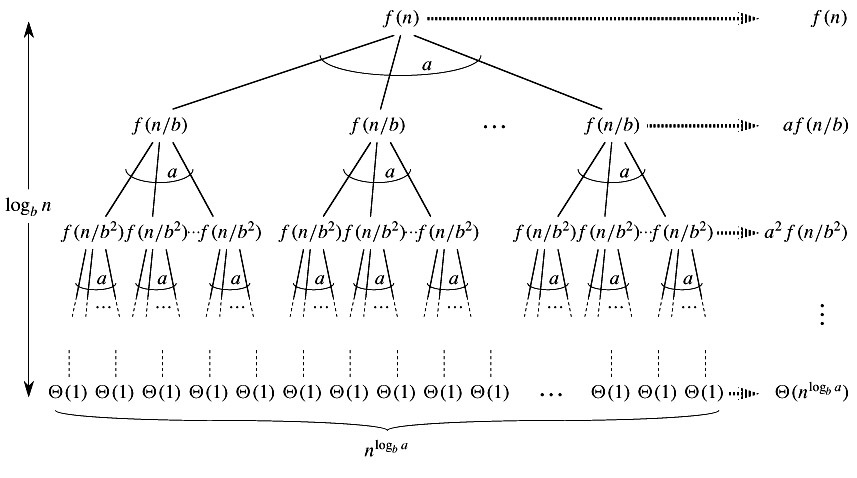
\includegraphics{Images/Master-Theorem}
\label{fig:master_theorem}
\end{figure}
$$ T(n) = aT\left(\dfrac{n}{b}\right) + f(n) $$ where $a \ge 1$ and $ b > 1$ \\
3 cases:
\begin{enumerate}
\item   If f(n) = $\Theta \left(n^{c}\right)$ where $c < \log _{b}a$ then $T(n) = \Theta \left(n^{\log _{b}a}\right)$
\item   If f(n) = $\Theta \left(n^{c}\right)$ where $c = \log _{b}a$ then $T(n) = \Theta \left(n^{c}\log n\right)$
\item   If f(n) = $\Theta \left(n^{c}\right)$ where $c > \log _{b}a$ then $T(n) = \Theta \left(f(n)\right)$
\end{enumerate}
\chapter{Sorting}
\section{Insertion Sort ~\ref{lst:ins_sort}}
\section{Bubble Sort ~\ref{lst:bubble_sort}}
\section{Bucket Sort ~\ref{lst:bucket_sort}}
\section{Heap Sort ~\ref{lst:heap_sort}}
\section{Quick Sort ~\ref{lst:quick_sort}}
\section{Merge Sort ~\ref{lst:merge_sort}}
\section{Summary}
\begin{table}[H]
\begin{tabular}{|l |l |l |l |l |l |l |c |}
\hline
\textbf{Sorting} & \multirow{2}{*}{\textbf{Usage}} & \multicolumn{3}{c|}{\textbf{Time Complexity}} & \textbf{Space} & \textbf{No. of} & \multirow{2}{*}{\textbf{Stability}} \\ \cline{3-5}
\textbf{Method} & & Best & Average & Worst & \textbf{Complexity} & \textbf{swaps} &  \\ \hline
Insertion Sort &&&&&&& \checkmark \\ \hline
Bucket  Sort &&&&&&& \\ \hline
Bubble Sort &&&&&&& \checkmark \\ \hline
Heap Sort &&&&&&& $\times$ \\ \hline
Quick Sort &&&&&&& $\times$ \\ \hline
Merge Sort &&&&&&& \checkmark \\ \hline
\end{tabular}
\caption{Summary of Sorting Methods}
\label{tab:algo_sort}
\end{table}
\textbf{Auxiliary Space} is the extra space or temporary space used by an algorithm. \\
\textbf{Space Complexity} of an algorithm is total space taken by the algorithm with respect to the input size. Space complexity includes both \textbf{Auxiliary space} and \textbf{space used by input.}\\
\textbf{Stability:}  If two objects with equal keys appear in the same order in sorted output as they appear in the input unsorted array. 
\chapter{Searching}
\section{Linear Search}
\section{Binary Search}
\section{Interpolation Search \cite{interpolsearch}}
\marginnote{This is a margin note using the geometry package, set at 0cm vertical offset to the first line it is typeset.}[0cm]
\section{Summary}
\begin{table}[H]
\begin{tabular}{|l |l |}
\hline
\textbf{Method} & \textbf{Time Complexity} \\ \hline
\end{tabular}
\caption{Summary of Search Methods}
\label{tab:algo_search}
\end{table}
\chapter{Divide \& Conquer}
\chapter{Greedy Algorithms}
\section{Introduction}
\textbf{Greedy} is an algorithmic paradigm that builds up a solution piece by piece, always choosing the next piece that offers the most obvious and immediate benefit. Greedy algorithms are used for optimization problems. An optimization problem can be solved using Greedy if the problem has the following property: \textit{At every step, we can make a choice that looks best at the moment, and we get the optimal solution of the complete problem.}\\
\textbf{Examples:} \textit{Kruskal MST, Prim MST, Dijsktra Shortest Path, Huffman Coding, Activity Selection Problem} etc.,
\begin{enumerate}
\item \textbf{Kruskal's Minimum Spanning Tree (MST):} In Kruskal's algorithm, we create a MST by picking edges one by one. The Greedy Choice is to pick the smallest weight edge that doesn't cause a cycle in the MST constructed so far.
\item \textbf{Prim's Minimum Spanning Tree:} In Prim's algorithm also, we create a MST by picking edges one by one. We maintain two sets: set of the vertices already included in MST and the set of the vertices not yet included. The Greedy Choice is to pick the smallest weight edge that connects the two sets.
\item \textbf{Dijkstra's Shortest Path:} The Dijkstra's algorithm is very similar to Prim's algorithm. The shortest path tree is built up, edge by edge. We maintain two sets: set of the vertices already included in the tree and the set of the vertices not yet included. The Greedy Choice is to pick the edge that connects the two sets and is on the smallest weight path from source to the set that contains not yet included vertices.
\item \textbf{Huffman Coding:} Huffman Coding is a loss-less compression technique. It assigns variable length bit codes to different characters. The Greedy Choice is to assign least bit length code to the most frequent character.
\end{enumerate}
\section{Spanning Trees}
\subsubsection{MST}
Given a connected and undirected graph, a spanning tree of that graph is a subgraph that is a tree and connects all the vertices together. A single graph can have many different spanning trees. A \textbf{minimum spanning tree (MST)} or minimum weight spanning tree for a weighted, connected and undirected graph is a spanning tree with weight less than or equal to the weight of every other spanning tree. The weight of a spanning tree is the sum of weights given to each edge of the spanning tree. \\
A minimum spanning tree has ($V - 1$) edges where $V$ is the number of vertices in the given graph.
\subsubsection{Kruskal's MST Algorithm}
\section{Activity Selection Problem}
\begin{definition}[Activity Selection Problem]
You are given n activities with their start and finish times. Select the maximum number of activities that can be performed by a single person, assuming that a person can only work on a single activity at a time.
\end{definition}
\chapter{Dynamic Programming}
\section{Introduction}
\textbf{Dynamic Programming} is an algorithmic paradigm that solves a given complex problem by breaking it into subproblems and stores the results of subproblems to avoid computing the same results again. Following are the two main properties of a problem that suggest that the given problem can be solved using Dynamic programming.\\
\textbf{Example:} Floyd Warshall Algorithm, Bellman Ford Algorithm
\begin{enumerate}
\item \textbf{Overlapping Subproblems:}  Dynamic Programming is mainly used when solutions of same subproblems are needed again and again. In dynamic programming, computed solutions to subproblems are stored in a table so that these don’t have to recomputed. \\
\textbf{Uses:} Fibonacci Numbers
\item \textbf{Optimal Substructure:} A given problems has Optimal Substructure Property if optimal solution of the given problem can be obtained by using optimal solutions of its subproblems.\\
\textbf{For example} the shortest path problem has following optimal substructure property: If a node x lies in the shortest path from a source node u to destination node v then the shortest path from u to v is combination of shortest path from u to x and shortest path from x to v.\\
\textbf{Uses:} Longest Increasing Subsequence, Shortest Path.
\end{enumerate}
Two Approaches:
\begin{enumerate}
\item Memoization (Top Down)
\item Tabulation (Bottom Up)
\end{enumerate}
\section{Fibonacci Numbers}
\section{Ugly Numbers}
\begin{definition}[Ugly Numbers]
\textbf{Ugly numbers} are numbers whose only prime factors are 2, 3 or 5. The sequence $1, 2, 3, 4, 5, 6, 8, 9, 10, 12, 15, \ldots $ shows the first 11 ugly numbers. By convention, 1 is included.
\end{definition}
See ~\ref{lst:dp_ugly} for Dynamic Programming version of problem.
\chapter{NP Classes}
\section{Introduction}
\begin{definition}[P]
 A decision problem that can be solved in polynomial time. That is, given an instance of the problem, the answer yes or no can be decided in polynomial time.
\end{definition}
\begin{definition}[NP]
NP - Non-Deterministic Polynomial Time. A decision problem where instances of the problem for which the answer is yes have proofs that can be verified in polynomial time. This means that if someone gives us an instance of the problem and a certificate (sometimes called a witness) to the answer being yes, we can check that it is correct in polynomial time. \\
A non-deterministically solvable problem by a turing machine(non-deterministic turing machine) in polynomial time.
\end{definition}
\begin{definition}[NP Complete]
A decision problem L is \textbf{NP-complete} if it is in the set of NP problems and also in the set of NP-hard problems. \textbf{NP-complete} is a subset of NP, the set of all decision problems whose solutions can be verified in polynomial time; NP may be equivalently defined as the set of decision problems that can be solved in polynomial time on a non-deterministic Turing machine. A problem p in NP is also NP-complete if every other problem in NP can be transformed into p in polynomial time.\\
A decision problem $C$ is NP-complete if:
\begin{enumerate}
\item $C$ is in NP, and
\item Every problem in NP is reducible to $C$ in polynomial time.
\end{enumerate}
\textbf{Consequence: }If we had a polynomial time algorithm (on a UTM, or any other Turing-equivalent abstract machine) for $C$, we could solve all problems in NP in polynomial time. ie., \textbf{P = NP = NP-Complete}\\
\textbf{Examples:}Boolean satisfiability problem (Sat.), Knapsack problem, Hamiltonian path problem, Travelling salesman problem, Subgraph isomorphism problem, Subset sum problem, Clique problem, Vertex cover problem, Independent set problem, Dominating set problem, Graph coloring problem etc.,
\end{definition}
\begin{definition}[NP Hard]
The precise definition here is that a problem X is \textbf{NP-hard} if there is an NP-complete problem Y such that Y is reducible to X in polynomial time. But since any NP-complete problem can be reduced to any other NP-complete problem in polynomial time, all NP-complete problems can be reduced to any NP-hard problem in polynomial time. Then if there is a solution to one NP-hard problem in polynomial time, there is a solution to all NP problems in polynomial time.\\
If a problem is \textbf{NP-hard}, this means I can reduce any problem in NP to that problem.  This means if I can solve that problem, I can easily solve any problem in NP.  If we could solve an NP-hard problem in polynomial time, this would prove P = NP.\\
\textbf{Examples:} The halting problem is the classic NP-hard problem. This is the problem that given a program P and input I, will it halt? 
\end{definition}
\begin{definition}[Polynomial Reducible]
 Can arbitrary instances of problem Y be solved using a polynomial number of standard computational steps, plus a polynomial number of calls to a black box that solves problem X? \\
Suppose $Y \le_P X$. If X can be solved in polynomial time, then Y can be solved in polynomial time. X is at least as hard as Y (with respect to polynomial time). Y is polynomial-time reducible to X. Suppose $Y \le_P X$. If Y cannot be solved in polynomial time, then X cannot be solved in polynomial time.
\end{definition}
\section{Problem Definitions}
\begin{definition}[Circuit SAT]

\end{definition}
\begin{definition}[]

\end{definition}




\part{Data Structures}
\chapter{Hashing}
\section{Introduction}
\begin{itemize}
\item Prime number to be used for hashing should be very large to avoid collisions.
\item Two keys hash to the same value (this is known as a collision).
\item This hash function involves all characters in the key and can generally be
expected to distribute well (it computes
$\sum_{i=0}^{\text{KeySize-1}}$ Key(KeySize - i - 1) $\times 37^{i}$ and
brings the result into proper range). The code computes a polynomial function (of 37) by use of Horner's rule. For instance, another way
of computing $h_k = k_0 + 37\times k_1 + 37^2 k_2$ is by the formula $h_k =
((k_2)\times7 + k_1 )\times37 + k_0$ .
Horner’s rule extends this to an $n^{th}$ degree polynomial.
\begin{verbatim}
/**
* A hash routine for string objects.
*/
unsigned int hash( const string & key, int tableSize ){
	unsigned int hashVal = 0;
	for( char ch : key )
		hashVal = 37 * hashVal + ch;
	return hashVal % tableSize;
}
\end{verbatim}
\item The first strategy, commonly known as \textbf{separate chaining}, is to keep a list of all elements
that hash to the same value. Might be preferable to avoid their use (since these lists are doubly linked and
waste space)
\item We define the load factor, $\lambda$, of a hash table to be the ratio of the number of elements
in the hash table to the table size. 
\item The average length of a
list is $\lambda$. The effort required to perform a search is the constant time
required to evaluate the hash function plus the time to traverse the list. 
\item In an unsuccessful search, the number of nodes to examine is $\lambda$ on average. 
\item A successful search requires that about 1 + ($\frac{\lambda}{2}$) links be traversed.
\item The general rule
for separate chaining hashing is to make the table size about as large as the number of
elements expected (in other words, let $\lambda \approx$ 1). If the load
factor exceeds 1, we expand the table size by calling \textbf{rehash}.
\item Generally, the load factor should be below $\lambda$ = 0.5 for a hash table that doesn’t use separate chaining. We call such tables \textbf{probing hash tables}.
\item Three common collision resolution strategies:\begin{itemize}
\item Linear Probing
\item Quadratic Probing
\item Double Hashing
\end{itemize}
\item Linear Probing\begin{itemize}
\item In linear probing, f is a linear function of i, typically f(i) = i. This amounts to trying cells
sequentially (with wraparound) in search of an empty cell. Table
~\ref{HashKeyLinearProbing} shows the result of inserting keys {89, 18, 49, 58, 69} into a hash table using the same hash function as before
and the collision resolution strategy, $f(i) = i$.
\item \begin{table}
\centering
\caption{Empty Table}
\label{HashKeyLinearProbing}
\begin{tabular}{|cccccccccc|}
\hline
0 & 1 & 2 & 3 & 4 & 5 & 6 & 7 & 8 & 9\\ \hline
& & & & & & & & & \\ \hline
\end{tabular}
\end{table}
%\begin{table}
\begin{tabular}[H]{|cccccccccc|}
\hline
0 & 1 & 2 & 3 & 4 & 5 & 6 & 7 & 8 & 9\\ \hline
& & & & & & & & & 89\\ \hline
\end{tabular}
%\end{table}
%\begin{table}
\begin{tabular}[H]{|cccccccccc|}
\hline
0 & 1 & 2 & 3 & 4 & 5 & 6 & 7 & 8 & 9\\ \hline
& & & & & & & & 18 & 89\\ \hline
\end{tabular}\\
%\end{table}
%\begin{table}
\begin{tabular}[H]{|cccccccccc|}
\hline
0 & 1 & 2 & 3 & 4 & 5 & 6 & 7 & 8 & 9\\ \hline
49 &  & & & & & & & 18 & 89\\ \hline
\end{tabular}
%\end{table}
%\begin{table}
\begin{tabular}[H]{|cccccccccc|}
\hline
0 & 1 & 2 & 3 & 4 & 5 & 6 & 7 & 8 & 9\\ \hline
 49 & 58 & & & & & & & 18 & 89 \\ \hline
\end{tabular}\\
%\end{table}
%\begin{table}
\begin{tabular}[H]{|cccccccccc|}
\hline
0 & 1 & 2 & 3 & 4 & 5 & 6 & 7 & 8 & 9\\ \hline
49 & 58 & 69 & & & & & & 18 & 89\\ \hline
\end{tabular}\\
%\end{table}
\item Primary clustering, means that any key that hashes into the cluster
will require several attempts to resolve the collision, and then it will add to the cluster.
\end{itemize}
\item Quadratic Probing:\begin{itemize}
  \item $f(i) = i^2$
  \item When 49 collides with 89, the next position attempted is one cell away. This cell is
empty, so 49 is placed there. Next, 58 collides at position 8. Then the cell one
away is tried, but another collision occurs. A vacant cell is found at the next cell tried, which is
$2^2$ = 4 away. 58 is thus placed in cell 2.
\item \begin{table}
\centering
\caption{Empty Table for Quadratic Probing}
\label{HashKeyLinearProbing}
\begin{tabular}{|cccccccccc|}
\hline
0 & 1 & 2 & 3 & 4 & 5 & 6 & 7 & 8 & 9\\ \hline
& & & & & & & & & \\ \hline
\end{tabular}
\end{table}
%\begin{table}
\begin{tabular}[H]{|cccccccccc|}
\hline
0 & 1 & 2 & 3 & 4 & 5 & 6 & 7 & 8 & 9\\ \hline
& & & & & & & & & 89\\ \hline
\end{tabular}
%\end{table}
%\begin{table}
\begin{tabular}[H]{|cccccccccc|}
\hline
0 & 1 & 2 & 3 & 4 & 5 & 6 & 7 & 8 & 9\\ \hline
& & & & & & & & 18 & 89\\ \hline
\end{tabular}\\
%\end{table}
%\begin{table}
\begin{tabular}[H]{|cccccccccc|}
\hline
0 & 1 & 2 & 3 & 4 & 5 & 6 & 7 & 8 & 9\\ \hline
49 &  & & & & & & & 18 & 89\\ \hline
\end{tabular}
%\end{table}
%\begin{table}
\begin{tabular}[H]{|cccccccccc|}
\hline
0 & 1 & 2 & 3 & 4 & 5 & 6 & 7 & 8 & 9\\ \hline
 49 &  & 58 & & & & & & 18 & 89 \\ \hline
\end{tabular}\\
%\end{table}
%\begin{table}
\begin{tabular}[H]{|cccccccccc|}
\hline
0 & 1 & 2 & 3 & 4 & 5 & 6 & 7 & 8 & 9\\ \hline
49 &  & 58 & 69 & & & & & 18 & 89\\ \hline
\end{tabular}\\
\item \begin{theorem}
If quadratic probing is used, and the table size is prime, then a new element can always
be inserted if the table is at least half empty.
\end{theorem}
\end{itemize}
\item Double Hashing\begin{itemize}
  \item For double hash-
ing, one popular choice is f(i) = i.$\text{hash}_2$(x).
\item $\text{hash}_2$(x) must be never evaluated to 0.
\item $\text{hash}_2$(x) = R - (x mod R), with R = 7, a prime smaller than
TableSize
\item The first collision occurs when 49 is inserted. $\text{hash}_2$(49) = 7 -
0 = 7, so 49 is inserted in position 6. $\text{hash}_2$(58) = 7 - 2 = 5, so 58
is inserted at location 3. Finally, 69 collides and is inserted at a distance
$\text{hash}_2$(69) = 7 - 6 = 1 away. If we tried to insert 60 in position 0, we
would have a collision. Since $\text{hash}_2$(60) = 7 - 4 = 3, we would then try
positions 3, 6, 9, and then 2 until an empty spot is found.
\item \begin{table}
\centering
\caption{Empty Table for Double Hashing}
\label{HashKeyLinearProbing}
\begin{tabular}{|cccccccccc|}
\hline
0 & 1 & 2 & 3 & 4 & 5 & 6 & 7 & 8 & 9\\ \hline
& & & & & & & & & \\ \hline
\end{tabular}
\end{table}
%\begin{table}
\begin{tabular}[H]{|cccccccccc|}
\hline
0 & 1 & 2 & 3 & 4 & 5 & 6 & 7 & 8 & 9\\ \hline
& & & & & & & & & 89\\ \hline
\end{tabular}
%\end{table}
%\begin{table}
\begin{tabular}[H]{|cccccccccc|}
\hline
0 & 1 & 2 & 3 & 4 & 5 & 6 & 7 & 8 & 9\\ \hline
& & & & & & & & 18 & 89\\ \hline
\end{tabular}\\
%\end{table}
%\begin{table}
\begin{tabular}[H]{|cccccccccc|}
\hline
0 & 1 & 2 & 3 & 4 & 5 & 6 & 7 & 8 & 9\\ \hline
 &  & & & & & 49 & & 18 & 89\\ \hline
\end{tabular}
%\end{table}
%\begin{table}
\begin{tabular}[H]{|cccccccccc|}
\hline
0 & 1 & 2 & 3 & 4 & 5 & 6 & 7 & 8 & 9\\ \hline
 &  &  & 58 & & & 49 & & 18 & 89 \\ \hline
\end{tabular}\\
%\end{table}
%\begin{table}
\begin{tabular}[H]{|cccccccccc|}
\hline
0 & 1 & 2 & 3 & 4 & 5 & 6 & 7 & 8 & 9\\ \hline
69 &  &  & 58 & & & 49 & & 18 & 89 \\ \hline
\end{tabular}\\
\item If the table size is not prime, it is possible to run out of alternative
locations pre-maturely.
\end{itemize}
\end{itemize}
\section{ReHashing}
\begin{itemize}
  \item As an example, suppose the elements 13, 15, 24, and 6 are inserted into a linear
probing hash table of size 7. The hash function is h(x) = x mod 7.
\begin{tabular}[H]{|ccccccc|}
\hline
0 & 1 & 2 & 3 & 4 & 5 & 6 \\ \hline
6 & 15  &   & 24  &   &   &  13 \\ \hline 
\end{tabular}
\item If 23 is inserted into the table, the resulting table will be over 70 percent
full. Because the table is so full, a new table is created. The size of this table is 17, because
this is the first prime that is twice as large as the old table size. The new hash function is
then h(x) = x mod 17. The old table is scanned, and elements 6, 15, 23, 24, and 13 are
inserted into the new table. The resulting table:\\
\begin{tabular}[H]{|ccccccccccccccccc|}
\hline
0 & 1 & 2 & 3 & 4 & 5 & 6 & 7 & 8 & 9 & 10 & 11 & 12 & 13 & 14 & 15 & 16 \\ \hline 
  &   &   &   &   &   & 6 & 23 & 24 &  &  &  &  & 13 &  & 15 &  \\ \hline
\end{tabular}
\end{itemize}




\part{Theory Of Computation}
References \cite{ullman1979introduction}, Wikipedia articles for definitions of Halting Problem, Recursive Sets etc., \newpage
\chapter{Finite Automaton}
\begin{definition}[DFA,NFA, $\epsilon-NFA$]
\boldmath{$$ M = (Q, \Sigma , \delta, q_0, F) $$}\\
Q : Set of states. In $\epsilon-NFA$ $\epsilon$ is also a state.\\
$\Sigma$ : Set of alphabets\\
$\delta$ : Moving function\\
$q_0$ : Initial State\\
$F$ : Set of Final States. In NFA $2^Q$ is the total no. of possible final states.\\
In $\epsilon-NFA$ $\delta(q_0, 01) = \epsilon-CLOSURE(\delta()\delta(q_0, 0), 1))$.
\end{definition}
\begin{theorem}
If $L$ is accepted by an NFA, there exists an equivalent DFA accepting by $L$.
\end{theorem}
\begin{definition}[$\epsilon$-closure]
$\epsilon$-closure denote the set of all vertices p such that there is a path from q to p labelled $\epsilon$.
\end{definition}
\begin{definition}
If L is accepted by an NFA with $\epsilon$ transitions, then L is accepted by an NFA without $\epsilon$ transitions.
\end{definition}
\begin{definition}
$L^* = \cup_{i=0}^{\infty} L^i$. $L^+ = \cup_{i=1}^{\infty} L^i$
\end{definition}
\begin{theorem}
Let $r$ be a regular expression. Then there exists an NFA with $\epsilon$-transitions that accepts $L(r)$.
\end{theorem}
\begin{definition}[Regular Language]
If $L$ is accepted by DFA, then $L$ is denoted by a regular expression.\\
$R^{k}_{ij} = R^{k-1}_{ik}(R^{k-1}_{ik})^*R_{kj}^{k-1} \cup R_{ij}^{k-1}$\\
$R^{0}_{ij} = \{a| \delta(q_i, a) = q_j \}  if i \neq j$\\
$\{a | \delta(q_i, a) = q_j\} \cup \{\epsilon\}    if i = j$\\
$R^{k}_{ij}$ is the set of all strings that take the finite automaton from state $q_i$ to state $q_j$ without going through any state numbered higher than $k$.
\end{definition}
\chapter{Undecidability}
\section{Definitions}
\begin{definition}[Undecidable Problems]
An \textbf{undecidable problem} is a decision problem for which it is known to be impossible to construct a single algorithm that always leads to a correct yes-or-no answer.
\end{definition}
\begin{definition}[Halting Problem]
Given the description of an arbitrary program and a finite input, decide whether the program finishes running or will run forever. (Undecidable)
\end{definition}
\begin{definition}[Recursive Sets]
A set of natural numbers is called \textbf{recursive}, computable or decidable if there is an algorithm which terminates after a finite amount of time and correctly decides whether or not a given number belongs to the set.
\end{definition}
\begin{definition}[Recursively Enumerable Sets]
A set S of natural numbers is called \textbf{recursively enumerable}, computably enumerable, semidecidable, provable or Turing-recognizable if:
there is an algorithm such that the set of input numbers for which the algorithm halts is exactly S.\\
\textbf{Example:}  Set of languages we can accept using a Turing machine.
\end{definition}
\textbf{NOTE:} There is no algorithm that decides the mebership of a particular string in a language.
\chapter{Turing Machines}
\section{Notation}
\boldmath{$$ M = (Q, \Sigma , \Gamma, \delta, q_0, B, F) $$}
\begin{enumerate}
\item \textbf{Q}: The finite set of states of the finite control.
\item \boldmath{$\Sigma$}: The finite set of input symbols.
\item \boldmath{$\Gamma$}:  The complete set of tape symbols; $\Sigma$ is always a subset of $\Gamma$.
\item \boldmath{$\delta$}: The transition function. The arguments of $\delta(q, X)$ are a state $q$ and a
tape symbol $X$. The value of $\delta(q, X)$, if it is defined, is a triple (p, Y, D ), where:\begin{enumerate}
\item  p is the next state, in Q.
\item Y is the symbol, in $\Gamma$ , written in the cell being scanned, replacing whatever symbol was there.
\item  D is a direction, either Lor R, standing for "left" or "right" respectively, and telling us the direction in which the head moves.
\end{enumerate}
\item {\boldmath$q_0$} : The start state, a member of Q, in which the finite control is found initially.
\item \textbf{B}: The blank symbol. This symbol is in $\Gamma$ but not in E; i.e., it is not an input symbol. T he blank appears initially in all but the finite number of initial cells that hold input symbols.
\item \textbf{F}: The set of final or accepting states, a subset of Q.
\end{enumerate}
 Use the string $X_1X_2\ldots X_{i- 1}qX_iX_{ i+1}\ldots X_n$ to represent an ID in which
\begin{enumerate}
\item  q is the state of the Turing machine.
\item  The tape head is scanning the $i^{th}$ symbol from the left.
\item $X_1X_2\ldots X_n$ the portion of the tape between the leftmost and the rightmost nonblank. As an exception, if the head is to the left of the leftmost nonblank or to the right of the rightmost nonblank, t hen some prefix or suffix of $X_1X_2\ldots X_n$ will be blank, and i will be 1 or n, respectively.
\end{enumerate}
A move M is defined as $X_1X_2\ldots X_{i- 1}qX_iX_{ i+1}\ldots X_n \vdash_M X_1X_2\ldots X_{i-2}pX_{i- 1}X_iX_{ i+1}\ldots X_n$
\begin{figure}[H]
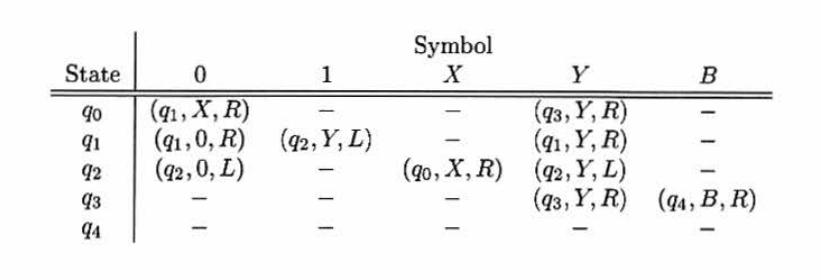
\includegraphics[width=\textwidth,height=\textheight/3]{Images/turingmachine.jpeg}
\caption{Turing machine accepting $0^n1^n \text{ for } n \ge 1$}
\label{fig:turing_machine}
\end{figure}
\unboldmath
\chapter{Regular Sets}
\section{Pumping Lemma}
\textbf{Pumping Lemma} is used to test whether a language is regular or not based on the property that languages obatined from regular languages are regular. If a language is regular,  it is accepted by a DFA $M = (Q, \Sigma, \delta, q_0, F)$ with some particular number of states,  say $n$. 
\begin{lemma}[Pumping Lemma]
 Let $L$ be a regular set. Then there is a constant $n$ such that if $z$ is any word in $L$, and $|z| > n$, we may write $z = uvw$ in such a way that $|uv| \le n, |v| \ge 1$, and for all $i > 0$, $uv^iw$ is in $L$. Furthermore, $n$ is no greater than the number of states of the smallest FA accepting L.
\end{lemma}
\textbf{Examples:}
\begin{enumerate}
\item $0^{i^2} is not a regular language$.
\item  L be the set of strings of 0's and 1's, beginning with a 1, whose value treated as a binary number is a prime. is not a regular language.
 \end{enumerate}
\begin{theorem}
The regular sets are closed under union ($L_1 \cup L_2$), concatenation ($L_1 . L_2$), and Kleene closure ($L^*$).
\end{theorem}
\begin{theorem}
The class of regular sets is closed under complementation. That is, if $L$ is a regular set and $L \in \Sigma^*$,  then $\sigma^* - L$ is a regular set.
\end{theorem}
\begin{theorem}
The regular sets are closed under intersection.
\end{theorem}


\part{Computer Organization \cite{patterson2013computer}}
\chapter{Machine Instructions \& Addressing Modes}
\section{Definitions}
\begin{definition}[Instruction Set] 
\textbf{Instruction set} The vocabulary of commands understood by a given architecture.
\end{definition}
\begin{definition}[Stored Program Concept]
\textbf{Stored-program concept} The idea that instructions and data of many types can be stored in memory as numbers, leading to the stored program computer.
\end{definition}
\begin{definition}[Word]
\textbf{Word} The natural unit of access in a computer, usually a group of 32 bits; corresponds to the size of a register in the MIPS architecture.
\end{definition}
\begin{definition}[Registers]
\textbf{Registers} are limited number of special locations built directly in hardware. The size of a register in the MIPS architecture is 32 bits.
\todo{Is the size of register = word size always? \textbf{Interesting Point}:The word size of an Architecture is often (but not always!) defined by the Size of the General Purpose Registers.}
\end{definition}
\begin{definition}[Data transfer Instructions]
\textbf{Data transfer instruction} A command that moves data between memory and registers. 
\end{definition}
\begin{definition}[Address]
\textbf{Address} A value used to delineate the location of a specific data element within a memory array. To access a word in memory, the instruction must supply the memory \textbf{address}.
\end{definition}
Memory is just a large, single-dimensional array, with the address acting as the index to that array, starting at 0.
\begin{definition}[Base Register]
\end{definition}
\begin{definition}[Offset]
\end{definition}
\begin{definition}[Alignment Restriction]
Words must start at addresses that are multiples of 4(for MIPS). This requirement is called an \textbf{alignment restriction}.
\end{definition}
\begin{definition}[Little \& Big Endian]
Computers divide into those that use the address of the leftmost or \textquotedblleft\textbf{big end}\textquotedblright byte as the word address versus those that use the rightmost or \textquotedblleft\textbf{little end}\textquotedblright byte.
\end{definition}
\begin{definition}[Instruction Format]
\textbf{Instruction format} A form of representation of an instruction composed of fields of binary numbers.
\textbf{Example: } add \$t0, \$s1, \$s2
t0 = 8(reg. no.) s0 = 16(reg.no)\\
\begin{tabular}[H]{|c|c|c|c|c|c|}
\hline
0 & 17 & 18 & 8 & 0 & 32 \\ \hline
000000 & 10001 & 10010 & 01000 & 00000 & 100000 \\ \hline
6 bits & 5 bits & 5 bits & 5 bits & 5 bits & 6 bits \\ \hline
\texttt{op} & \texttt{rs} & \texttt{rt} & \texttt{rd} & \texttt{shamt} & \texttt{funct} \\ \hline 
\end{tabular}
\begin{enumerate}
\item \texttt{op} Basic operation of the instruction, traditionally called the \textbf{opcode}.
\item \texttt{rs} The first register source operand.
\item \texttt{rt} The second register source operand.
\item \texttt{rd} The register destination operand. It gets the result of the operation.
\item \texttt{shamt} Shift amount. (Section 2.5 explains shift instructions and this term;
it will not be used until then, and hence the field contains zero.)
\item \texttt{funct}  Function. This field selects the specific variant of the operation in the
op field and is sometimes called the function code.
\end{enumerate}
\end{definition}
\begin{definition}[Opcode]
An \textbf{opcode} (operation code) is the portion of a machine language instruction that specifies the operation to be performed.
\end{definition}
\begin{definition}[Program Counter]
\textbf{Program counter} (PC) The register containing the address of the instruction in the program being executed.
\end{definition}
\begin{definition}[Addressing Modes]
\textbf{Addressing mode} One of several addressing regimes delimited by their varied use of operands and/or addresses.
\end{definition}
\section{Design Principles}
\begin{enumerate}
\item  \textbf{Simplicity favors regularity}.
\item \textbf{Samller is faster}  A very large number of registers may increase the clock cycle time simply because it takes electronic signals longer when they must travel farther.
\item \textbf{Make common case fast} Constant operands occur frequently, and by including constants inside arithmetic
instructions, they are much faster than if constants were loaded from memory.
\item \textbf{Good design demands good compromises}. Different kinds of instruction formats for different kinds of instructions.
\end{enumerate}
\section{Machine Instructions \cite[p.67,90]{patterson2013computer}}
\begin{enumerate}
\item \textbf{Load} \texttt{lw}: copies data from memory to a register. \textbf{Format:} \texttt{lw} register, mem loc. of data(num,reg. where base add. is stored) 
item \textbf{Store} \texttt{sw}: copies data from register to memory. \textbf{Format:} \texttt{sw} register, mem loc. of data(num,reg. where base add. is stored) 
\item \textbf{Add} \texttt{add}:
\item \textbf{Add Immediate} \texttt{addi}:
\item \textbf{Subtract} \texttt{sub}:
\end{enumerate}
\begin{verbatim}
lw $t0,8($s3) # Temporary reg $t0 gets A[8]
\end{verbatim}
\chapter{Pipelining}
\begin{definition}[Pipelining]
\textbf{Pipelining} is an implementation technique in which multiple instructions are overlapped in execution.
\end{definition}
Pipelining doesn't decrease the time to finish a work but increases the throughput in a given time.
MIPS instrructions takes 5 steps:
\begin{enumerate}
\item Fetch instruction from memory.
\item Read registers while decoding the instruction. The format of MIPS instructions allows reading and decoding to occur simultaneously.
\item  Execute the operation or calculate an address.
\item Access an operand in data memory.
\item Write the result into a register.
\end{enumerate}
$$ \text{Time between instructions}_{\text{pipelined}} = \dfrac{\text{Time between instructions}_{\text{nonpipelined}}}{\text{Number of pipe stages}}$$
Speedup due to pipelining $\approx$ No. of pipe stages. $5$ stage piplelined process is $5$ times faster. (Only for perfectly balanced processes).\\
But process involve overhead. So speedup will be quite less.
\section{Designing Instruction sets for pipelining}
\begin{enumerate}
\item All MIPS instructions are the same length. This restriction makes it much easier to fetch instructions in the first pipeline stage and to decode them in the second stage.
\item MIPS has only a few instruction formats, with the source register fields being located in the same place in each instruction. This symmetry means that the second stage can begin reading the register file at the same time that the hardware is determining what type of instruction was fetched. 
\item Memory operands only appear in loads or stores in MIPS. This restriction means we can use the execute stage to calculate the memory address and then access memory in the following stage.
\item Operands must be aligned in memory. Hence, we need not worry about a single data transfer instruction requiring two data memory accesses; the requested data can be transferred between processor and memory in a single pipeline stage.
\end{enumerate}
\section{Pipeline Hazards}
\subsection{Structural Hazards}
 It means that the hardware cannot support the combination of instructions that we want to execute in the same clock cycle. 
\subsection{Data Hazards}
\textbf{Data hazards} occur when the pipeline must be stalled because one step must wait for another to complete.
\textbf{For example}, suppose we have an add instruction followed immediately by a subtract instruction that uses the sum (\$s0):
\begin{verbatim}
add \$s0, \$t0, \$t1
sub \$t2, \$s0, \$t3
\end{verbatim}
Without intervention, a data hazard could severely stall the pipeline. 
\subsubsection{Solution}
\textbf{Forwarding} also called bypassing. A method of resolving a data hazard by retrieving the missing data element from internal buffers rather than waiting for it to arrive from programmer-visible registers or memory. \\
\textbf{Load-use data hazard} A specific form of data hazard in which the data requested by a load instruction has not yet become available when it is requested. \textbf{Pipeline stall} Also called bubble. A stall initiated in order to resolve a hazard.\\
For \textbf{example} If first instruction were \texttt{load} instead of \texttt{add} then \$s0 would not be available until $4^{\text{th}}$ stage resulting in a pipeline stall.
\subsection{Hazards}
\chapter{Arithmetic for Computers}
\section{Definitions}
\begin{definition}[LSB \& MSB]
\textbf{LSB :} right-most bit .\textbf{MSB :} left-most bit.
\end{definition}
\chapter{Speedup}
\begin{definition}[Amdahl's Law]
content...
\end{definition}
\newpage























\part{First Order Logic}
\chapter{Propositional Logic}
\section{Introduction}
\begin{itemize}
  \item Simple Statement: A simple statement is one that does not contain any
  other statement as a component.\\Ex., Fast foods tend to be unhealthy.
  \item Compound Statement: A compound statement is one that contains at least one simple statement as a
component.\\Ex., Dianne Reeves sings jazz, and Christina Aguilera sings pop.
  \item \begin{tabular}[H]{cccc}
  Operator & Name & Logical function & Used to translate \\ \hline
$\sim$ & tilde & negation & not, it is not the case that \\
$\wedge$ & dot & conjunction & and, also, moreover \\
$\lor$ & wedge & disjunction & or, unless \\
$\to$ & horseshoe & implication & if $\ldots$ then $\ldots$ , only if \\
$\leftrightarrow$ & triple bar & equivalence & if and only if\\
  \end{tabular}
  \item \footnote{S - First Part, P -
  Second
  Part}\begin{tabular}[H]{|>{\centering\arraybackslash}p{1.5cm}p{4.5cm}p{10cm}|}
  \hline
  Symbol & Words & Usage \\ \hline
  \multirow{3}{*}{$\sim$} & doesnot & Rolex does not make computers.\\
  & not the case & It is not the case that Rolex makes computers. \\
  & false that & It is false that Rolex makes computers.\\ \hline
  \multirow{4}{*}{$\wedge$} & \multirow{2}{*}{and} & Tiff any sells jewelry, and Gucci sells cologne. \\
  & & Tiff any and Ben Bridge sell jewelry.\\
  & but & Tiff any sells jewelry, but Gucci sells cologne. \\
  & however & Tiff any sells jewelry; however, Gucci sells cologne. \\ \hline
  \multirow{6}{*}{$\to$} & if $\ldots$,then $\ldots$ (S $\to$ P) & If Purdue
  raises tuition, then so does Notre Dame.\\
  & $\ldots$ if $\ldots$ (P $\to$ S) & Notre Dame raises tuition if Purdue
  does.\\
  & $\ldots$ only if $\ldots$ (S $\to$ P) & Purdue raises tuition only if Notre
  Dame does.\\
  & $\ldots$ provided that $\ldots$ (P $\to$ S) & Cornell cuts enrollment
  provided that Brown does.\\
   & $\ldots$ provided that $\ldots$ (P $\to$ S) & Cornell cuts enrollment on
   condition that Brown does.\\
   & $\ldots$ provided that $\ldots$ (S $\to$ P) & Brown’s cutting enrollment
   implies that Cornell does.\\ \hline
  \multirow{4}{*}{$\lor$} & \multirow{2}{*}{Either $\ldots$ or} & Aspen allows
  snowboards or Telluride does.\\
  & & Either Aspen allows snowboards or Telluride does.\\
  & \multirow{2}{*}{Unless} & Aspen allows snowboards unless Telluride does.\\
  & & Unless Aspen allows snowboards, Telluride does.\\ \hline
  \multirow{2}{*}{$\leftrightarrow$} & $\ldots$ if and only if $\ldots$ (S
  $\to$ P) & JFK tightens security if and only if O’Hare does.\\
   & $\ldots$ sufficient and necessary condition that $\ldots$ (S $\to$ P) & JFK’s tightening security is a suffi cient and
necessary condition for O’Hare’s doing so.\\   \hline
  \end{tabular}
  \item The $\to$ symbol is also used to translate statements phrased in terms
  of sufficient conditions and necessary conditions. Event A is said to be a sufficient condition
for event B whenever the occurrence of A is all that is required for the occurrence of B.
On the other hand, event A is said to be a necessary condition for event B whenever
B cannot occur without the occurrence of A. For example, having the flu is a sufficient
condition for feeling miserable, whereas having air to breathe is a necessary condition
for survival. Other things besides having the flu might cause a person to feel miserable,
but that by itself is suffi cient; other things besides having air to breathe are required for
survival, but without air survival is impossible. In other words, air is
necessary.
\item To translate statements involving sufficient and necessary conditions into symbolic
form, place the statement that names the sufficient condition in the antecedent
of the conditional and the statement that names the necessary condition in the
consequent.
\begin{enumerate}
  \item Hilton’s opening a new hotel is a sufficient
condition for Marriott’s doing so. H $\to$ M
  \item Hilton’s opening a new hotel is a necessary condition
for Marriott’s doing so. M $\to$ H
\end{enumerate}
\item \begin{tabular}[H]{ll}
\hline
Not either A or B. & $\sim$(A $\lor$ B)\\
Either not A or not B. & $\sim$A $\lor$ $\sim$B\\
Not both A and B. & $\sim$(A $\wedge$ B)\\ 
Both not A and not B. & $\sim$A $\wedge$ $\sim$B\\ \hline
\end{tabular}
\end{itemize}
\section{Truth Table}
\begin{multicols}{2}
\begin{itemize}
  \item NEGATION \begin{tabular}[H]{c|c}
p & $\sim$p \\ \hline
0 & 1 \\
1 & 0 \\ 
\end{tabular}
\item AND \begin{tabular}[H]{c|c|c}
p & q & p$\wedge$q \\ \hline
0 & 0 & 0 \\
0 & 1 & 0 \\
1 & 0 & 0 \\
1 & 1 & 1 \\
\end{tabular}
\item OR \begin{tabular}[H]{c|c|c}
p & q & p$\lor$q \\ \hline
0 & 0 & 0 \\
0 & 1 & 1 \\
1 & 0 & 1 \\
1 & 1 & 1 \\
\end{tabular}
\item IF \begin{tabular}[H]{c|c|c}
p & q & p$\to$q \\ \hline
0 & 0 & 1 \\
0 & 1 & 1 \\
1 & 0 & 0 \\
1 & 1 & 1 \\
\end{tabular}
\item IF AND ONLY IF \begin{tabular}[H]{c|c|c}
p & q & p$\leftrightarrow$q \\ \hline
0 & 0 & 1 \\
0 & 1 & 0 \\
1 & 0 & 0 \\
1 & 1 & 1 \\
\end{tabular}
\item To find truth value of long propositions \setlength{\tabcolsep}{1pt}
\begin{tabular}[H]{ccccccccccc}
(&B&$\wedge$&C&)&$\to$&(&E&$\to$&A&)\\
(&T&$\wedge$&T&)&$\to$&(&F&$\to$&T&)\\
\multicolumn{5}{c}{T} & $\to$ & \multicolumn{5}{c}{T} \\ 
\multicolumn{11}{c}{\circled{T}}\\
\end{tabular}
\item \begin{tabular}[H]{|p{3cm}|p{3cm}|}
\hline
Column under main operator & Statement classification \\ \hline
all true tautologous & (logically true)\\ \hline
all false & self-contradictory (logically false)\\ \hline
at least one true, at least one false & contingent\\ \hline
\end{tabular}
\item If all Premises are true and conclusion is false, then argument is
invalid.
\item Assume argument invalid (true premises, false conclusion)\begin{enumerate}
  \item Contradiction $\rightarrow$ Argument is valid
  \item No Contradiction $\rightarrow$ Argument is as assumed (i.e., invalid)
\end{enumerate}
\item Assume statements consistent (assume all of them true) \begin{enumerate}
  \item Contradiction $\rightarrow$ Statements is consistent
  \item No Contradiction $\rightarrow$ Statements is as assumed (i.e.,
  inconsistent)
\end{enumerate}
\end{itemize}
\end{multicols}
\section{Rules}
\begin{tabular}[H]{|l|c|c|c|}
\hline
\multicolumn{4}{|c|}{Rules of Implication}\\
\hline Name & Premises1 & Premises2 & Conclusion \\ \hline
Modus Ponens(MP) & p $\to$ q & p & q\\
Modus Tollens(MT) & p $\to$ q & $\sim$q & $\sim$p \\
Hypothetical Syllogism(HS) & p $\to$ q & q $\to$ r & p $\to$ r \\
Disjunctive Syllogism(DS) & p $\lor$ q & $\sim$p & q\\
Constructive Dilemma(CD) & (p $\to$ q) $\wedge$ (r $\to$ s) & p $\lor$ r & q
$\lor$ s\\
Destructive Dilemma(DD) & (p $\to$ q) $\wedge$ (r $\to$ s) & $\sim q$ $\lor$ $\sim s$ & $\sim p$
$\lor$ $\sim r$\\ 
Conjunction & p & q & p $\wedge$ q\\
Addition & p & & p $\lor$ q\\
Simplification & p $\wedge$ q & & p\\ \hline
\end{tabular}
\\
\begin{tabular}[H]{|l|c|c|}
\hline
\multicolumn{3}{|c|}{Rules of Replacement}\\ \hline
\multirow{2}{*}{De-Morgan's Rule} & $\sim$(p $\wedge$ q) & ($\sim$p $\lor
\sim$q)\\
& $\sim$(p $\lor$ q) & ($\sim$p $\wedge$ $\sim$q) \\ \hline
\multirow{2}{*}{Commutative} & (p $\lor$ q) & (q $\lor$ p) \\
& (p $\wedge$ q) & (q $\wedge$ p) \\ \hline
\multirow{2}{*}{Associative} & p $\lor$ (q $\lor$ r) & (p
$\lor$ q) $\lor$ r \\ 
& p $\wedge$ (q $\wedge$ r) & (p $\wedge$ q) $\wedge$ r \\ \hline
\multirow{2}{*}{Distributive} & p $\wedge$ (q $\lor$ r) &
(p $\wedge$ q) $\lor$ (p $\wedge$ r) \\
& p $\lor$ (q $\wedge$ r) & (p $\lor$ q) $\wedge$ (p $\lor$
r)\\ \hline
Double-Negation & p & $\sim \sim$p\\ \hline
Transposition & p $\to$ q & $\sim q \to \sim p$\\ \hline
Exportation & (p $\wedge$ q) $\to$ r & p $\to$ (q $\to$ r) \\ \hline
Material Implication & p $\to$ q & $\sim$ p $\wedge$ q \\ \hline
 \multirow{2}{*}{Tautology} & \multirow{2}{*}{p} & p $\wedge$ p\\ 
& & p $\lor$ p \\ \hline
\multirow{2}{*}{Material Equivalence} & \multirow{2}{*}{p $\leftrightarrow$ q} & (p $\to$ q) $\wedge$ (q $\to$ p)\\
& & (p $\wedge$ q) $\lor$ ($\sim$ p $\wedge$ $\sim$ q) 
\\ \hline
\end{tabular}
\section{Conditional Proof}
\textbf{Conditional proof} is a method for deriving a conditional statement (either the conclusion
or some intermediate line) that off ers the usual advantage of being both shorter
and simpler to use than the direct method.\\
\indent Let us suppose, for a moment, that
we do have A. We could then derive B $\wedge$ C from the first premise via modus ponens.
Simplifying this expression we could derive B, and from this we could get B $\lor$ D via
addition. E would then follow from the second premise via modus ponens. In other
words, if we assume that we have A, we can get E. But this is exactly what the conclusion
says. Thus, we have just proved that the conclusion follows from the premises.\\
\begin{center}
1. A $\to$ (B $\wedge$ C)\\
2.(B $\lor$ D) $\to$ E / A $\to$ E\\
 \begin{tabular}[H]{|ll}
  3. A & ACP \\
  4. B $\wedge$ C & 1,3  MP\\
  5. B & 4 Simp \\
  6. B $\lor$ D & 5 Add \\
  7. E & 2,6 MP \\
 \end{tabular}
\\8. A $\to$ E   3-7 CP
\end{center}
\section{Indirect Proof}
It consists of assuming the negation of the statement to be obtained, using
this assumption to derive a contradiction, and then concluding that the original assumption is false. Th is last step, of course, establishes the truth of the statement to be
obtained. Th e following proof sequence uses indirect proof to derive the conclusion:\\
\begin{center}
1. (A $\lor$ B) $\to$ (C $\wedge$ D)\\
2. C $\to$ $\sim$D / $\sim$A\\
\begin{tabular}[H]{|ll}
3. A & AIP \\ 
4. A $\lor$ B & 3 Add\\
5. C $\wedge$ D & 1,4 MP\\
6. C & 5 Simp\\
7. $\sim$D & 2,6 MP\\
8. D $\wedge$ C & 5 Com\\
9. D & 8 Simp\\
10. D $\wedge$ $\sim$D & 7,9 Conj\\
\end{tabular}
\\11. $\sim$A 3-10 IP
\end{center}
\chapter{Predicate Logic}
\section{Introduction}


\part{Probability}
{\large{\textbf{Syllabus:}}} Conditional Probability; Mean, Median, Mode and Standard Deviation; Random Variables; Distributions; uniform, normal, exponential, Poisson, Binomial.
\chapter{Definitions}
\section{Definitions}
\begin{enumerate}
\item \textbf{Probability Density Function}
$$ \Pr [a \le X \le b] = \int_a^b f_X(x) \, dx $$.
\item \textbf{Cumulative Distributive Function}
$$ F_X(x) = \int_{-\infty}^x f_X(u) \, du $$
$$ f_X(x) = \frac{d}{dx} F_X(x) $$.
$$F_X(x) = \operatorname{P}(X\leq x)$$
$$ \operatorname{P}(a < X \le b)= F_X(b)-F_X(a)$$
\item \textbf{Chebysev's Inequality}
$$ \Pr(|X-\mu|\geq k\sigma) \leq \frac{1}{k^2} $$
 where $X$ be a random variable with finite expected value $\mu$ and finite non-zero variance $\sigma^2$. $k > 0$\\
\item Let $\bar{x}$ and $s$ be the sample mean and sample standard deviation of the data set consisting
 of the data $x_1, \ldots , x_n$ where $s > 0$. Let
 $$ S_k = {i, 1 \le i \le n : |x_i - \bar{x} | < ks} $$
 and let $N (S_k)$ be the number of elements in the set $S_k$ . Then, for any $k \ge 1$,
 $$ \dfrac{N(S_k)}{n} \ge 1 - \dfrac{n-1}{nk^2} \ge 1 - \dfrac{1}{k^2}$$
\item \textbf{One sided Chebysev's Inequality}. For $k > 0$
$$ \dfrac{N(k)}{n} \le \dfrac{1}{1 + k^2}$$
\item \textbf{Weak Law of Large Numbers}
$$ \overline{X}_n=\dfrac{1}{n}(X_1+\cdots+X_n)  $$ converges to the expected value
$$ \overline{X}_n \, \to \, \mu \qquad\textrm{for}\qquad n \to \infty$$ where $X_1, X_2, \ldots$ is an infinite sequence of independent and identically distributed random variables.
\item \textbf{Markov's Equality}
If $X$ is a random variable that takes only nonnegative values, then for any value $a > 0$
$$ P(x \ge a) \le \dfrac{E[X]}{a}$$
\item \textbf{Chebysev's Inequality}
If $X$ is a random variable with mean $\mu$ and variance $\sigma^2$ , then for any value $k > 0$
$$ P(\left|X-\mu\right|) \le \dfrac{\sigma^2}{k^2}$$
$$ P(|X - \mu| \ge k\sigma)  \le	\dfrac{1}{k^2}$$
\item \textbf{Baye's Theorem} Assume come an event E to happen with A as well as B.
\begin{eqnarray}
 P(E) = & P(E \cap A) + P(E \cap B) \\
      = & P(A)P\left(\dfrac{E}{A}\right) + P(B)P\left(\dfrac{E}{B}\right) 
\end{eqnarray}
Given that E has already happened:
\begin{eqnarray}
P\left(\dfrac{A}{E}\right) = & \dfrac{P(A \cap E)}{P(E)} \\
= & \dfrac{P(A)P\left(\dfrac{E}{A}\right)}{P(A)P\left(\dfrac{E}{A}\right) + P(B)P\left(\dfrac{E}{B}\right)}
\end{eqnarray}
\end{enumerate}
\chapter{Probability}
\section{Terms}
\begin{itemize}
\item \textbf{Independent Events:} Since $P(E|F) = \dfrac{P(E \cap F )}{P(F)}$, we see that E is independent of F if
$$ P(E \cap F) = P(E)P(F) $$
\item The three events E, F, and G are said to be independent if
$$P(E \cap F \cap G) = P(E)P(F)P(G)$$
$$P(E \cap F) = P(E)P(F)$$
$$P(E \cap G) = P(E)P(G)$$
$$P(F \cap G) = P(F)P(G) $$
\end{itemize}
\section{Propositions}
\begin{itemize}
\item If E and F are independent, then so are E and $\text{F}^{\text{c}}$ .
\item \textbf{Mean :} X = Distribution, $P(X_i)$ = Probability of $X_i, X_i$ is the distribution  $$E\left[X\right] = \sum_{i = 0}^{n}   X_{i}P(X_{i})$$
\item \textbf{Median :}
\item \textbf{Mode :}
\item \textbf{Standard Deviation :}
\end{itemize}
\section{Conditional Probability}
\begin{itemize}
\item Conditional probability of E given that F has occurred, is denoted by $P(E|F)$
\item $$ P(E|F) = \dfrac{P(E \cap F)}{P(F)}.$$ Defined only when P(F) $\textgreater$ 0 and hence P(E|F) is defined
only when P(F) $\textgreater$ 0. 
\item Suppose that one rolls a pair of dice. The
sample space S of this experiment can be taken to be the following set of 36 outcomes
$$ S = {(i, j),
i = 1, 2, 3, 4, 5, 6,
j = 1, 2, 3, 4, 5, 6} $$where we say that the outcome is (i, j) if the first die lands on side i and the second on
side j.\\
Suppose further
that we observe that the first die lands on side 3. Then, given this information, what is the
probability that the sum of the two dice equals 8?\\
\textbf{Answer:} Given that the initial die is a 3, there can be at most 6 possible outcomes of our
experiment, namely, (3, 1), (3, 2), (3, 3), (3, 4), (3, 5), and (3, 6). In addition, because
each of these outcomes originally had the same probability of occurring, they should still
have equal probabilities. That is, given that the first die is a 3, then the (conditional)
probability of each of the outcomes (3, 1), (3, 2), (3, 3), (3, 4), (3, 5), (3, 6) is $\frac{1}{6} $ , whereas the (conditional) probability of the other 30 points in the sample space is 0. Hence, the desired probability will be $\frac{1}{6} $ .
\end{itemize}
\subsection{Bayes Formula}
\begin{itemize}
\item Let E and F be events. We may express E as
$$ E = E \cap F \cup E \cap F^{c} $$
for, in order for a point to be in E, it must either be in both E and F or be in E but not in F.
\item As $E \cap F$ \& $E \cap F^{c}$ are clearly mutually exclusive,
\begin{eqnarray}
P(E) & = & P(E \cap F) + P(E \cap F^{c})\\
& = & P(E | F)P(F ) + P(E \cap F^{c})P(F^{c})\\
& = & P(E | F)P(F ) + P(E \cap F^{c})[1 - P(F)]
\end{eqnarray}
\end{itemize}
\section{Mean, Median, Mode and Standard Deviation}
\begin{itemize}
\item Properties of Mean:
\begin{enumerate}
\item General Formula for continuous distributions: $$E\left[X\right] = \int_{-\infty}^{\infty} x f(x) dx$$
\item General Formula for continuous distributions: $$E\left[g(X)\right] = \int_{-\infty}^{\infty} g(x) f(x) dx$$
\item $E\left[c\right] = c $ where $c$ is a constant
\item Linearity: $E \left[X \right]$ $\leq$ $E \left[Y \right]$
\item General Linearity: $E \left[aX + bY + c\right] = aE\left[X\right] + bE\left[Y\right] + c$
\item $$ E\left[X | Y = y\right] = \sum_{x} x.P(X = x| Y = y)$$
\item $E\left[X\right] = E\left[E\left[X|Y\right]\right]$
\item $$ \left|E\left[X\right]\right| \leq E\left[\left|X\right|\right]$$
\item Cov(X, Y) = $E\left[XY\right] - E\left[X\right]E\left[Y\right]$
\item if Cov(X, Y) = 0: X \& Y are are said to be uncorrelated (independent variables are a notable case of uncorrelated variables).
\item Variance = $E\left[X^{2}\right] - (E\left[X\right])^{2}$
\end{enumerate}
\item Properties of Median:
\begin{enumerate}
\item Value of m for discrete distributions:
$$ P(X \geq m) \geq \dfrac{1}{2}$$
$$ P(X \leq m) \geq \dfrac{1}{2} $$
\item Value of m for continuous distributions:
$$ \int_{(-\infty, m]} dF(x) \geq \dfrac{1}{2}$$
$$ \int_{(m, \infty]} dF(x) \geq \dfrac{1}{2} $$
where $F(x)$ is the cumulative distriution function.
\item All three measures have the following property: If the random variable (or each value from the sample) is subjected to the linear or affine transformation which replaces X by aX+b, so are the mean, median and mode.
\item However, if there is an arbitrary monotonic transformation, only the median follows; for example, if X is replaced by exp(X), the median changes from m to exp(m) but the mean and mode won't.
\item In continuous unimodal distributions the median lies, as a rule of thumb, between the mean and the mode, about one third of the way going from mean to mode. In a formula, median $\approx$ (2 $\times$ mean + mode)/3. This rule, due to Karl Pearson, often applies to slightly non-symmetric distributions that resemble a normal distribution, but it is not always true and in general the three statistics can appear in any order.
\item or unimodal distributions, the mode is within  $\sqrt{3} $ standard deviations of the mean, and the root mean square deviation about the mode is between the standard deviation and twice the standard deviation.
\end{enumerate}
\item Properties of Standard Deviation:
\begin{enumerate}
\item Represented by $\sigma$.
\item  \begin{eqnarray}
\sigma & = & \sqrt{E\left[(X - \mu)^{2}\right]}\\
& = & \sqrt{E\left[X^{2}\right] - (E\left[X\right])^{2}}
\end{eqnarray}
\item $\sigma^{2} = \text{Variance}$
\item \textbf{Continuous Random Variable: }The standard deviation of a continuous real-valued random variable X with probability density function p(x) is:
$$ \sigma = \sqrt{\int_{\mathbf{X}}(x - \mu)^{2}p(x)dx}, \hspace{1em} \text{where} \hspace{1em} \mu = \int_{\mathbf{X}}  xp(x) dx$$
\end{enumerate}
\item \textbf{Discrete Raqndom Variable: }In the case where X takes random values from a finite data set $x_1, x_2, \ldots , x_N,$ let $x_1$ have probability $p_1, x_2$ have probability $p_2, \ldots, x_N$ have probability $p_N$. In this case, the standard deviation will be
$$ \sigma = \sqrt{\sum_{i = 1}^{N}p_i(x_i - \mu)^{2}} , \hspace{1em} \text{where} \hspace{1em} \mu = \sum_{i = 1}^{N}p_ix_i$$
\end{itemize}
\section{Distributions}
\subsection{Bernoulli}
\begin{itemize}
\item Suppose that a trial, or an experiment, whose outcome can be classified as either a "success"
or as a "failure" is performed. If we let X = 1 when the outcome is a success and X = 0
when it is a failure, then the probability mass function of X is given by
\begin{eqnarray}
P(X = 0) & = & 1 - p\\
P(X = 1) & = & p
\end{eqnarray}
where p, $0 \leq p \leq 1$, is the probability that the trial is a "success."
\end{itemize}
\subsection{HyperGeometric}
A bin contains N + M batteries, of which N are of acceptable quality and the other M are
defective. A sample of size n is to be randomly chosen (without replacements) in the sense
that the set of sampled batteries is equally likely to be any of the ${N + M \choose n}$ subsets of size n.
If we let X denote the number of acceptable batteries in the sample, then
$$ P(X = i) = \dfrac{{N \choose i}{M \choose n-i}}{{N+M \choose n}}$$
\subsection{Uniform}
$$ f(x) = \left\{ 
  \begin{array}{l l}
    \frac{1}{\beta - \alpha} & \quad \text{if} \hspace{1em} \alpha \leq x \leq  \beta\\
    0 & \quad \text{otherwise}
  \end{array} \right.  $$
\subsection{Normal}
$$ f(x) = \dfrac{1}{\sqrt{2 \pi }\sigma} e^{\frac{-(x - \mu)^{2}}{2 \sigma^{2}}}$$
\subsection{Exponential}
$$ f(x) = \left\{ 
  \begin{array}{l l}
    \lambda e^{- \lambda x} & \quad \text{if      } x \geq 0\\
    0 & \quad \text{if     } x < 0
  \end{array} \right.  $$
\subsection{Poisson}
$$ P(X = i) = e^{-\lambda} \frac{\lambda^{i}}{i!}$$
\subsection{Binomial}
$$ P(X = i) = {n \choose k} p^{k}(1 - p)^{n-k} \hspace{1cm} i \leq n$$
\subsection{Summary}
\begin{sidewaystable}
    \centering
    \caption{Probability Formula Table}
    \begin{tabular}[H]{|p{2cm}|p{2cm}|p{3cm}|p{4cm}|p{5cm}|p{4cm}|}
\hline
Name & Notation &Mean & Median & Mode & Variance \\ \hline
Bernoulli & & $p$ & & & \\ \hline
\multirow{2}{*}{Binomial} & \multirow{2}{*}{($B(n,p)$)}  & \multirow{2}{*}{np} & $\lfloor np \rfloor$  & $\lfloor (n+1)p\rfloor$  & np(1 - p) \\ \cline{4-6}
&  & & $\lceil np \rceil$ & $\lfloor(n+1)p-1\rfloor$ &    \\ \hline
Exponential & & & & & \\ \hline
Normal & & & & & \\ \hline
Poisson & & & & & \\ \hline
Bernoulli & & & & & \\ \hline
\end{tabular}
\end{sidewaystable}
\begin{sidewaystable}
    \centering
    \caption{Probability Formula Table}
    \begin{tabular}[H]{|p{2.5cm}|p{4.5cm}|p{4.5cm}|p{4.5cm}|p{4.5cm}|}
    \hline
   \multirow{2}{*}{Name} & Probability Generating & Probability Generating  & Moment Generating  & Cumulative Distributive  \\ 
   &  Function(PMF) & Function(PGF) & Function(MGF)& Function(CDF) \\ \hline 
Bernoulli & & & & \\ \hline
Binomial & & $G(z) = \left[(1 - p) + pz\right]^{n}$& $(1 - p + pe^{t})^{n}
$ & $(1 - p + pe^{it})^{n}
$\\ \hline
Exponential & & & & \\ \hline
Normal & & & & \\ \hline
Poisson & & & & \\ \hline
\end{tabular}
\end{sidewaystable}



\part{HTML}
\chapter{Basic Commands}
\section{Basics}
\begin{enumerate}
\item The DOCTYPE declaration defines the document type.
\item The text between <html> and </html> describes the web page.
\item The text between <body> and </body> is the visible page content.
\item The text between <h1> and </h1> is displayed as a heading.
\item The text between <p> and </p> is displayed as a paragraph.
\item HTML stands for \textbf{Hyper Text Markup Language}.
\item HTML is a markup language.
\item HTML tags are not case sensitive.
\item HTML elements with no content are called empty elements.
\item HTML elements can have attributes.
\item Attributes provide additional information about an element.
\item Attributes are always specified in the start tag.
\item Attributes come in name/value pairs like: name="value".
\item Attribute names and attribute values are case-insensitive(lower case recommended).
\item <hr> tag creates a horizontal line in an HTML page.
\end{enumerate}
\section{Tags}
\begin{enumerate}
\item <h1> </h1> ... <h6> </h6>
\item <p> </p>
\item <a> </a>
\item <img>
\item <br> is an empty element without a closing tag
\end{enumerate}
\section{Tags Reference}
\begin{longtable}[H]{| p{5cm} | p{10cm} |}
\hline
\textbf{Tag}	& \textbf{Description}\\ \hline 	
\multicolumn{2}{|l|}{\textbf{Basic}} \\ \hline
<!DOCTYPE> 	& Defines the document type \\ \hline 
<html>	& Defines an HTML document \\ \hline 
<title>	& Defines a title for the document \\ \hline 
<body>	& 	Defines the document's body \\ \hline  
<h1> to <h6>	& 	 Defines HTML headings \\ \hline 
<p>		& Defines a paragraph \\ \hline  
<br>		& Inserts a single line break \\ \hline 
<hr>		&  Defines a thematic change in the content \\ \hline 
<!--...-->		& Defines a comment \\ \hline 
\multicolumn{2}{|l|}{\textbf{Formatting}}	 \\ \hline
<acronym>	& \textbf{Not supported in HTML5.} Use <abbr> instead. 
Defines an acronym \\ \hline 
<abbr>		& Defines an abbreviation \\ \hline 
<address>		& Defines contact information for the author/owner of a document/article \\ \hline 
<b>		& Defines bold text \\ \hline 
<bdi>	& New	Isolates a part of text that might be formatted in a different direction from other text outside it \\ \hline 
<bdo>		& Overrides the current text direction \\ \hline 
<big>		& \textbf{Not supported in HTML5.} Use CSS instead.
Defines big text \\ \hline 
<blockquote>	& 	Defines a section that is quoted from another source \\ \hline 
<center>		& \textbf{Not supported in HTML5.} Use CSS instead.
Defines centered text \\ \hline 
<cite>		& Defines the title of a work \\ \hline 
<code>		& Defines a piece of computer code \\ \hline 
<del>		& Defines text that has been deleted from a document \\ \hline 
<dfn>		& Defines a definition term \\ \hline 
<em>		& Defines emphasized text  \\ \hline 
<font>		& \textbf{Not supported in HTML5.} Use CSS instead.
Defines font, color, and size for text \\ \hline 
<i>		& Defines a part of text in an alternate voice or mood \\ \hline 
<ins>		& Defines a text that has been inserted into a document \\ \hline 
<kbd>		& Defines keyboard input \\ \hline 
<mark>	& New	Defines marked/highlighted text \\ \hline 
<meter>	& New	Defines a scalar measurement within a known range (a gauge) \\ \hline 
<pre>		& Defines preformatted text \\ \hline 
<progress>	& New	Represents the progress of a task \\ \hline 
<q>		& Defines a short quotation \\ \hline 
<rp>	& New	Defines what to show in browsers that do not support ruby annotations \\ \hline 
<rt>	& New	Defines an explanation/pronunciation of characters (for East Asian typography) \\ \hline 
<ruby>	& New	Defines a ruby annotation (for East Asian typography) \\ \hline 
<s>		& Defines text that is no longer correct \\ \hline 
<samp>		& Defines sample output from a computer program \\ \hline 
<small>		& Defines smaller text \\ \hline 
<strike>		& \textbf{Not supported in HTML5.} Use <del> instead.
Defines strikethrough text \\ \hline 
<strong>		& Defines important text \\ \hline 
<sub>	& 	Defines subscripted text \\ \hline 
<sup>		& Defines superscripted text \\ \hline 
<time> & New	Defines a date/time \\ \hline 
<tt>		& \textbf{Not supported in HTML5.} Use CSS instead.
Defines teletype text \\ \hline 
<u>		& Defines text that should be stylistically different from normal text \\ \hline 
<var>		& Defines a variable \\ \hline 
<wbr>	& New	Defines a possible line-break \\ \hline
\multicolumn{2}{|l|}{\textbf{Forms}}	  \\ \hline 
<form>		& Defines an HTML form for user input \\ \hline 
<input>		& Defines an input control \\ \hline 
<textarea>		& Defines a multiline input control (text area) \\ \hline 
<button>		& Defines a clickable button \\ \hline 
<select>		& Defines a drop-down list \\ \hline 
<optgroup>		& Defines a group of related options in a drop-down list \\ \hline 
<option>		& Defines an option in a drop-down list \\ \hline 
<label>		& Defines a label for an <input> element \\ \hline 
<fieldset>		& Groups related elements in a form \\ \hline 
<legend>		& Defines a caption for a <fieldset> element \\ \hline 
<datalist>	& New	Specifies a list of pre-defined options for input controls \\ \hline 
<keygen>	& New	Defines a key-pair generator field (for forms) \\ \hline 
<output>	& New	Defines the result of a calculation \\ \hline
\multicolumn{2}{|l|}{\textbf{Frames}}	 \\ \hline 
<frame>		& \textbf{Not supported in HTML5.}
Defines a window (a frame) in a frameset \\ \hline 
<frameset>		& Not supported in HTML5.
Defines a set of frames \\ \hline 
<noframes>		& \textbf{Not supported in HTML5.}
Defines an alternate content for users that do not support frames \\ \hline 
<iframe>	& 	Defines an inline frame \\ \hline
\multicolumn{2}{|l|}{\textbf{Images}}	  \\ \hline 
<img>		& Defines an image \\ \hline 
<map>		& Defines a client-side image-map \\ \hline 
<area>		& Defines an area inside an image-map \\ \hline 
<canvas>	& New	Used to draw graphics, on the fly, via scripting (usually JavaScript) \\ \hline 
<figcaption> & New	Defines a caption for a <figure> element \\ \hline 
<figure>	& New	Specifies self-contained content
Audio/Video	  \\ \hline 
<audio>	& New	Defines sound content \\ \hline 
<source>	& New	Defines multiple media resources for media elements (<video> and <audio>) \\ \hline 
<track>	& New	Defines text tracks for media elements (<video> and <audio>) \\ \hline 
<video>	& New	Defines a video or movie
Links	  \\ \hline 
<a>		& Defines a hyperlink \\ \hline 
<link>		& Defines the relationship between a document and an external resource (most used to link to style sheets) \\ \hline 
<nav>	& New	Defines navigation links
Lists	 \\ \hline 
<ul>		& Defines an unordered list \\ \hline 
<ol>		& Defines an ordered list \\ \hline 
<li>		& Defines a list item \\ \hline 
<dir>		& \textbf{Not supported in HTML5.} Use <ul> instead.
Defines a directory list \\ \hline 
<dl> & Defines a description list \\ \hline 
<dt> & 	Defines a term/name in a description list \\ \hline 
<dd> & 	Defines a description of a term/name in a description list \\ \hline 
<menu> & 	Defines a list/menu of commands \\ \hline 
<command> & New	Defines a command button that a user can invoke \\ \hline 
\multicolumn{2}{|l|}{\textbf{Tables}}	 \\ \hline 
<table>	 & Defines a table \\ \hline 
<caption> & 	Defines a table caption \\ \hline 
<th>	 & Defines a header cell in a table \\ \hline 
<tr> & 	Defines a row in a table \\ \hline 
<td> & 	Defines a cell in a table \\ \hline 
<thead> & 	Groups the header content in a table \\ \hline 
<tbody>	 & Groups the body content in a table \\ \hline 
<tfoot>	 & Groups the footer content in a table \\ \hline 
<col>	 & Specifies column properties for each column within a <colgroup> element \\ \hline 
<colgroup> & 	Specifies a group of one or more columns in a table for formatting \\ \hline 
\multicolumn{2}{|l|}{\textbf{Style/Sections}}  \\ \hline 
<style>	 & Defines style information for a document \\ \hline 
<div> & 	Defines a section in a document \\ \hline 
<span>	 & Defines a section in a document \\ \hline 
<header> & New	Defines a header for a document or section \\ \hline 
<footer> & New	Defines a footer for a document or section \\ \hline 
<section> & New	Defines a section in a document \\ \hline 
<article> & New	Defines an article \\ \hline 
<aside> & New	Defines content aside from the page content \\ \hline 
<details> & New	Defines additional details that the user can view or hide \\ \hline 
<dialog> & New	Defines a dialog box or window \\ \hline 
<summary> & New	Defines a visible heading for a <details> element \\ \hline 
\multicolumn{2}{|l|}{\textbf{Meta Info}}	  \\ \hline 
<head>	 & Defines information about the document \\ \hline 
<meta>	 & Defines metadata about an HTML document \\ \hline 
<base>	 & Specifies the base URL/target for all relative URLs in a document \\ \hline 
<basefont> & \textbf{	Not supported in HTML5.} Use CSS instead.
Specifies a default color, size, and font for all text in a document \\ \hline 
\multicolumn{2}{|l|}{\textbf{Programming}}	 \\ \hline 
<script>	 & Defines a client-side script \\ \hline 
<noscript>	 & Defines an alternate content for users that do not support client-side scripts \\ \hline 
<applet>	 & \textbf{Not supported in HTML5.} Use <object> instead. 
Defines an embedded applet \\ \hline 
<embed> & New	Defines a container for an external (non-HTML) application \\ \hline 
<object> & 	Defines an embedded object \\ \hline 
<param>	 & Defines a parameter for an object \\ \hline 
\end{longtable}


\part{Numerical Analysis}
\chapter{Numerical solutions to non-algebraic linear equations}
\section{Bisection Method}
\begin{theorem}
If a function $f(x)$ is continuous between a and b, and f(a) and f(b) are of opposite signs, then $\exists$ atleast one root between a and b.
\label{Secant Method}
\end{theorem}
\begin{enumerate}
\item Choose two real numbers $a$ and $b$ such that $f(a)$ and $f(b)$ < 0
\item Set $x_r = \frac{(a+b)}{2}$
\item
\begin{enumerate}
\item If $f(a)f(x_r) < 0$, the root lies in the interval $(a,x_r)$. Then set $b = x_r$ and go to step 2 above.
\item If $f(a)f(x_r) > 0$, the root lies in the interval $(x_r,b)$. Then set $a = x_r$ and go to step 2 above.
\item If $f(a)f(x_r) = 0$, it means that $x_r$ is the root of the equation and the computation can be terminated.
\end{enumerate}
\end{enumerate}
\textbf{Important Points:}\\
\begin{enumerate}
\item Percentage error $\epsilon_r$ is defined as \begin{equation}
 \epsilon_r = \left|\frac{x^{'}_r - x_r}{x^{'}_r}\right| \times 100 \%
\end{equation}
where $x^{'}_r$ is the new computed value of $x_r$
\item To find the number of iterations required for achieving particular accuracy $\epsilon$ is \begin{equation}
n \geq 
\frac{\log_{e}{\left(\frac{\left|b-a\right|}{\epsilon}\right)}}{\log_{e}2}
\end{equation}
\end{enumerate}
\section{Newton-Raphson Method}
Let $x_0$ be the approximate root of $f(x) = 0$. Let $x_1 = x_0 + h$ be the correct root so that $f(x_1) = 0$. Expanding $f(x_0 + h)$ by taylor series we get,
$$f(x_0 + h) = f(x_0) + hf^{'}(x_0) + \frac{h^2}{2!}f^{''}(x_0) + \ldots = 0$$ 
%\newgeometry{right=2.5cm,left=0.5cm}
Neglecting higher order terms we get $$f(x_0) + hf^{'}(x_0)  = 0 \hspace{2cm} h = -\frac{f(x_0)}{f^{'}(x_0)} \hspace{2cm}
x_1 = x_0 - \frac{f(x_0)}{f^{'}(x_0)}$$
\begin{equation}
x_{n+1} = x_{n} - \frac{f(x_n)}{f^{'}(x_n)}
\label{NewtonRaphsonFormula}
\end{equation}
\ref{NewtonRaphsonFormula} is called \textbf{Newton Raphson Formula}. This methods assumes that the function $f(x)$ has $f^{'}(x)$ \& $f^{''}(x)$ existing. For $f(x)$ having multiple roots method converges slowly.
\begin{equation}
\epsilon_{n+1} \approx \frac{1}{2}\epsilon_{n}^{2}\frac{f^{''}(\xi)}{f^{'}(\xi)}
\label{ErrorNRF}
\end{equation}
where $\xi$ is the exact value of the root of $f(x)$.
\section{Secant Method}
Also called \textbf{Modified Newton's Method}. In newton's method it is not always possible that $f^{'}(x)$ exists. So we use \textbf{Mean Value Theorem} \todo{Check for theorem's name}:
\begin{theorem}
If a function $f(x)$ is continuous on the closed interval $[a, b]$, where $a < b$, and differentiable on the open interval (a, b), then $\exists$ a point $c$ in $(a, b)$ such that
$$ f^{'}(c) = \frac{f(b) - f(a)}{b - a}$$
\label{MeanValueTheorem}
\end{theorem}
Using \ref{MeanValueTheorem} we replace $f^{'}(x_i)$ by $\frac{f(x_i) - f(x_{i-1})}{x_i - x_{i-1}}$ and obtain the formula:
\begin{equation}
x_{n+1} = x_{n} - \frac{f(x_n)(x_n - x_{n-1})}{f(x_n) - f(x_{n-1})}
\label{SecantMethod}
\end{equation}
%\restoregeometry
\chapter{Numerical Integration}
\section{Introduction}
Numerical Integration over $[a,b]$ on $f(x)$:
\begin{equation}
I = \int_{a}^{b}f(x)dx
\label{NumericalIntegration}
\end{equation}
For numerical integration $f(x)$ in \ref{NumericalIntegration} is replaced by an interpolation polynomial $\phi(x)$ \& obtains on integration value of the definite integral. Here we use Newton's forward difference polynomial \todo{Check for Newton's forward difference polynomial formula}.
Let the interval $[a,b]$  be divided into $n$ equal sub-intervals such that $a = x_0 < x_1 < \ldots < x_n = b$. $x_n = x_0 + nh$.
\begin{equation}
I = \int_{x_0}^{x_n}y dx
\end{equation}
\begin{subequations}
\begin{equation}
I  =  \int_{x_0}^{x_n} \left[ y_0 + p \triangle y_0 + \frac{p(p-1)}{2} \triangle^{2}y_0 + \frac{p(p-1)(p-2)}{6} \triangle^{3}y_0 + \ldots \right] dx
\end{equation}
\begin{equation}
I  =  h \int_{0}^{n} \left[ y_0 + p \triangle y_0 + \frac{p(p-1)}{2} \triangle^{2}y_0 + \frac{p(p-1)(p-2)}{6} \triangle^{3}y_0 + \ldots \right] dp
\end{equation}
\begin{equation}
\int_{x_0}^{x_n}y dx  =  nh\left[ y_0 + \frac{n}{2}\triangle y_0 + \frac{n(2n-3)}{12} \triangle^{2}y_0 + \frac{n(n-2)^{2}}{24} \triangle^{3}y_0 + \ldots \right]
\label{FinalforwardEqn} 
\end{equation}
\end{subequations}
$x = x_0 + ph$, $dx = h dp$ 
\section{Trapezoidal Rule}
Put $n = 1$ in \ref{FinalforwardEqn} we get(all other differnces would become zero),
\begin{subequations}
\begin{equation}
\int_{x_0}^{x_1}y dx  =  h\left[ y_0 + \frac{1}{2}\triangle y_0  \right] = h\left[ y_0 + \frac{1}{2}(y_1 - y_0)\right] = \frac{h}{2}(y_0 + y_1)
\end{equation}
For interval $ [x_1,x_2]$
\begin{equation}
\int_{x_1}^{x_2}y dx  =   \frac{h}{2}(y_1 + y_2)
\end{equation}
For interval $ [x_{n-1},x_{n}]$
\begin{equation}
\int_{x_{n-1}}^{x_n}y dx  =   \frac{h}{2}(y_{n-1} + y_{n})
\end{equation}
Summing up,
\begin{equation}
\int_{x_{0}}^{x_n}y dx  =   \frac{h}{2}\left[y_0 + 2(y_1 + y_2 + \ldots + y_{n-1}) + y_{n}\right]
\label{Trapezoidal Rule}
\end{equation}
\end{subequations}
Total Error \textbf{E}:
\begin{equation}
E = \frac{-1}{12}h^{3}ny^{''}(\bar{x}) = -\frac{(b-a)}{12}h^{2}y^{''}(\bar{x})
\label{TrapezoidalRuleError}
\end{equation}
$nh = b-a$. \ref{TrapezoidalRuleError} is called \textbf{Error of Trapezoidal Rule}.
\section{Simpson's 1/3 Rule}
Put $n = 2$ in \ref{FinalforwardEqn} we get(all other differnces would become zero),
\begin{subequations}
\begin{equation}
\int_{x_0}^{x_2} y dx = 2h \left[y_0 + \triangle y_0 + \frac{1}{6}\triangle^{2}y_0 \right] = \frac{h}{3}(y_0 + 4y_1 + y_2)
\end{equation}
\begin{equation}
\int_{x_2}^{x_4} y dx  = \frac{h}{3}(y_2 + 4y_3 + y_4)
\end{equation}
\begin{equation}
\int_{x_{n-2}}^{x_n} y dx  = \frac{h}{3}(y_{n-2} + 4y_{n-1} + y_{n})
\end{equation}
\begin{equation}
\int_{x_{0}}^{x_n} y dx  = \frac{h}{3}\left[y_0 + 4(y_1 + y_3 + y_5 + \ldots + y_{n-1}) + 2(y_2 + y_4 + y_6 + \ldots + y_{n-2}) + y_n\right]
\label{Simpson's13Rule}
\end{equation}
\end{subequations}
\ref{Simpson's13Rule} is called \textbf{Simpson's 1/3 rule.}\\
\textbf{Total Error E:}\\
\begin{equation}
E = -\frac{b-a}{180}h^{4}y^{4}(\bar{x})
\label{ErrorSimpson13Rule}
\end{equation}
\ref{ErrorSimpson13Rule} is the Error \textbf{E} for Simpson's 1/3 Rule.
\section{Simpson's 3/8 Rule}
Put $n = 3$ in \ref{FinalforwardEqn} we get(all other differnces would become zero),
\begin{subequations}
\begin{equation}
\int_{x_0}^{x_3} y dx = 3h \left[y_0 + \frac{3}{2}\triangle y_0 + \frac{3}{4}\triangle^{2}y_0 + \frac{1}{8}\triangle^{3}y_0\right] = \frac{3h}{8}(y_0 + 3y_1 + 3y_2 + y_3)
\end{equation}
\begin{equation}
\int_{x_3}^{x_6} y dx  = \frac{3h}{8}(y_3 + 3y_4 + 3y_5 + y_6)
\end{equation}

\begin{equation}
\int_{x_{0}}^{x_n} y dx  = \frac{3h}{8}\left[y_0 + 3y_1 + 3y_2 + 2y_3 + 3y_4 + 3y_5 + 2y_6 + \ldots + 2y_{n-3} + 3y_{n-2} + 3y_{n-1} + y_n\right]
\label{Simpson's38Rule}
\end{equation}
\end{subequations}
\ref{Simpson's38Rule} is called \textbf{Simpson's 3/8 rule.}\\
\textbf{Total Error E:}\\
\begin{equation}
E = -\frac{3}{80}h^{5}y^{4}(\bar{x})
\label{ErrorSimpson38Rule}
\end{equation}
\ref{ErrorSimpson38Rule} is the Error \textbf{E} \todo{Check the formula for Error of Simpson's 3/8 rule} for Simpson's 3/8 Rule .
\chapter{LU decomposition for system of linear equations}
\section{Introduction}
LU factorization without pivoting:\\
 $$A = LU$$
 where A is any matrix, L is any lower triangular matrix, U is any upper triangular matrix.
 \section{Factorizing A as L and U}
 A = $\begin{bmatrix}
 a_{11} & A_{12} \\
 A_{21} & A_{22}
 \end{bmatrix}$, L = $\begin{bmatrix}
  1 & 0 \\
  L_{21} & L_{22}
  \end{bmatrix}$,  U = $\begin{bmatrix}
    u_{11} & U_{12} \\
    0 & U_{22}
    \end{bmatrix}$
    \\ \\
$\begin{bmatrix}
 a_{11} & A_{12} \\
 A_{21} & A_{22}
 \end{bmatrix}$ =  $\begin{bmatrix}
   1 & 0 \\
   L_{21} & L_{22}
   \end{bmatrix}$ $\begin{bmatrix}
       u_{11} & U_{12} \\
       0 & U_{22}
       \end{bmatrix}$ = $\begin{bmatrix}
              u_{11} & U_{12} \\
              u_{11}+L_{21} & L_{21}U_{12} + L_{22}U_{22}
              \end{bmatrix}$
              \\ \\
we get $$u_{11} = a_{11}, U_{12} = A_{12}, L_{21} = \frac{A_{21}}{a_{11}} $$
\subsection{Example}
\begin{center}
A = $\begin{bmatrix}
8 & 2 & 9 \\
4 & 9 & 4 \\
6 & 7 & 9
\end{bmatrix}$ \end{center}
Split A as \textbf{A = LU} where L is the lower triangular matrix \& U is theupper triangular matrix.
\begin{center}
A = $\begin{bmatrix}
8 & 2 & 9 \\
4 & 9 & 4 \\
6 & 7 & 9
\end{bmatrix}$ = $\begin{bmatrix}
1 & 0 & 0 \\
l_{21} & 1 & 0 \\
l_{31} & l_{32} & l_{33}
\end{bmatrix}$ $\begin{bmatrix}
u_{11} & u_{12} & u_{13} \\
0 & u_{22} & u_{23} \\
0 & 0 & u_{33}
\end{bmatrix}$\\ = $\begin{bmatrix}
u_{11} & u_{12} & u_{13} \\
l_{21}u_{11} & l_{21}u_{12}+u_{22} & l_{21}u_{13}+u_{23} \\
l_{31}u_{11} & l_{31}u_{12}+l_{32}u_{22} & l_{31}u_{13}+l_{32}u_{23}+l_{33}u_{33}
\end{bmatrix}$
\end{center}
Obtained Values: $$u_{11} = 8, u_{12} = 2, u_{13} = 9$$
To obtain other values:\\
$$l_{21}u_{11} = 4 \implies l_{21} = \frac{4}{8} = \frac{1}{2} \hspace{1cm}(\because u_{11} = 8) $$
$$9 = l_{21}u_{12} + u_{22} \implies 9 = \frac{1}{2}*2 + u_{22} \implies u_{22} = 8$$
$$4 = l_{21}u_{13} + u_{23} \implies 4 = \frac{1}{2}*9 + u_{23} \implies u_{23} = -\frac{1}{2}$$
$$l_{31}u_{11} = 6 \implies l_{31} = \frac{6}{8} = \frac{3}{4} \hspace{1cm}(\because u_{11} = 8) $$
$$7 = l_{31}u_{12} + l_{32}u_{22} \implies 7 = \frac{3}{4}*2 + l_{32}*8 \implies l_{32} = \frac{11}{16}$$
$$9 = l_{31}u_{13} + l_{32}u_{23} + l_{33}u_{33} \implies 9 = \frac{3}{4}*9 + \frac{11}{16}*\left(-\frac{1}{2}\right) + u_{33} \implies u_{33} = 9 - \frac{27}{4} + \frac{11}{32} \implies u_{33} = \frac{83}{32}$$
Therefore,
\begin{center}
 $\begin{bmatrix}
8 & 2 & 9 \\
4 & 9 & 4 \\
6 & 7 & 9
\end{bmatrix}$ = $\begin{bmatrix}
1 & 0 & 0 \\
\frac{1}{2} & 1 & 0 \\[0.3em]
\frac{3}{4} & \frac{11}{16} & 1
\end{bmatrix}$ $\begin{bmatrix}
8 & 2 & 9 \\
0 & 8 & -\frac{1}{2} \\[0.3em]
0 & 0 & \frac{83}{32}
\end{bmatrix}$ 
\end{center}
\begin{mdframed}[style=MyFrame]
Every non-singular A cannot be factorized as A= LU.
Example:$\begin{bmatrix}
1 & 0 & 0 \\
0 & 0& 2 \\
0 & 1 & -1
\end{bmatrix}$
\end{mdframed}
\section{Algorithm For solving}
\begin{enumerate}
\item $\mathsf{AX = b}$ $\implies$ $\mathsf{LUX = b}$. Solve for L and U using above algorithm. 
\item $\mathsf{LZ = b}$ where Z = $\begin{bmatrix}
z_1 \\ z_2
\end{bmatrix}$ 
\item $\mathsf{UX = Z}$ where X = $\begin{bmatrix}
x_1 \\ x_2
\end{bmatrix}$ 
\end{enumerate}

\part{XML}
\chapter{Basic Information}
\section{Basics}
\begin{enumerate}
\item XML stands for eXtensible Markup Language.
\item XML is designed to transport and store data.
\item XML is important to know, and very easy to learn.
\item XML was designed to carry data, not to display data.
\item XML tags are not predefined. You must define your own tags.
\item XML is designed to be self-descriptive.
\item XML is a W3C Recommendation.
\end{enumerate}
Difference between XML and HTML:
\begin{enumerate}
\item XML was designed to transport and store data, with focus on what data is.
\item HTML was designed to display data, with focus on how data looks.
\end{enumerate}
Use of XML:
\begin{enumerate}
\item If you need to display dynamic data in your HTML document, it will take a lot of work to edit the HTML each time the data changes.
\item With XML, data can be stored in separate XML files. This way you can concentrate on using HTML/CSS for display and layout, and be sure that changes in the underlying data will not require any changes to the HTML.
\item With a few lines of JavaScript code, you can read an external XML file and update the data content of your web page.
\item Different applications can access your data, not only in HTML pages, but also from XML data sources.
\item With XML, your data can be available to all kinds of "reading machines" (Handheld computers, voice machines, news feeds, etc), and make it more available for blind people, or people with other disabilities.
\end{enumerate}
\section{Rules for XML Docs}
\begin{enumerate}
\item In XML, it is illegal to omit the closing tag. All elements must have a closing tag.
\item XML tags are case sensitive. The tag <Letter> is different from the tag <letter>.
\item In XML, all elements must be properly nested within each other.
\item XML documents must contain one element that is the parent of all other elements. This element is called the root element.
\item XML elements can have attributes in name/value pairs just like in HTML.
In XML, the attribute values must always be quoted.
\item Some characters have a special meaning in XML.
If you place a character like "<" inside an XML element, it will generate an error because the parser interprets it as the start of a new element.
\item The syntax for writing comments in XML is similar to that of HTML.
<!-- This is a comment -->
\item With XML, the white-space in a document is not truncated.
\item XML stores a new line as LF(Line Feed).
Special Pre-Defined Symbols in XML:
\begin{tabular}[H]{|l|l|l|}
\hline
\&lt; &	< &	less than \\ \hline
\&gt; &	> &	greater than \\ \hline
\&amp; &  \&	&	ampersand \\ \hline
\&apos; & ' &	apostrophe \\ \hline
\&quot; & " &	quotation mark \\ \hline
\end{tabular}
\item XML elements can be extended to carry more information without breaking applications.
\end{enumerate}
\section{XML Elements}
An XML element is everything from (including) the element's start tag to (including) the element's end tag.

An element can contain:
\begin{enumerate}
\item other elements
\item text
\item attributes
\item or a mix of all of the above...
\end{enumerate}
\textbf{Naming Rules:} \\
XML elements must follow these naming rules:
\begin{enumerate}
\item Names can contain letters, numbers, and other characters
\item Names cannot start with a number or punctuation character
\item Names cannot start with the letters xml (or XML, or Xml, etc)
\item Names cannot contain spaces
Any name can be used, no words are reserved.
\end{enumerate}
\section{XML Attributes}
\begin{enumerate}
\item Attributes often provide information that is not a part of the data.
\item Attribute values must always be quoted. Either single or double quotes can be used.
\item Some of the problems with using attributes are:
\begin{enumerate}
\item attributes cannot contain multiple values (elements can)
\item attributes cannot contain tree structures (elements can)
\item attributes are not easily expandable (for future changes)
Attributes are difficult to read and maintain. Use elements for data. Use attributes for information that is not relevant to the data.
\end{enumerate}
\item Sometimes ID references are assigned to elements. These IDs can be used to identify XML elements in much the same way as the id attribute in HTML. 
\begin{verbatim}
<messages>
  <note id="501">
    <to>Tove</to>
    <from>Jani</from>
    <heading>Reminder</heading>
    <body>Don't forget me this weekend!</body>
  </note>
  <note id="502">
    <to>Jani</to>
    <from>Tove</from>
    <heading>Re: Reminder</heading>
    <body>I will not</body>
  </note>
</messages>
\end{verbatim}
\item DTD - Document Type Definition 
\item The purpose of a DTD is to define the structure of an XML document. It defines the structure with a list of legal elements.
\item A "Valid" XML document is a "Well Formed" XML document, which also conforms to the rules of a Document Type Definition (DTD).
\item XML with correct syntax is "Well Formed" XML.
XML validated against a DTD is "Valid" XML.
\item XSLT is the recommended style sheet language of XML.
XSLT (eXtensible Stylesheet Language Transformations) is far more sophisticated than CSS.
XSLT can be used to transform XML into HTML, before it is displayed by a browser
\end{enumerate}






\part{Computer Networks}
\chapter{Network Security}
\begin{definition}[Kerckhoff's principle]
Kerckhoff's principle: All algorithms must be public; only the keys are secret.
\end{definition}
\subsection{Substitution Ciphers}
\textbf{Ceaser Cipher:} Shift of letters by $k$ position. \textit{KEY:	} $k$\\
\textbf{Transposition Cipher:} Reordering of letters without disguising them. \textit{KEY: }  Word or phrase not containing any repeated letters. \\
\textbf{One-time Pad:} \\
\textbf{Quantum Cryptography:}\\
\textbf{Cryptographic Principles:}
\begin{enumerate}
\item Messages must contain some redundancy.
\item  Some method is needed to foil replay attacks.
\end{enumerate}
\section{Public Key Algorithms}
\subsection{Diffie-Hellman Key Exchange}
\subsection{RSA}
\textbf{Requirements:}
\begin{enumerate}
\item Choose two large primes, $p$ and $q$ (typically 1024 bits).
\item Compute $n = p \times q$ and $z = (p - 1) \times (q - 1)$.
\item Choose a number relatively prime to $z$ and call it $d$.
\item Find e such that $e \times d = 1 \text{ mod } z$.
\end{enumerate}
\textbf{Steps:}
\begin{enumerate}
\item Divide the plaintext (regarded as a bit string) into blocks, so that each plaintext message, $P$, falls in the interval $0 \le P < n$. 
\item Do that by grouping the plaintext into blocks of $k$ bits, where $k$ is the largest integer for which $2^k < n$ is true.
\item To encrypt a message, $P$, compute $C = P^e (\text{ mod }n)$. To decrypt $C$, compute $P = C^d (\text{ mod } n)$. 
\item  The public key consists of the pair $(e, n)$ and the private key consists of $(d, n)$.
\end{enumerate}
\subsection{Knapsack Algorithm}
\subsection{El Gamal Algorithm}
\section{Digital Signatures}
\subsection{Symmetric Key Signatures}
A central authority that knows everything and whom everyone trusts, say, Big Brother (BB). Each user then chooses a secret key and carries it by hand to BB's office.
\begin{enumerate}
\item When Alice wants to send a signed plaintext message, $P$, to her banker, Bob, she generates $K_A (B, R_A , t, P)$, where $B$ is Bob's identity, $R_A$ is a random number chosen by Alice, $t$ is a timestamp to ensure freshness, and $K_A (B, R_A , t, P)$ is the message encrypted with her key, $K_A$ .
\item BB sees that the message is from Alice, decrypts it, and sends a message to Bob as shown. 
\item The message to Bob contains the plaintext of Alice's message and also the signed message $K_{BB} (A, t, P)$. Bob now carries out Alice's request.
\item  To guard against instant replay attacks, Bob just checks the $R_A$ of every incoming message to see if such a message has been received from Alice in the past hour. 
\end{enumerate}
\subsection{Public Key Signatures}
\begin{figure}[H]
\caption{Digital Signatures using public key }
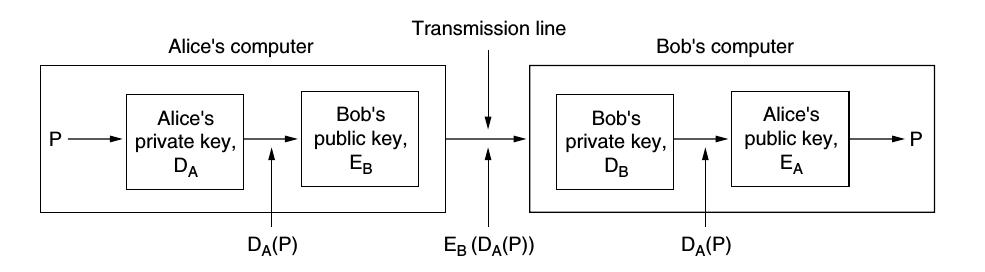
\includegraphics[scale=0.7]{Images/digital_sig_public_key}
\label{fig:dg_key_publickey}
\end{figure}
\textbf{Problems:}
\begin{enumerate}
\item If $D_A$ is changed, then applying old key doesnot lead to message $P$ which is a porblem.
\item If $D_A$ is secret, then Bob can prove any forgery case against him. If $D_A$ is public, then problem arises. 
\end{enumerate}
\textbf{Digital Signature Standard (DSS)} used a variant of El Gamal encrytpion with 1024 bit keys.
\subsection{Message Digests}
Authentication scheme that does not require encrypting the entire message.\\
This scheme is based on the idea of a one-way hash function that takes an arbitrarily long piece of plaintext and from it computes a fixed-length bit string. \\
This hash function, \textit{MD}, often called a message digest, has four important properties:
\begin{enumerate}
\item Given $P$, it is easy to compute $MD(P)$.
\item Given $MD(P)$, it is effectively impossible to find $P$.
\item Given $P$, no one can find $P'$ such that $MD (P') = MD(P)$.
\item A change to the input of even 1 bit produces a very different output.
\end{enumerate}
Message digests save  encryption time and message transport costs.
In the Fig ~\ref{fig:dg_key_publickey}  Instead, of signing $P$ with $K_{BB} (A, t, P)$, BB now computes the message digest by applying MD to $P$, yielding $MD(P)$. BB then encloses $K_{BB} (A, t, MD(P))$ as the fifth item in the list encrypted with KB that is sent to Bob, instead of $K_{BB} (A, t, P)$.\\
In public key cryptosystems: Here, Alice first computes the message digest of her plaintext. She then signs the message digest and sends both the signed digest and the plaintext to Bob. If Trudy replaces P along the way, Bob will see this when he computes $MD(P)$.
\subsubsection{SHA-1 \& SHA-2}
\textbf{SHA}: Secure Hash Algorithm.\\
SHA-1: It processes input data in 512-bit blocks, and it generates a 160-bit message digest. 
\begin{figure}[H]
\caption{SHA-1 algorithm from Alice to Bob}
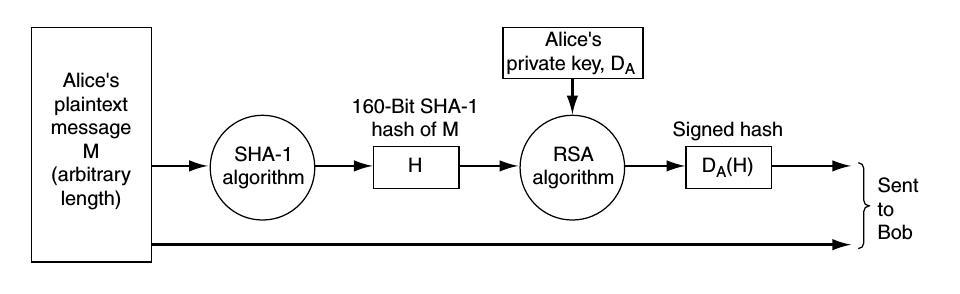
\includegraphics[scale=0.7]{Images/sha1}
\label{fig:sha1}
\end{figure}
After receiving the message, Bob computes the SHA-1 hash himself and also applies Alice’s public key to the signed hash to get the original hash, H. If the two agree, the message is considered valid. Since there is no way for Trudy to modify the (plaintext) message while it is in transit and produce a new one that hashes to H, Bob can easily detect any changes Trudy has made to the message. Used for \textbf{integrity but not secrecy}.\\
\textbf{Working of SHA-1}
\begin{enumerate}
\item  It starts out by padding the message by adding a 1 bit to the end, followed by as many 0 bits as are necessary, but at least 64, to make the length a multiple of 512 bits. 
\item Then a 64-bit number containing the message length before padding is ORed into the low-order 64 bits.
\item During the computation, SHA-1 maintains five 32-bit variables, $H_0$ through $H_4$ , where the hash accumulates. They are initialized to constants specified in the standard.
\item Each of the blocks $M_0$ through $M_{n −1}$ is now processed in turn.
\item For the current block, the 16 words are first copied into the start of an auxiliary 80-word array, W. Then the other 64 words in W are filled in using the formula 
$$W_i = S^1 (W_{i - 3} \text{ XOR } W_{i - 8} \text{ XOR } W_{i -14} \text{ XOR } W_{i -16} )   (16 \le i \le 79)$$
where $S^b(W)$  represents the left circular rotation of the 32-bit word, W, by $b$ bits.
\item Now five scratch variables, A through E, are initialized from $H_0$ through $H_4$ , respectively.
\item The actual calculation can be expressed in pseudo-C as
\begin{minted}[mathescape]{c}
/*for (i = 0; i < 80; i++) {
	temp = $S^5(A) + f_i(B, C, D) + E + W_i + K_i$ ;
	E = D; D = C; C = $S^{30}(B)$; B = A; A = temp;
}*/
\end{minted}
where the $K_i$ constants are defined in the standard. 
\item The mixing functions $f_i$ are defined as \\
$ f_i (B,C,D) = (B \text{ AND } C) OR (\text{ NOT } B \text{ AND } D)$ \hfill $( 0 \le i \le 19) $
$ f_i (B,C,D) = B \text{ XOR } C \text{ XOR } D$ \hfill 
$ (20 \le i \le 39) $
$ f_i (B,C,D) = (B \text{ AND } C) OR (B \text{ AND } D) OR (C \text{ AND } D)$ \hfill 
 $(40 \le i \le 59) $
$ f_i (B,C,D) = B \text{ XOR } C \text{ XOR } D$   \hfill    $(60 \le i \le 79)$
\item When all 80 iterations of the loop are completed, A through E are added to $H_0$ through $H_4$ , respectively.
\item Now that the first 512-bit block has been processed, the next one is started. The W array is reinitialized from the new block, but H is left as it was. 
\item When this block is finished, the next one is started, and so on, until all the 512-bit message blocks have been tossed into the soup. \item When the last block has been finished, the five 32-bit words in the $H$ array are output as the 160-bit cryptographic hash.
\end{enumerate}
New versions of SHA-1 have been developed that produce hashes of 224, 256, 384, and 512 bits. Collectively, these versions are called \textbf{SHA-2}.
\subsubsection{MD5}
\begin{enumerate}
\item The message is padded to a length of 448 bits (modulo 512).
\item Then the original length of the message is appended as a 64-bit integer to give a total input whose length is a multiple of 512 bits.
\item  Each round of the computation takes a 512-bit block of input and mixes it thoroughly with a running 128-bit buffer. 
\item For good measure, the mixing uses a table constructed from the sine function.
\item The point of using a known function is to avoid any suspicion that the designer built in a clever back door through which only he can enter. 
\item This process continues until all the input blocks have been consumed. The contents of the 128-bit buffer form the message digest.
\end{enumerate}
\subsubsection{Birthday Attack}
One might think that it would take on the order of $2^m$ operations to subvert an m-bit message digest. In fact, $2^{\frac{m}{2}}$ operations will often do using the birthday attack. Birthday attack takes a lot of time in computing message digrsts from SHA-1.
\section{Communication Security}
\subsection{Firewalls}
Keeps digital pests \& intruders from using company's LAN. A company can have many LANs connected in arbitrary ways, but all traffic to or from the company is forced through an electronic drawbridge (firewall), as shown in Fig. ~\ref{fig:firewall}. No other route exists.
\begin{figure}[H]
\caption{Firewall Protecting internal network}
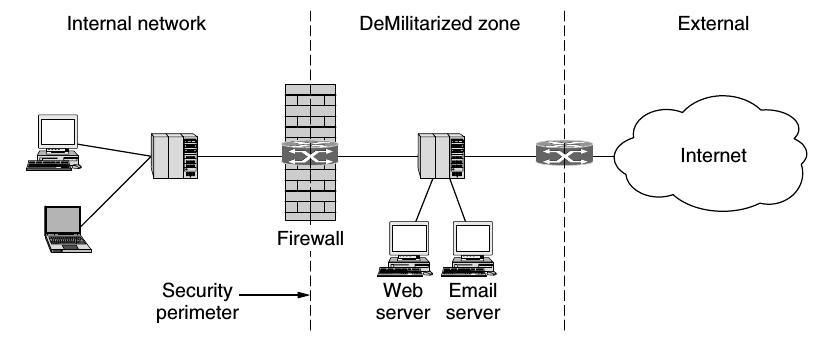
\includegraphics[scale=0.7]{Images/firewall}
\label{fig:firewall}
\end{figure}
The firewall acts as a \textbf{packet filter}. It inspects each and every incoming and outgoing packet. Packets meeting some criterion described in rules formulated by the network administrator are forwarded normally. Those that fail the test are uncermoniously dropped.\\
The filtering criterion is typically given as rules or tables that list sources and destinations that are acceptable, sources and destinations that are blocked, and default rules about what to do with packets coming from or going to other machines.\\
In the common case of a TCP/IP setting, a source or destination might consist of an IP address and a port. Ports indicate which service is desired. \\
The DMZ is the part of the company network that lies outside of the security perimeter. Anything goes here. By placing a machine such as a Web server in the DMZ, computers on the Internet can contact it to browse the company Web site. Now the firewall can be configured to block incoming TCP traffic to port 80 so that computers on the Internet cannot use this port to attack computers on the internal network.\\
 \textbf{Stateful firewalls} map packets to connections and  use TCP/IP header fields to keep track of connections. \\
Another level of sophistication up from stateful processing is for the firewall to implement \textbf{application-level gateways}.\\
Looking inside packets, beyond even the TCP header, to see what the application is doing. With this capability, it is possible to distinguish HTTP traffic used for Web browsing from HTTP traffic used for peer-to-peer file sharing. \\
Firewalls cannot prevent \textbf{Denial of Service} attacks, where an intruder sends thoudsands of req. after establishing connection to bring own the web server.
\chapter{Application Layer}
\section{DNS - Domain Name System}
The essence of DNS is the invention of a hierarchical, domain-based naming scheme and a distributed database system for implementing this naming scheme. It is \textit{primarily used for mapping host names to IP addresses} but can also be used for other purposes. \\
\begin{enumerate}
\item To map a name onto an IP address, an application program calls a library procedure called the resolver, passing it the name as a parameter. 
\item The resolver sends a query containing the name to a local DNS server, which looks up the name and returns a response containing the IP address to the resolver, which then returns it to the caller. 
\item The query and response messages are sent as UDP packets.
\item Armed with the IP address, the program can then establish a TCP connection with the host or send it UDP packets.
\end{enumerate}
\textbf{DNS Name Space:}\\
\begin{minipage}{0.5\textwidth}
\centering
\captionof{figure}{A portion of the Internet domain name space}
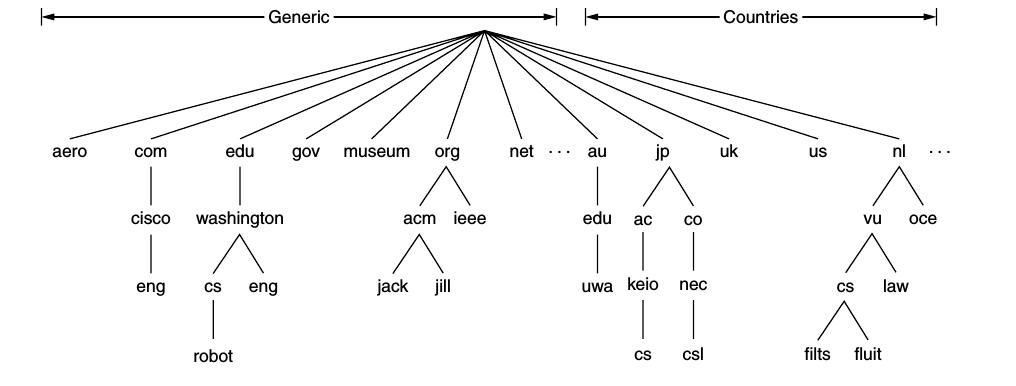
\includegraphics[width=\textwidth,height=0.7\textwidth]{Images/dnsnamespace}
\label{fig:dns}
\end{minipage}
\begin{minipage}{0.5\textwidth}
\centering
\captionof{figure}{Domain Name Space mapped to zones}
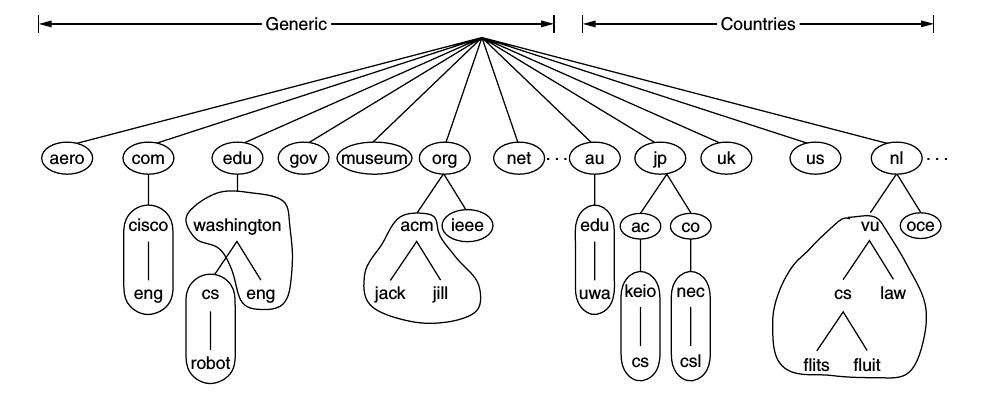
\includegraphics[width=\textwidth,height=0.7\textwidth]{Images/dnszones}
\label{fig:dnszones}
\end{minipage}
Each domain is named by the path upward from it to the (unnamed) root. The components are separated by periods. Thus, the engineering department at Cisco might be eng.cisco.com., rather than a UNIX -style name such as /com/cisco/eng. Notice that this hierarchical naming means that eng.cisco.com. does not conflict with a potential use of eng in eng.washington.edu., which might be used by the English department at the University of Washington.\\
\textbf{Domain Names}: absolute or relative, case-insensitive . \\
\textbf{Domain Resource Records}: Every domain, whether it is a single host or a top-level domain, can have a set of resource records associated with it. These records are the DNS database.\\
The primary function of DNS is to map domain names onto resource
records. A resource record is a five-tuple.
\begin{verbatim}
Domain_name     Time_to_live     Class     Type    Value
\end{verbatim}
\begin{enumerate}
\item \textbf{Domain name}  Tells the domain to which this record applies. Primary Key
\item \textbf{Time to live} Field gives an indication of how stable the record is. Seconds
\item \textbf{Class}  For Internet information, it is always IN. For non-Internet information, other codes can be used, but in practice these are rarely seen.
\item \textbf{Type}  Tells what kind of record this is.
\item \textbf{Value} This field can be a number, a domain name,
or an ASCII string. The semantics depend on the record type. 
\end{enumerate}
\begin{figure}[H]
\caption{DNS Resource Records Types}
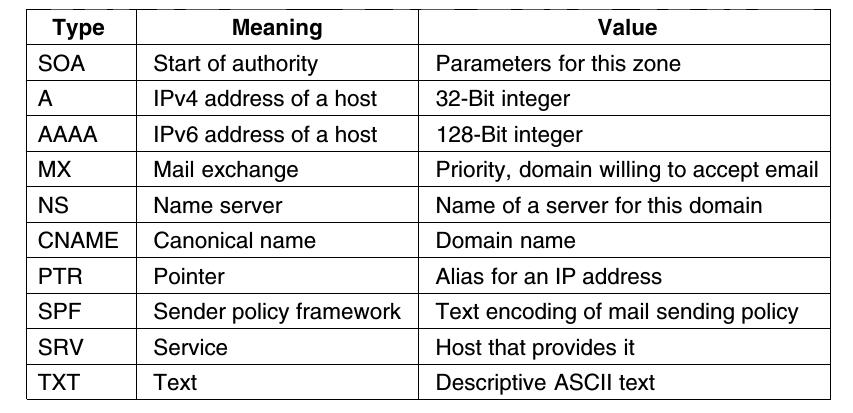
\includegraphics[scale=0.7]{Images/dnsresrec}
\label{fig:dns_res_rec}
\end{figure}
\subsection{Name Servers}
A single name server could contain the entire DNS database
and respond to all queries about it.  The DNS name space is divided into nonoverlapping zones. Where the zone boundaries are placed within a zone is up to that zone's administrator. 
\section{HTTP - Hyper Text Transfer Protocol}
 Used to transport all this information between Web servers and clients. HTTP is a simple request-response protocol that normally runs over TCP. It  specifies what messages clients may send to servers and what responses they get  back in return.\\
 The request and response headers are given in ASCII, just like in
SMTP. The contents are given in a MIME-like format, also like in SMTP. 
\textbf{Default Port:} 80.\\
\textbf{HTTP 1.0} After the connection was established a sin-\\
gle request was sent over and a single response was sent back.
\textbf{HTTP 1.1}
\begin{figure}[H]
\caption{HTTP 1.1 with (a) multiple connections and sequential requests. (b)A persistent connection and sequential requests. (c) A persistent connection and pipelined requests. }
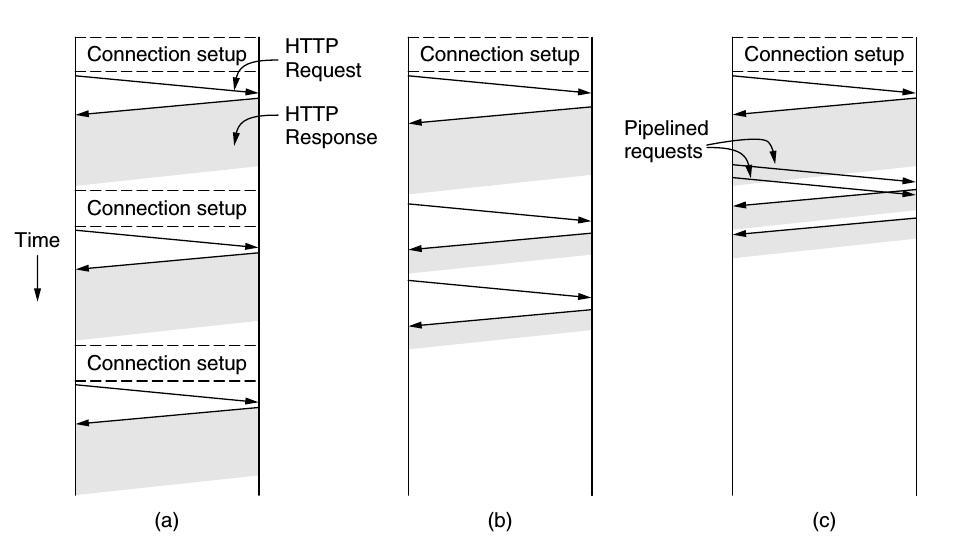
\includegraphics[scale=0.5]{Images/httpreq}
\label{fig:http_req}
\end{figure}
\chapter{Routing Algorithms}
\section{Introduction}
\begin{enumerate}
\item The \textbf{routing algorithm} is that part of the \textbf{network layer} software responsible for deciding which output line an incoming packet should be transmitted on. 
\item If the network uses datagrams internally, this decision must be made anew for every arriving data packet since the best route may have changed since last time. 
\item If the network uses virtual circuits internally, routing decisions are made only when a new virtual circuit is being set up. (\textbf{Session Routing})
\item Difference between routing \& forwarding: \textbf{Routing - } making the decision which routes to use (filling \& updating routing tables). \textbf{Forwarding -}  handles each packet as it arrives, looking up the outgoing line to use for it in the routing tables.
\item Desirable in a routing algorithm: correctness, simplicity, robustness, stability, fairness, and efficiency.
\item Desired: Minimizing the mean packet delay, maximizing total network throughput.
\item Routing algorithms can be grouped into two major classes: nonadaptive and adaptive. 
\begin{enumerate}
\item Non Adaptive: Static Routing
\item Adaptive: Dynamic Routing
\end{enumerate}
\item \textbf{Optimality Principle}: It states that if router J is on the optimal path from router I to router K, then the optimal path from J to K also falls along the same route. 
\item The set of optimal routes from all sources to a given destination form a tree rooted at the destination. Such a tree is called a \textbf{sink tree}.
\item DAG - Directed Acyclic Graphs. No Loops.
\end{enumerate}
\section{Shortest Path Algorithm - Dijsktra}
\begin{algorithm}[H]
\caption{Calculate the shortest path from source node to all destination nodes}
\label{fig:cn_sh_pt_algo}
\begin{algorithmic}[1]
\REQUIRE A weighted undirected graph with source node and non-negative weights
\ENSURE Shortest path between source node and all other nodes
\STATE Source node labelled(permanent : path fixed)
\STATE Other nodes unalbelled(temporary : path not fixed)
\STATE Node labelling $\leftarrow$ ($\infty, -$) : represents predecessor in shortest path route.
\WHILE{All nodes are not visited}
\WHILE{All adjacent nodes are not visited}
\STATE dist. $\leftarrow$ distance between previous node and visited node.
\STATE pred. $\leftarrow$ Previous node
\STATE Mark visited nodes with as(dist., pred.)
\ENDWHILE
\STATE Mark remaining nodes as ($\infty, -$)
\STATE Mark the smallest dist. node as permanent
\ENDWHILE
\end{algorithmic}
\end{algorithm}
\begin{figure}[H]
\caption{Sample run of Dijsktra's Algorithm}
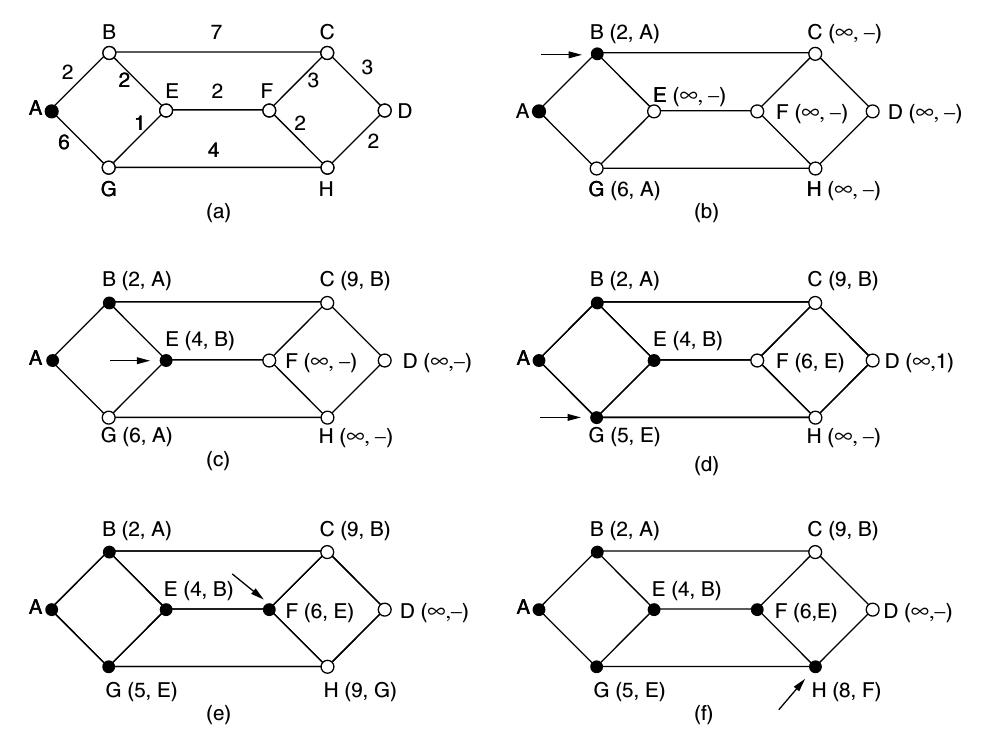
\includegraphics[scale=0.6]{Images/dijsktra_algo}
\label{fig:cn_dijsktra_algo}
\end{figure}
\section{Flooding}
\begin{enumerate}
\item Every incoming packet is sent out on every outgoing line except the one it arrived on.
\item Measures to prevent duplication:
\begin{enumerate}
\item  \textbf{Hop counter} contained in the header of each packet that is decremented at each hop, with the packet being discarded when the counter reaches zero. Ideally, the hop counter should be initialized to the length of the path from source to destination.
\item  Have routers keep track of which packets have been flooded, to avoid sending them out a second time. One
way to achieve this goal is to have the source router put a \textbf{sequence number} in each packet it receives from its hosts. 
\end{enumerate}
\end{enumerate}
\section{Distance Vector Routing - Bellman Ford}
A \textbf{distance vector routing algorithm} operates by having each router maintain a table (i.e., a vector) giving the best known distance to each destination and which link to use to get there.  These tables are updated by exchanging information with the neighbors. Eventually, every router knows the best link to reach each destination.
\begin{algorithm}[H]
\caption{Calculate the shortest path from source node to all destination nodes}
\label{fig:cn_dis_vt_algo}
\begin{algorithmic}[1]
\REQUIRE A weighted undirected graph with source node and non-negative weights
\ENSURE Shortest path between any node and any nodes
\STATE shortestPath[n][n] $\leftarrow$ Vector table containing shortest distances from $V_i$ to $V_j$
\STATE distArray[n][n] $\leftarrow$ distance array containing distance between distance between any node to any node
\STATE distArray[i][j] $\leftarrow$ distance between $V_i$ \& $V_j$.
\STATE delay[n][n] $\leftarrow$ delay from any node to its neighbour nodes.
\STATE delay[i][j] $\leftarrow$ delay from $V_i$ to $V_j$. - if not a neighbour. $k \in \mathrm{W}$ if neighbour.
\WHILE{all nodes are not visited}
\STATE $V_i \leftarrow$ visited, adj = 0 
\FOR{All nodes $V_j$ adjacent to $V_i$}
\STATE Calculate delay[i][j]
\STATE adj++
\ENDFOR
\STATE paths[adj] = {0}
\FOR {All nodes $V_k$}
\FOR {All nodes $V_j$ adjacent to $V_i$}
\STATE paths[j] = delay[i][j] + distArray[j][k];
\ENDFOR
\STATE min $\leftarrow$ minimum value in  paths[].
\STATE shortestPath[i][k] = min
\ENDFOR
\ENDWHILE
\end{algorithmic}
\end{algorithm}
\begin{figure}[H]
\caption{Sample run of Bellman Ford's Algorithm}
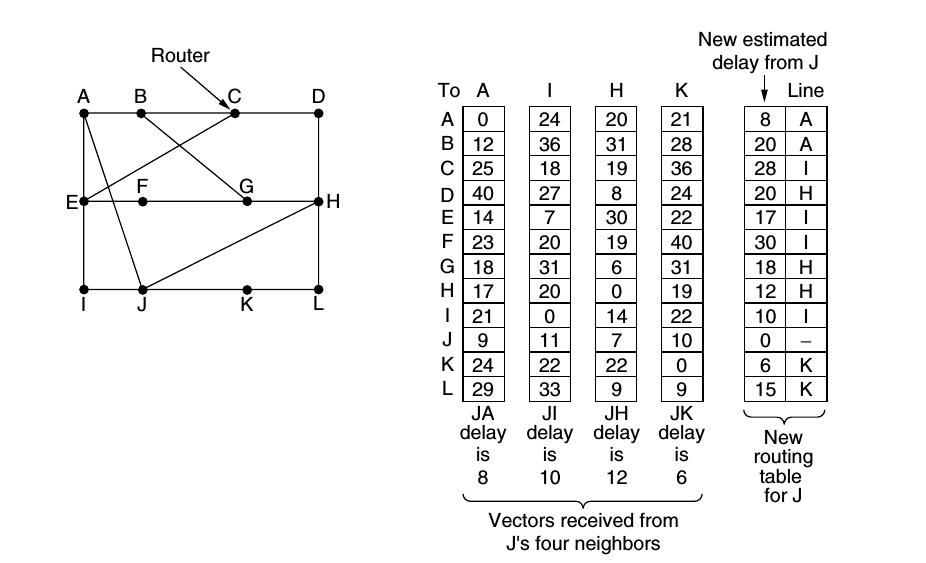
\includegraphics[scale=0.6]{Images/bellman_algo}
\label{fig:cn_bellman_algo}
\end{figure}
\textbf{Count to infinity Problem:} The settling of routes to best paths across the network is called \textbf{convergence}.
\section{Link State Routing}
Variants of link state routing called \textbf{IS-IS  (Intermediate System-Intermediate System)} and \textbf{OSPF (Open Shortest Path First)}. \\
Each router must do the following things to make it work:
\begin{enumerate}
\item Discover its neighbors and learn their network addresses.
\item Set the distance or cost metric to each of its neighbors.
\item Construct a packet telling all it has just learned.
\item Send this packet to and receive packets from all other routers.
\item Compute the shortest path to every other router.
\end{enumerate}
In effect, the complete topology is distributed to every router. Then Dijkstra’s algorithm can be run at each router to find the shortest path to every other router. Compared to distance vector routing, link state routing requires more memory and computation. But no problem of slow convergence as in distance vector routing.
\subsection{Learning abput neighbours}
Sending a special HELLO packet on each point-to-point line. The router on the other end is expected to send back a reply giving its name.  A better way to model the LAN connecting different routers is to consider it as a node itself.
\subsection{Setting Link Costs}
 A common choice is to make the cost inversely proportional to the bandwidth of the link. For example, 1-Gbps Ethernet may have a cost of 1 and 100-Mbps Ethernet a cost of 10. This makes higher-capacity paths better choices. Ig routers geogfraphoically spread, then delay could be link cost.
\subsection{Building Link State Packets}
One possibility is to build them periodically, that is, at regular intervals. Another possibility is to build them when some significant event occurs, such as a line or neighbor going down or coming back up again or changing its properties appreciably.
\begin{figure}[H]
\caption{Link Sate Packets}
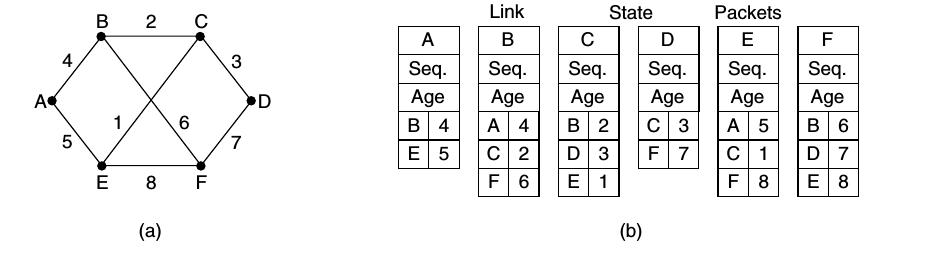
\includegraphics[scale=0.6]{Images/linkStatePkt}
\label{fig:cn_link_st_pkt}
\end{figure}
\subsection{Distributing the Link State Packets}
All of the routers must get all of the link state packets quickly and reliably. 
\subsubsection{Fundamental Idea}
Use flooding to distribute the link state packets to all routers.  To keep the flood in check, each packet contains a sequence number that is incremented for each new packet sent. Routers keep track of all the (source router, sequence) pairs they see. When a new link state
packet comes in, it is checked against the list of packets already seen. If it is new, it is forwarded on all lines except the one it arrived on. If it is a duplicate, it is discarded.
\subsubsection{Problems}
\begin{enumerate}
\item Wrap around of sequence numbers: \textbf{Solution} - Use 32 bit seq. numbers.
\item If a router ever crashes, it will lose track of its sequence number.
\item If a sequence number is ever corrupted and 65,540 is received instead of 4 (a 1-bit error), packets 5 through 65,540 will be rejected as obsolete, since the current sequence number will be thought to be 65,540. \textbf{Solution:} include age of packet amd decrement it once per second.
\end{enumerate}
 The send flags mean that the packet must be sent on the indicated link. The acknowledgement flags mean that it must be acknowledged there.  The situation with the third packet, from E, is different. It arrives  twice, once via EAB and once via EFB. Consequently, it has to be sent only to C  but must be acknowledged to both A and F, as indicated by the bits.\\
 If a duplicate arrives while the original is still in the buffer, bits have to be  changed. For example, if a copy of C’s state arrives from F before the fourth  entry in the table has been forwarded, the six bits will be changed to 100011 to in-  dicate that the packet must be acknowledged to F but not sent there.
\begin{figure}[H]
\caption{Packet Buffer for Router B}
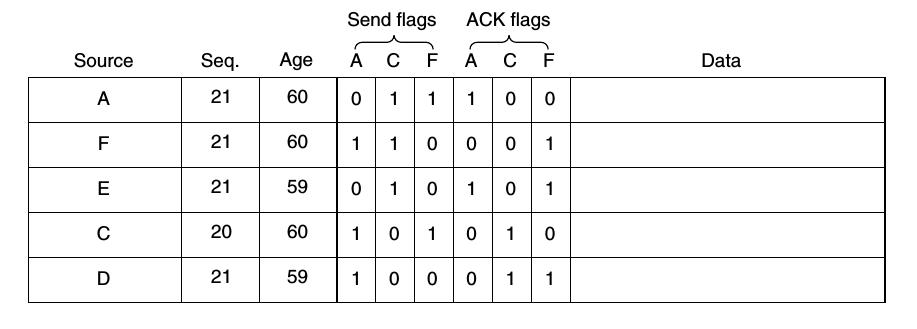
\includegraphics[scale=0.6]{Images/packet-buffer}
\label{fig: cn_lsp}
\end{figure} 
\subsection{Computing Shortest Path}
 Every link in the newtwork graph is, in fact, represented twice, once for each direction.Dijkstra's algorithm can be run locally to construct the shortest paths to all possible destinations. The results of this algorithm tell the router which link to use to reach each destination. This information is installed in the routing tables, and normal operation is resumed.
\todo{Use a 32-bit sequence number. With one link state packet per second, it would take 137 years to wrap around. Time = $\dfrac{2^{\text{no. of bits}}}{BW }$. Here BW = 1lsp/sec. no. of bits = 32}
\section{Hierarchial Routing}
When hierarchical routing is used, the routers are divided into what we will call regions. Each router knows all the details about how to route packets to destinations within its own region but knows nothing about the internal structure of other regions. For huge networks, a two-level hierarchy may be insufficient; it may be necessary to group the regions into clusters, the clusters into zones, the zones into groups, and so on.
\begin{figure}[H]
\caption{Hierarchial Routing}
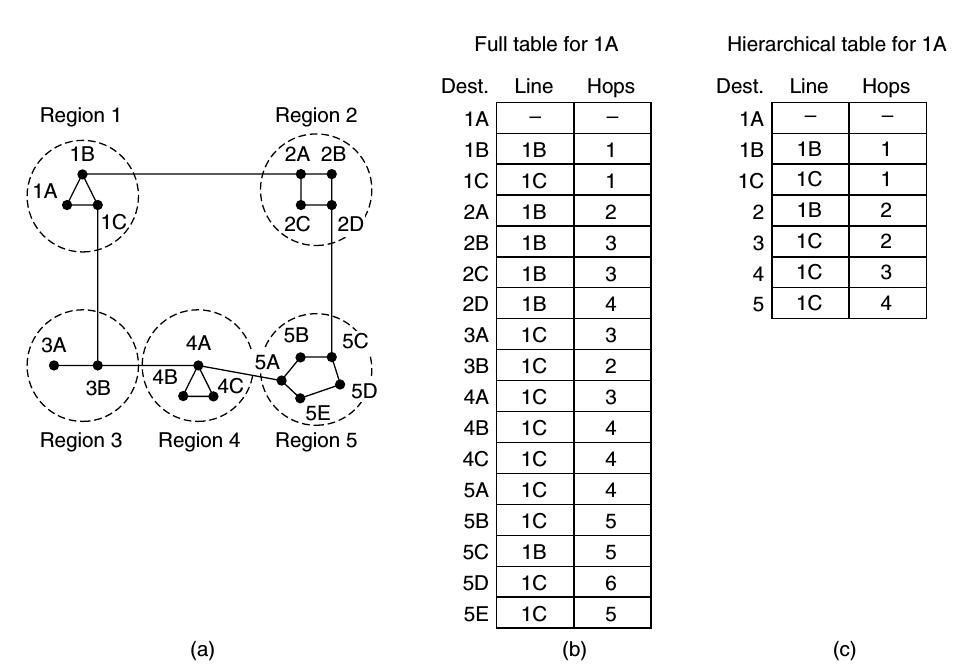
\includegraphics[scale=0.6]{Images/hierar_rout}
\label{fig:cn_hie_rout}
\end{figure}
 For example, consider a network with 720 routers. If there is no hierarchy, each router needs 720 routing table entries. If the network is partitioned into 24 regions of 30 routers each, each router needs 30 local entries plus 23 remote entries for a total of 53 entries. If a three-level hierarchy is chosen, with 8 clusters each containing 9 regions of 10 routers, each router needs 10 entries for local routers, 8 entries for routing to other regions within its own cluster, and 7 entries for distant clusters, for a total of 25 entries. Optimal no. of levels in N routers is $\ln N$ making total of $e \ln N$ no. of entries per router.
\section{Broadcast Routing}
Sending a packet to all destinations simultaneously is called \textbf{broadcasting}.  The network bandwidth is therefore used more efficiently.\\
\textbf{Problems:} Source to know all the destinations, Router to determine where to send one multidestination packet as it is for multiple distinct packets.\\
\textbf{Better broadcast routing technique:} Flooding. When implemented with a sequence number per source, flooding uses links efficiently
with a decision rule at routers.\\
\textbf{Reverse path forwarding:} \todo{did not understand}
\textbf{Spanning tree Algorithm:}  A spanning tree is a subset of the network that includes all the routers but contains no loops. Sink trees are spanning trees. If each router knows which of its lines belong to the spanning tree, it can copy an incoming broadcast packet onto all the spanning tree lines except the one it arrived on. This method makes excellent use of bandwidth, generating the absolute minimum number of packets necessary to do the job. 
\section{Multicast Routing}
Sending a message to such a group is called multicasting, and the routing algorithm used is called \textbf{multicast routing}. All multicasting schemes require some way to create and destroy groups and to identify which routers are members of a group.\\
Multicast routing schemes build on the broadcast routing schemes we have already studied, sending packets along spanning trees to deliver the packets to the members of the group while making efficient use of bandwidth. \\
Types of pruning spanning trees:
\begin{enumerate}
\item  \textbf{MOSPF (Multicast OSPF)}
\begin{enumerate}
\item If \textbf{link state routing} is used and each router is aware of the complete topology, including which hosts belong to which groups.
\item Each router can then construct its own pruned spanning tree for each sender to the group in question by constructing a sink tree for the sender as usual and then removing all links that do not connect group members to the sink node. 
\end{enumerate}
\item  \textbf{DVMRP (Distance Vector Multicast Routing Protocol) }
\begin{enumerate}
\item With \textbf{distance vector routing}, a different pruning strategy can be followed.
\item The basic algorithm is \textbf{reverse path forwarding}. However, whenever a router with no hosts interested in a particular group and no connections to other routers receives a multicast message for that group, it responds with a PRUNE message, telling the neighbor that sent the message not to send it any more multicasts from the sender for that group.
\item When a router with no group members among its own hosts has received such messages on all the lines to which it sends the multicast, it, too, can respond with a PRUNE message.
\end{enumerate}
\end{enumerate}
\section{IPv4 - Network Layer}
\subsection{Communication in Internet}
 The transport layer takes data streams and breaks them up so that they may be sent as IP packets. In theory, packets can be up to 64 KB each, but in practice they are usually not more than 1500 bytes (so they fit in one Ethernet frame). IP routers forward each packet through the Internet, along a path from one router to the next, until the destination is reached. At the destination, the network layer hands the data to the transport layer, which gives it to the receiving process. When all the pieces finally get to the destination machine, they are reassembled by the network layer into the original datagram. This datagram is then handed to the transport layer.
\begin{figure}[H]
\caption{IPv4 Header}
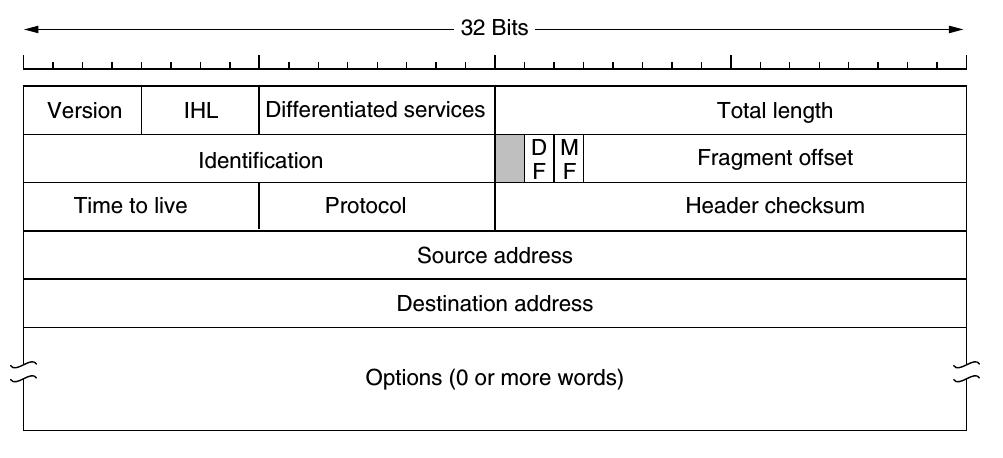
\includegraphics[scale=0.8]{Images/ipv4header}
\label{fig:cn_ipv4}
\end{figure}
\chapter{Error \& Flow control - Data Link Layer}
\section{Introduction}
The data link layer uses the services of the physical layer to send and receive bits over communication channels. It has a number of functions, including:
\begin{enumerate}
\item Providing a well-defined service interface to the network layer.
\item Dealing with transmission errors.
\item Regulating the flow of data so that slow receivers are not swamped by fast senders.
\end{enumerate}
4 methods to \textbf{break bit streams into frames}:
\begin{enumerate}
\item Byte count.
\item Flag bytes with byte stuffing.
\item Flag bits with bit stuffing.
\end{enumerate}
\subsection{Byte Count}
A field in the header to specify the number of bytes in the frame. When the data link layer at the destination sees the byte count, it knows how many bytes follow and hence where the end of the frame is.
\begin{figure}[H]
\caption{Byte Count  (a) Without errors. (b) With one error.}
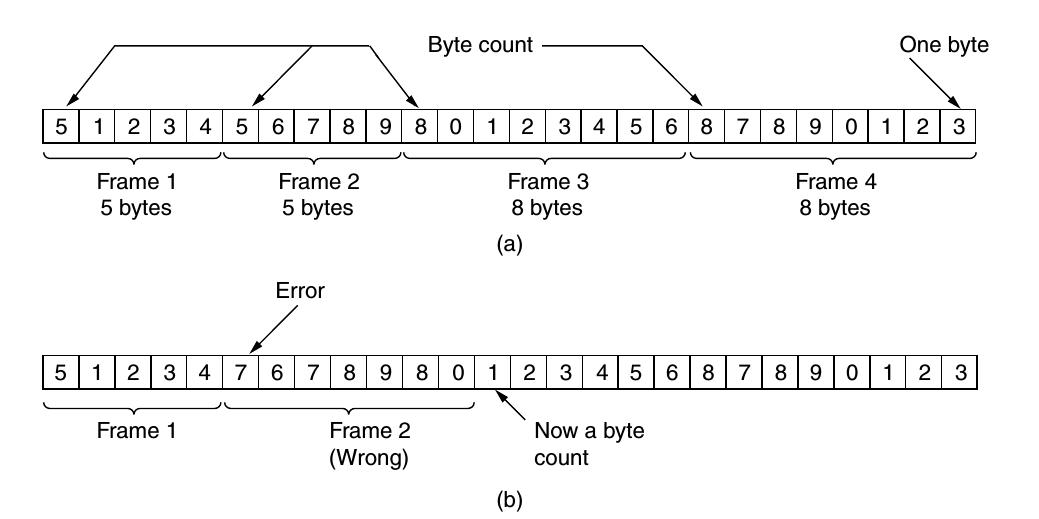
\includegraphics[scale=0.6]{Images/byte_count}
\label{fig:cn_byte_count}
\end{figure}
\subsection{Byte Stuffing}
\begin{enumerate}
\item Add \textbf{FLAG} byte at the start and end of each frame. Two consecutive flag bytes indicate the end of one frame and the start of the next. 
\item If \textbf{FLAG} byte in data of the frame, then add \textbf{ESC} byte to the before of \textbf{FLAG} byte.
\item If \textbf{ESC} occurs in th e middle of the data,  then stuff it with an \textbf{ESC} byte.
\end{enumerate}
Byte Stuffing is used in PPP(Point to Point Protocol).
\begin{figure}[H]
\caption{Byte Stuffing  (a) A frame delimited by flag bytes. (b) Four examples of byte sequences before and after byte stuffing.}
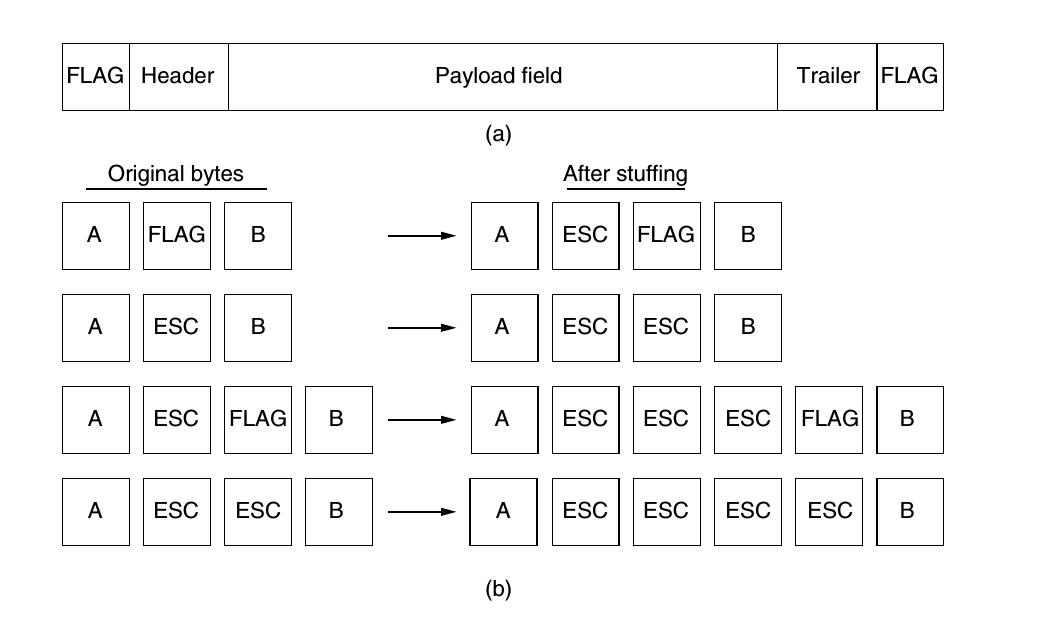
\includegraphics[scale=0.6]{Images/byte_stuffing}
\label{fig:cn_byte_stuff}
\end{figure}
\subsection{Bit Stuffing}
Used in HDLC(High-level Data Link Control).
\begin{enumerate}
\item Each frame begins and ends with a special bit pattern, 01111110 or 0x7E in hexadecimal.  - FLAG Byte.
\item  Whenever the sender's data link layer encounters five consecutive 1s in the data, it automatically stuffs a 0 bit into the outgoing bit stream - ESC Byte.
\item When the receiver sees five consecutive incoming 1 bits, followed by a 0 bit, it automatically destuffs (i.e., deletes) the 0 bit.
\end{enumerate}
\todo{Suppose 111110 is in data, does receiver destuff that leading to wrong information (in Bit Stuffing)?}
\begin{figure}[H]
\caption{Bit Stuffing  (a) The original data. (b) The data as they appear on the line. (c) The data as they are stored in the receiver's memory after destuffing.}
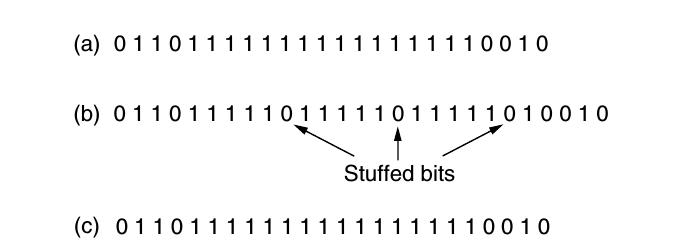
\includegraphics[scale=0.6]{Images/bit_stuffing}
\label{fig:cn_bit_stuff}
\end{figure}
\section{Error Correction \& Detection}
\subsection{Error Correcting Codes}
\begin{enumerate}
\item Hamming codes.
\item Binary convolutional codes.
\item Reed-Solomon codes.
\item Low-Density Parity Check codes.
\end{enumerate}
In a \textbf{systematic code}, the $m$ data bits are sent directly, along with the check bits, rather than being encoded themselves before they are sent. In a \textbf{linear code}, the $r$ check bits are computed as a linear function of the $m$ data bits. 
\begin{definition}[Codeword]
A frame generally consists of $m$ data bits (message) and $r$ code (redundant/check) bits to form an n bit codeword where $n=m+r$.
\end{definition}
\subsubsection{Hamming Codes}
\begin{definition}[Hamming distance]
 The number of different digits $d(x, y)$ between two codewords $x$ and $y$. For example, 000 and 111 have a Hamming distance of 3.
\end{definition}
\begin{definition}[Coderate]
The fraction of the codeword that carries information that is not redundant, or $\dfrac{m}{n}$.
\end{definition}
\begin{definition}[Even Parity]
In the case of even parity, \textbf{the number of bits whose value is 1 in a given set are counted.} If that total is odd, the parity bit value is set to 1, making the total count of 1's in the set an even number. If the count of ones in a given set of bits is already even, the parity bit's value remains 0.
\end{definition}
\begin{definition}[Odd Parity]
In the case of odd parity, the situation is reversed. Instead, if the sum of bits with a value of 1 is odd, the parity bit's value is set to zero. And if the sum of bits with a value of 1 is even, the parity bit value is set to 1, making the total count of 1's in the set an odd number.
\end{definition}
If two codewords are a Hamming distance $d$ apart, it will require $d$ single-bit errors to convert one into the other.
To reliably detect $d$ errors, you need a distance $d + 1$ code because with such a code there is no way that $d$ single-bit errors can change a valid codeword into another valid codeword. To correct $d$ errors, you need a distance $2d + 1$ code because that way the legal codewords are so far apart that even with $d$ changes the original codeword is still closer than any other codeword. 
Number of check bits needed to correct single errors: $(m + r + 1) \le 2^r$.\\
The bits that are powers of 2 (1, 2, 4, 8, 16, etc.) are check bits. The rest (3, 5, 6, 7, 9, etc.) are filled up with the m data bits. This construction gives a code with a Hamming distance of 3 (11 = 1 + 2 + 8. max 3 numbers), which means that it can correct single errors (or detect double errors). \\
\textbf{Example}: Message - 1000001. To compute  check bits: express rest of bits in as a summation of check bits. ex., 11 = 1 + 2 + 8. No. of 2's in expanded sum gives the parity for 2 in new message.
Sent Message: 0 0 1 0 0 0 0 1 0 0 1, Received Mwssage:  0 0 1 0 1 0 0 1 0 0 1.\\
Check bits should be computed including check bits: $1: 1, 2: 0, 4: 1, 8: 0$. Recheck parity bits: $1: 1, 2: 0, 4: 1, 8: 1$. A single-bit error occurred on the channel so the check results are 0, 1, 0, and 1 for k = 8, 4, 2, and 1. Parity bits of 4 and 1 are changed. Therefore, bit $4+1 = 5$ should be flipped.
\begin{figure}[H]
\caption{Hamming Codes for (11, 7) for even parity}
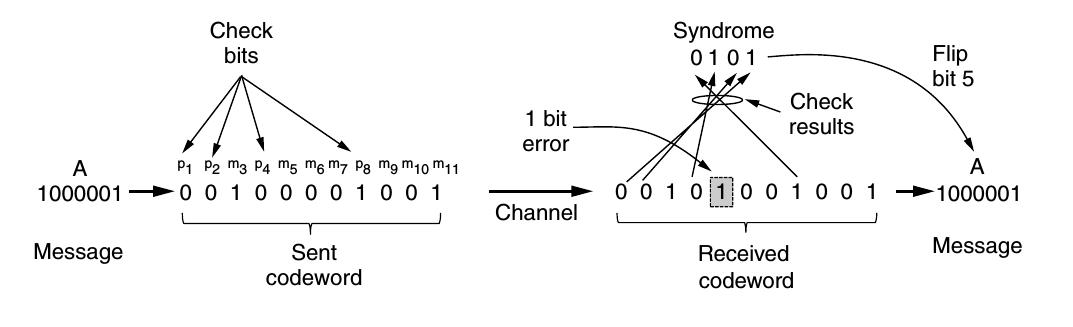
\includegraphics[scale=0.6]{Images/hammingcodes}
\label{fig:cn_hamming_codes}
\end{figure}
\subsubsection{Convolution Codes}
Not a block code. An encoder processes a sequence of input bits and generates a sequence of output bits. Output depends on current and previous input bits(memory). The number of previous bits on which the output depends is called the constraint length of the code.
\begin{figure}[H]
\caption{Convolution Codes}
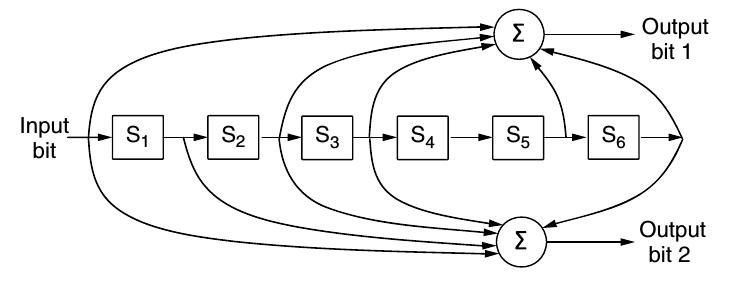
\includegraphics[scale=0.6]{Images/convolutioncodes}
\label{fig:cn_convolu_code}
\end{figure}
\subsubsection{Reed Solomon Codes}
Reed-Solomon codes are linear block codes. Reed-Solomon codes are based on the fact that every $n$ degree polynomial is uniquely determined by $n + 1$ points. we have two data points that represent a line and we send those two data points plus two check points chosen to lie on the same line. If one of the points is received in error, we can still recover the data points by fitting a line to the received points. Three of the points will lie on the line, and one point, the one in error, will not. By finding the line we have corrected the error. \\
For $m$ bit symbols, the codewords are $2^m - 1$ symbols long. A popular choice is to make $m = 8$ so that symbols are bytes. A codeword is then 255 bytes long. The (255, 233) code is widely used; it adds 32 redundant symbols to 233 data symbols. \\
They are based on m bit symbols, a single-bit error and an m-bit burst error are both treated simply as one symbol error. When $2t$ redundant symbols are added, a Reed-Solomon code is able to correct up to $t$ errors in any of the transmitted symbols. This means, for example, that the (255, 233) code, which has 32 redundant symbols, can correct up to 16 symbol errors. Since the symbols may be consecutive and they are each 8 bits, an error burst of up to 128 bits can be corrected.
\subsection{Error Detecting Codes}
\begin{enumerate}
\item Parity.
\item Checksums.
\item Cyclic Redundancy Checks (CRCs).
\end{enumerate}
\subsubsection{Parity}
A single parity bit is appended to the data. The parity bit is chosen so that the number of 1 bits in the codeword is even (or odd). 
For example, when 1011010 is sent in even parity, a bit is added to the end to make it 10110100. With odd parity 1011010 becomes
10110101. A code with a single parity bit has a distance of 2, since any single-bit error produces a codeword with the wrong parity. This means that it can detect single-bit errors.
\begin{figure}[H]
\caption{Interleaving parity}
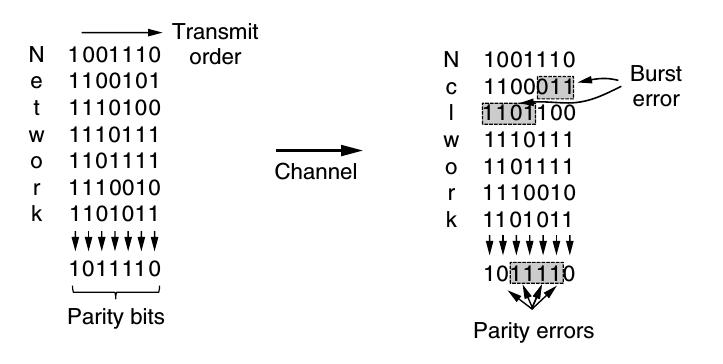
\includegraphics[scale=0.6]{Images/interleavingparity}
\label{fig:cn_inter_parity}
\end{figure}
\subsubsection{Checksums}
The checksum is usually placed at the end of the message, as the complement of the sum function. This way, errors may be detected by summing the entire received codeword, both data bits and checksum. If the result comes out to be zero, no error has been detected.
\todo{How to calculate and detect errors in checksum?}
\subsubsection{CRC(Cyclic Redundancy Check)}
For example, 110001 has 6 bits and thus represents a six-term polynomial with coefficients 1, 1, 0, 0, 0, and 1: $1x^5 + 1x^4 + 0x^3 + 0x^2 + 0x^1 + 1x^0$. Addition and substraction in XOR format.\\
When the polynomial code method is employed, the sender and receiver must agree upon a generator polynomial, $G(x)$, in advance. Both the high and low-order bits of the generator must be 1. To compute the CRC for some frame with m bits corresponding to the polynomial $M(x)$, the frame must be longer than the generator polynomial. The idea is to append a CRC to the end of the frame in
such a way that the polynomial represented by the checksummed frame is divisible by $G(x)$. When the receiver gets the checksummed frame, it tries dividing it by $G(x)$. If there is a remainder, there has been a transmission error.
\begin{enumerate}
\item Let $r$ be the degree of $G(x)$. Append $r$ zero bits to the low-order end of the frame so it now contains $m + r$ bits and corresponds to the polynomial $x^rM(x)$.
\item Divide the bit string corresponding to $G(x)$ into the bit string corresponding to $x^rM(x)$, using modulo 2 division.
\item Subtract the remainder (which is always $r$ or fewer bits) from the bit string corresponding to $x^rM(x)$ using modulo 2 subtraction. The result is the checksummed frame to be transmitted. Call its polynomial $T(x)$.
\end{enumerate}
\todo{How are error detected in CRC?}
\begin{figure}[H]
\caption{Calculating CRC}
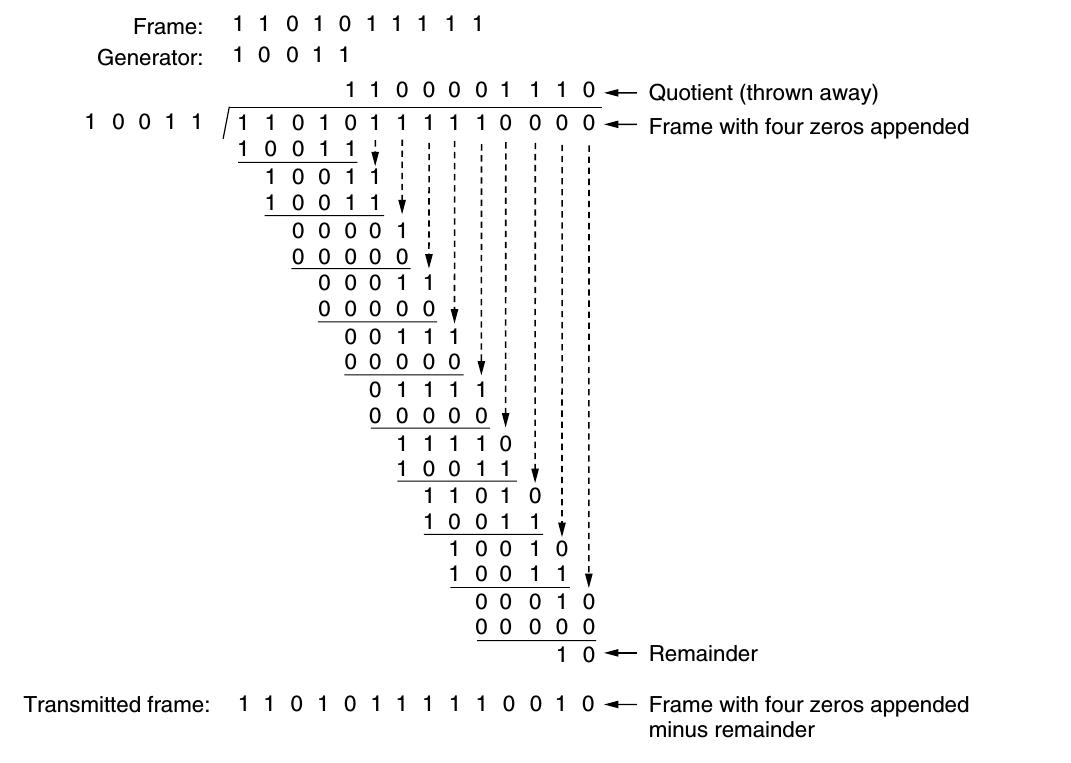
\includegraphics[scale=0.6]{Images/crc}
\label{fig:cn_crc}
\end{figure}
\section{Data Link Protocols}
\subsection{Simplex Protocol}
\textbf{Assumptions}: Error free flow of information, simplex protocol.
\textbf{Sender}: The sender in data link layer receives packet fom the network layer of sender. The data link layer breaks the packets into frames and passes onto the receiver in the data link layer.
\textbf{Receiver}: The receiver receives the frames from the sender of data link layer. It then passes it to network layer of receiver and waits foor other frames..
\subsection{Stop \& Wait Protocol for Error free}
Preventing the sender from flooding the receiver with frames faster than the latter is able to process them. After having passed a packet to its network layer, the receiver sends a little dummy frame back to the sender which, in effect, gives the sender permission to transmit the next frame. After having sent a frame, the sender is required by the protocol to bide its time until the little dummy (i.e., acknowledgement) frame arrives.
\subsection{Stop \& Wait Protocol for Noisy Channel}
\textbf{Example}: ARQ (Automatic Repeat reQuest)
\subsection{Sliding Window Protocols}
\textbf{Piggybacking}: Sender of data link layer sends frames to data link layer of receiver and starts timer for acknowledgement to come. After receiving the frame, instead of sending acknowledgement the receiver waits for packet from network layer and attaches the ack to it and sends it to the sender of dll. If n/w layer doesn't send any packet ack frame is sent separately. Use of sequence nos. to avoid duplication. Use of kind field in header to find out if frame is data or control(ack) in full-duplex channel(two way communication).\\
The sender maintains a set of sequence numbers corresponding to frames it is permitted to send. These frames are said to fall within the sending window. Similarly, the receiver also maintains a receiving window corresponding to the set of frames it is permitted to accept.\\
The sequence numbers within the sender's window represent frames that have been sent or can be sent but are as yet not acknowledged. Whenever a new packet arrives from the network layer, it is given the next highest sequence number, and the upper edge of the window is advanced by one. When an acknowledgement comes in, the lower edge is advanced by one. In this way the window continuously maintains a list of unacknowledged frames.
\begin{figure}[H]
\caption{A sliding window of size 1, with a 3-bit sequence number. (a) Initially. (b) After the first frame has been sent. (c) After the first frame has been received. (d) After the first acknowledgement has been received.}
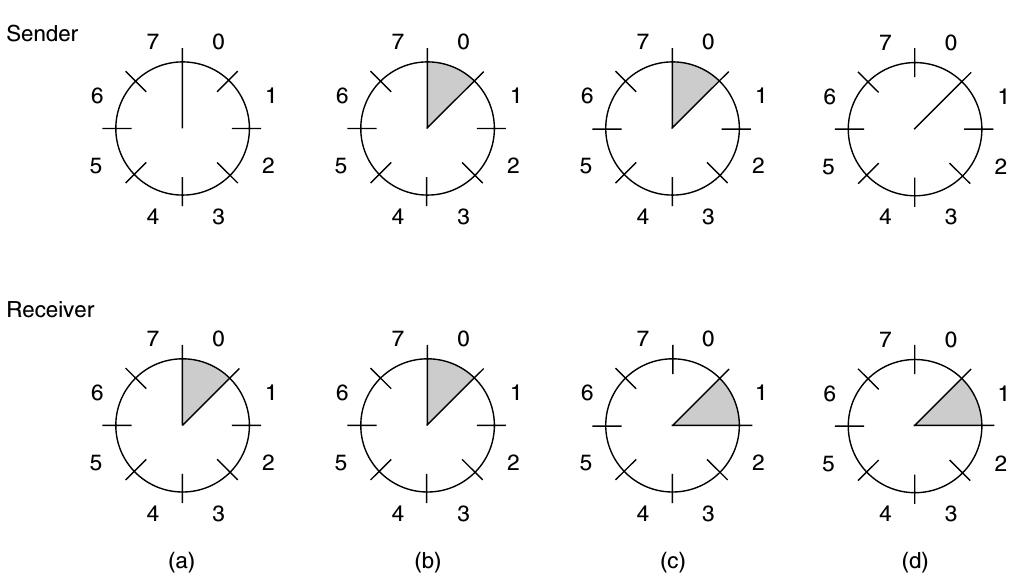
\includegraphics[scale=0.6]{Images/slidingwindow1}
\label{fig:cn_sliding_window_1}
\end{figure}
\subsubsection{1 bit Sliding Window Protocol}
Assume that computer A is trying to send its frame 0 to computer B and that B is trying to send its frame 0 to A. Suppose that A sends a frame to B, but A's timeout interval is a little too short. Consequently, A may time out repeatedly, sending a series of identical frames, all with seq = 0 and ack = 1. When the first valid frame arrives at computer B, it will be accepted and frame expected will be set to a value of 1. All the subsequent frames received will be rejected because B is now expecting frames with sequence number 1, not
0. Furthermore, since all the duplicates will have ack = 1 and B is still waiting for an acknowledgement of 0, B will not go and fetch a new packet from its network layer.\\
After every rejected duplicate comes in, B will send A a frame containing seq = 0 and ack = 0. Eventually, one of these will arrive correctly at A, causing A to begin sending the next packet. No combination of lost frames or premature timeouts can cause the protocol to deliver duplicate packets to either network layer, to skip a packet, or to deadlock. The protocol is correct.
\begin{figure}[H]
\caption{ (a) Normal case. (b) Abnormal case. The notation is (seq, ack, packet number). An asterisk indicates where a network layer accepts a packet.}
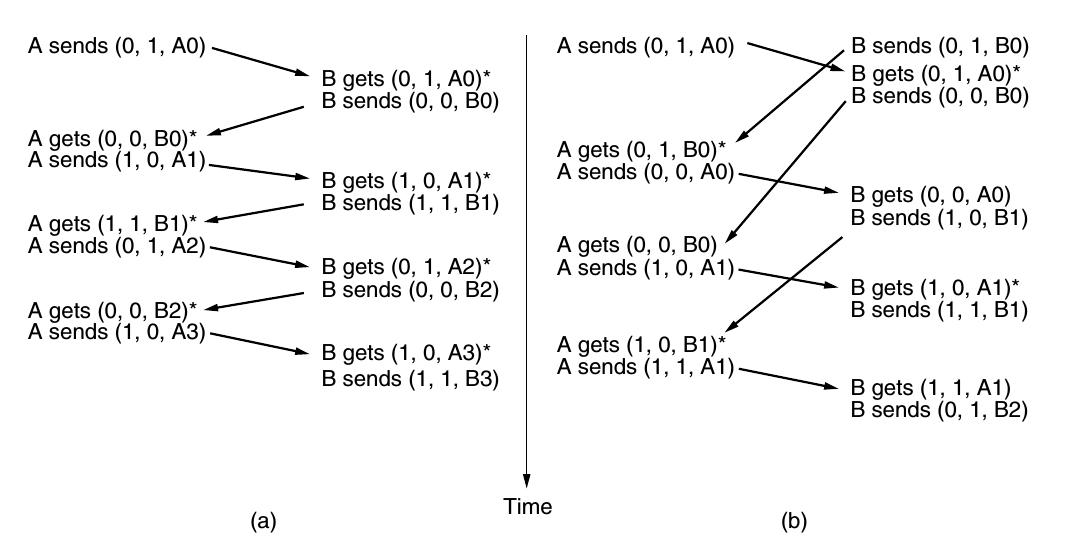
\includegraphics[scale=0.6]{Images/slidingwindow2}
\label{fig:cn_1bit_slide}
\end{figure}
\subsubsection{Go Back N}
$\text{Bandwidth Delay Product(BDP)} = \text{Bandwidth(bits/sec)} \times \text{One-way transit time}$\\
$BD = \dfrac{BDP}{\text{No. of frames}}$\\
Max no. of frames to be sent before blocking = Max. window size = $w = 2BD + 1$.
$$ \text{Link Utilization} \le \dfrac{w}{2BD + 1}$$
\begin{figure}[H]
\caption{Pipelining and error recovery. Effect of an error when (a) receiver's window size is 1(Go Back n) and (b) receiver's window size is large(Selective Repeat).}
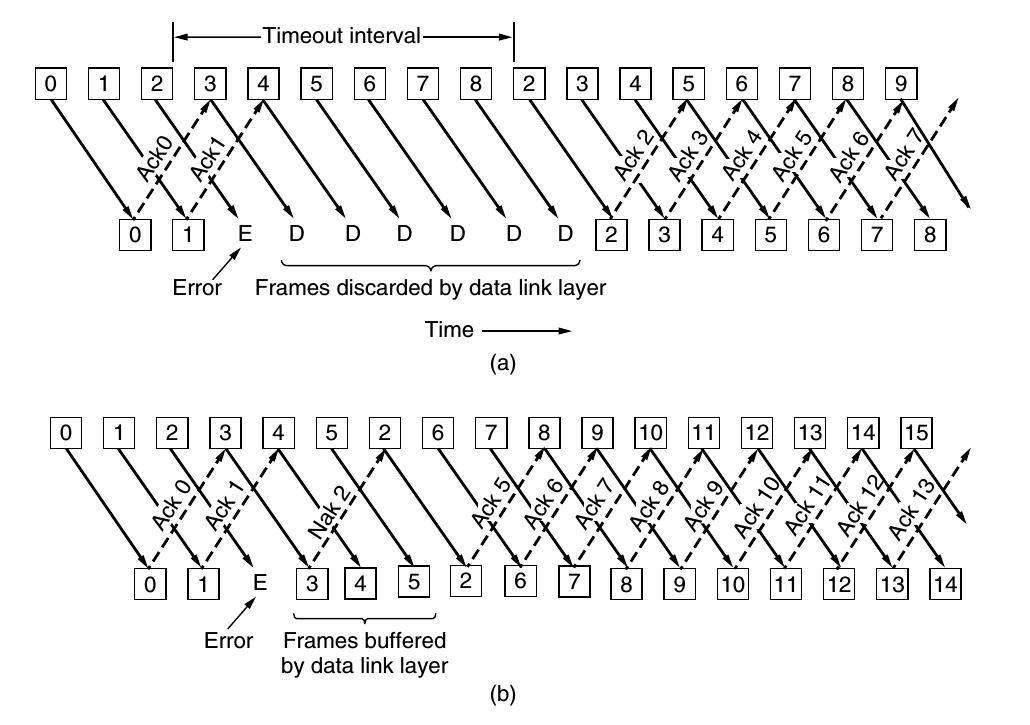
\includegraphics[scale=0.6]{Images/gobacknselectiverepeat}
\label{fig:cn_select_repeat}
\end{figure}
\subsubsection{Selective Repeat}
\todo{Please understand seletive repeat}
\begin{figure}[H]
\caption{(a) Initial situation with a window of size 7. (b) After 7 frames have been sent and received but not acknowledged. (c) Initial situation with a window size of 4. (d) After 4 frames have been sent and received but not acknowledged.}
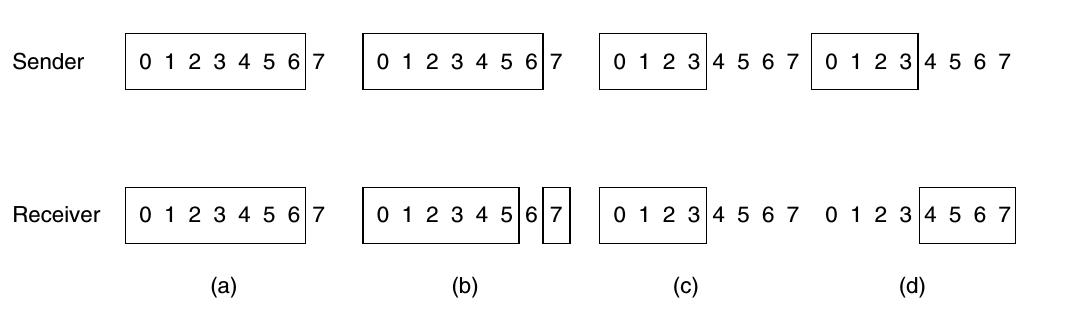
\includegraphics[scale=0.6]{Images/selectiverepeat}
\label{fig:cn_selective_repeat}
\end{figure}
Window size $\le$ Sequence number. \cite{selectiverepeat1}, \cite{selectiverepeat}, \cite{srgobackn}.
What is the maximum window size? The receiver must be able to distinguish a retransmission of an already received packet from the original transmission of a new packet. Thus the maximum window size is:
\begin{enumerate}
\item $2^n - 1$ in the case of Go-Back-N. Here the receiver accepts only the next expected packet and discards all out-of-order packets. In the example, with a 2-bit sequence number the maximum window size is 3
\item $\dfrac{2^n}{2}$ in Selective Repeat. Since the receiver accepts out-of-order packets, two consecutive windows should not overlap. Otherwise it is not able to distinguish duplicates from new transmissions. Hence, in the example the maximum window size is 2
\end{enumerate}
\chapter{Data Link Layer Switching}
\section{Bridges}
\begin{definition}[Bridges]
Bridges are used for connecting multiple LAN's  into a single logical LAN in an organization. Bridges operate in the data link layer, so they examine the data link layer addresses to forward frames. They can handle IP packets as well as other kinds of packets. Different kinds of cables can also be attached to one bridge. 
\end{definition}
\begin{definition}[VLAN(Virtual LAN)]
Treat one physical LAN as multiple logical LANs.
\end{definition}
\begin{figure}[H]
\caption{a) Bridge connecting two multidrop LANs. (b) Bridges (and a hub) connecting seven point-to-point stations.}
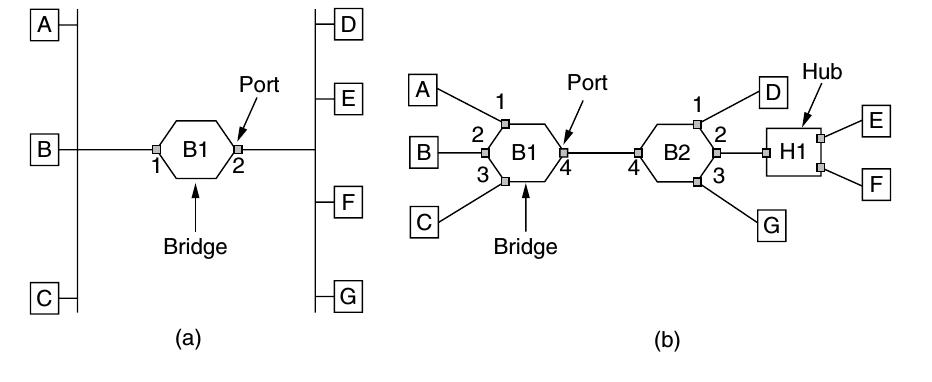
\includegraphics[scale=0.6]{Images/bridges}
\label{fig:cn_bridges}
\end{figure}
\subsection{Learning Bridges}
The bridge must decide whether to forward or discard each frame, and, if the former, on which port to output the frame. A simple way to implement this scheme is to have a big (hash) table inside the bridge. The table can list each possible destination and which output port it belongs on. \\
When the bridges are first plugged in, all the hash tables are empty. None of the bridges know where any of the destinations are, so they use a flooding algorithm: every incoming frame for an unknown destination is output on all the ports to which the bridge is connected except the one it arrived on. As time goes on, the bridges learn where destinations are. Once a destination is known, frames
destined for it are put only on the proper port; they are not flooded.\\
To handle dynamic topologies, whenever a hash table entry is made, the arrival time of the frame is noted in the entry. Whenever a frame whose source is already in the table arrives, its entry is updated with the current time. Thus, the time associated with every entry tells the last time a frame from that machine was seen.\\
The routing procedure for an incoming frame depends on the port it arrives on (the source port) and the address to which it is destined (the destination address).
\begin{enumerate}
\item If the port for the destination address is the same as the source port, discard the frame.
\item If the port for the destination address and the source port are different, forward the frame on to the destination port.
\item If the destination port is unknown, use flooding and send the frame on all ports except the source port.
\end{enumerate}
Bridges only look at the MAC addresses to decide how to forward frames, it is possible to start forwarding as soon as the destination header field has come in, before the rest of the frame has arrived (provided the output line is available, of course). This design reduces the latency of passing through the bridge, as well as the number of frames that the bridge must be able to buffer. It is referred to as \textbf{cut-through switching or wormhole routing} and is usually handled in hardware.
\subsection{Spanning Trees}
\begin{figure}[H]
\caption{Bridges with two parallel links.}
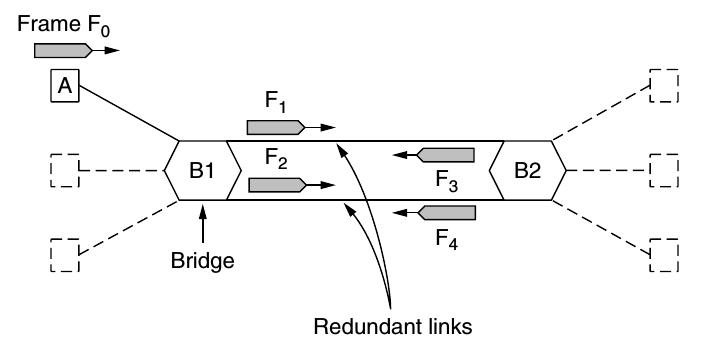
\includegraphics[scale=0.6]{Images/spanningTreecn}
\label{fig:cn_spanning_tree}
\end{figure}
Bridges to communicate with each other and overlay the actual topology with a spanning tree that reaches every bridge (to avoid looping). \\
To build the spanning tree, the bridges run a distributed algorithm. Each bridge periodically broadcasts a configuration message out all of its ports to its neighbors and processes the messages it receives from other bridges, as described next. These messages are not forwarded, since their purpose is to build the tree, which can then be used for forwarding.\\
To make the choice of root, they each include an identifier based on their MAC address in the configuration message, as well as the identifier of the bridge they believe to be the root. MAC addresses are installed by the manufacturer and guaranteed to be unique worldwide, which makes these identifiers convenient and unique. The bridges choose the bridge with the lowest identifier to be the root.\\
To find these shortest paths, bridges include the distance from the root in their configuration messages. Each bridge remembers the shortest path it finds to the root. The bridges then turn off ports that are not part of the shortest path.
\begin{figure}[H]
\caption{ (a) Which device is in which layer. (b) Frames, packets, and headers.}
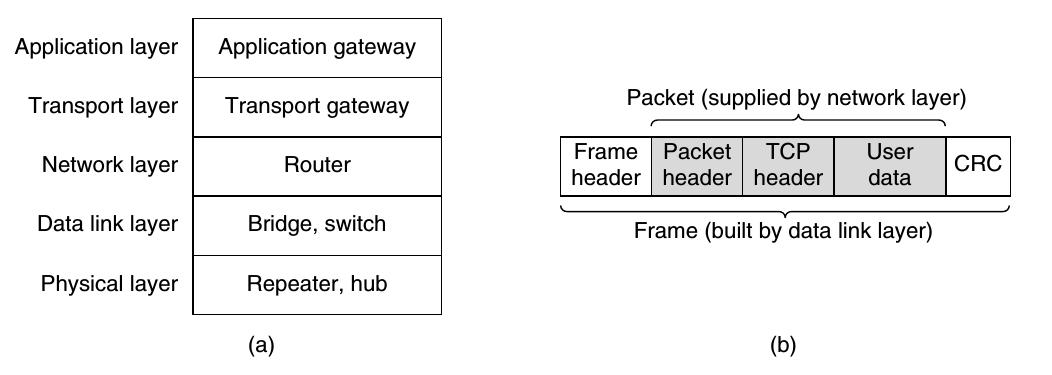
\includegraphics[scale=0.6]{Images/sample}
\label{fig:cn_layer}
\end{figure}
\chapter{Transport Layer}
\section{Introduction}
\begin{figure}[H]
\caption{The primitives of Transport Layer.}
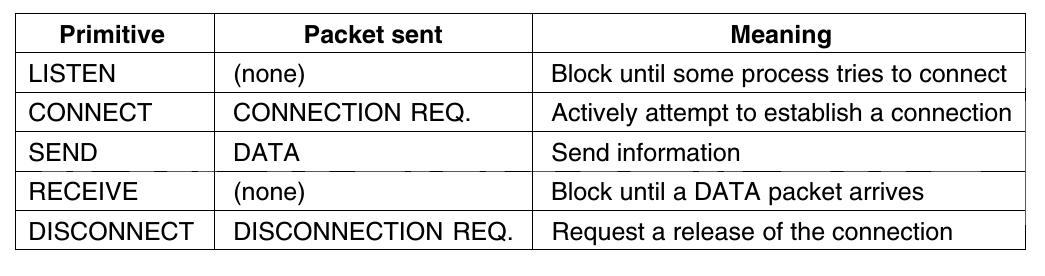
\includegraphics[scale=0.6]{Images/primitivestransport}
\label{fig:cn_primitives_transport_layer}
\end{figure}
\begin{figure}[H]
\caption{The primitives of TCP socket.}
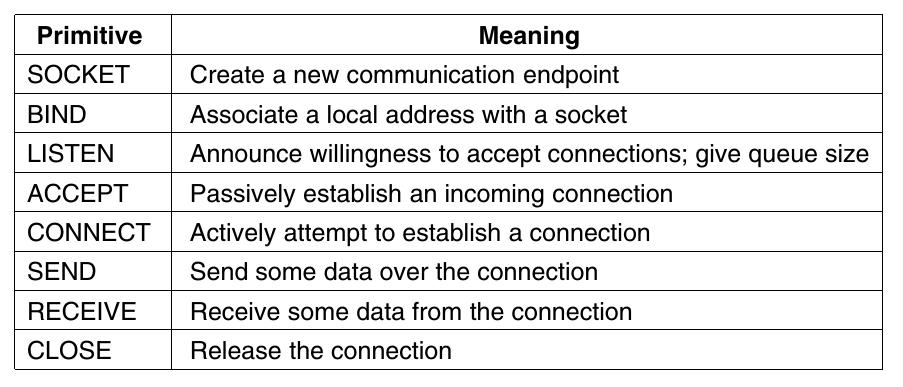
\includegraphics[scale=0.6]{Images/tcpsocketprim}
\label{fig:cn_tcp_primitives}
\end{figure}
\chapter{Internet Protocol - IP}
\section{IPv4}
\begin{figure}[H]
\caption{IPv4 Header}
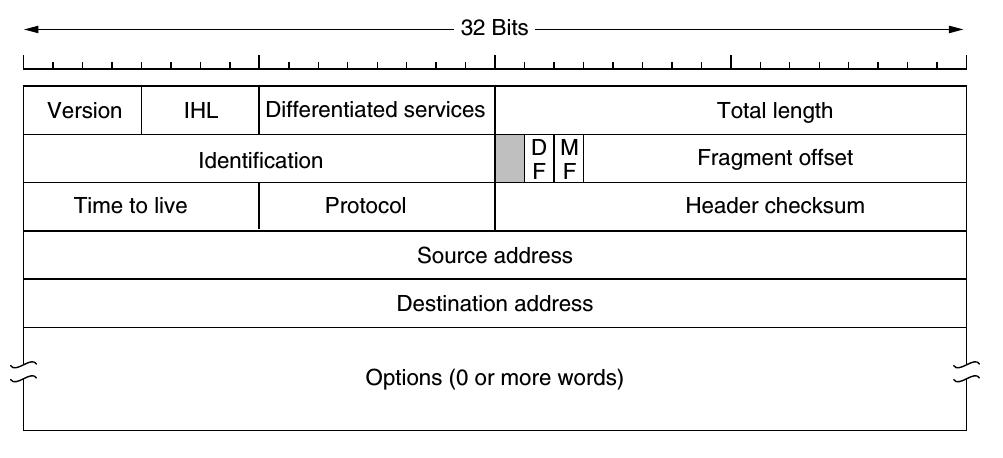
\includegraphics[scale=0.6]{Images/ipv4header}
\label{fig:cn_ipv4_head}
\end{figure}
\chapter{Network Layer}
\begin{enumerate}
\item Physical Address - MAC Address: System Address:LAN card address:Ethernet address. Points to main memory.
\item Communication done with logical address - IP address. Types: Classful addressing, subnetting, supernetting.
\begin{enumerate}
\item Classful Addressing: 2 parts: net-id, hosts; 2 notations: binary: 00000011 00000011 00000011 00000011, octet: 255.255.255.255
\item Unicasting: Transfer data from one system to another system. Supported by class A,B,C.
\item Multicasting: Transfers data from one systems to many systems. Suported by Class D.
\item Class E : Future Use. First 4 bits in net-ID: 1111. IP address range(240 - 255). 
\end{enumerate}
\end{enumerate}
\begin{enumerate}
\item \textbf{Part of CIDR (Classless Inerdomain Routing)}
\item Class A: $1^{st}$ bit of net ID should be 0. net-ID(8 bits): $2^7 - 2$ bits(no. of possible networks). host-ID(24 bits): $2^{24} - 2$(no. of possible hosts). IP address range(0 -126). 0.0.0.0 - DHCP, 127.x.y.z - Loopback.
\item Class B: $1^{st}, 2^{nd}$ bit of net ID should be 10. net-ID(16 bits): $2^{14}$ bits(no. of possible networks). host-ID(16 bits): $2^{16} - 2$(no. of possible hosts). IP address range(128 -191). 
\item Class C: $1^{st}, 2^{nd}, 3^{rd}$ bit of net ID should be 110. net-ID(24 bits): $2^{21}$ bits(no. of possible networks). host-ID(8 bits): $2^{8} - 2$(no. of possible hosts). IP address range(192 -223). 
\item Class D: $1^{st}, 2^{nd}, 3^{rd}, 4^{th}$ bit of net ID should be 1110. net-ID( bits): $2^{}$ bits(no. of possible networks). host-ID( bits): $2^{} - 2$(no. of possible hosts). IP address range(224 - 239). 
\item Class D \& Class E cannot be divided into net-ID \& host-ID because of multicasting.
\item Net masks for various classes:(net-ID all 0's and host-Id all 1's) \todo{Check about net mask}
\begin{enumerate}
\item Class A - 255.0.0.0
\item Class B - 255.255.0.0
\item Class C - 255.255.255.0
\end{enumerate}
\item Calculation of net-ID:
\begin{enumerate}
\item Identify class of IP address. 
\item Calculate net mask for that class.
\item Perform bitwise AND operation between IP address and net mask.
\end{enumerate}
\item Range of private IP addresses:(for communication within LAN)
\begin{enumerate}
\item Class A: 10.0.0.0 - 10.255.255.255 - 1n/w
\item Class B: 172.16.0.0 - 172.31.255.255 - 16 n/w
\item Class C: 192.168.0.0 - 192.168.255.255 - 255 n/w
\end{enumerate}
\item NAT -  Network Address Translator. Converts private IP to public IP when pkt going outside the n/w \& public IP to private IP if pkt coming in the n/w.
\item Destination Broadcast address
\item Limited Broadcast address
\end{enumerate}
\begin{enumerate}
\item Service addressing system - Port address: 16 bits. also known as logical ports
\item Predefined ports like http, smtp etc., (0 - 1023).
\item Registered ports (1024 - 49151)
\item Dynamic Ports - (49152 - 65535)
\item \todo{Learn about \textbf{DHCP}}
\end{enumerate}
\section{Subnetting}
\begin{enumerate}
\item Borrows bits from host-ID. Security is high.
\item Given subnet mask, we can calculate no. of subnets and  no. of hosts in each subnet
\item Subnet-ID = IP Address AND subnet mask.
\item \textbf{Example}: Subnet mask of class B: 255.255.240.0. Default Mask for class B: 255.255.0.0. Subnet bits are no. of bits having 1's in the host bits of mask. \\
Subnet mask = $\underbrace{255.255}_\text{Net-ID}.\underbrace{240}_\text{subnet}.\underbrace{0}_\text{host}$\\
No. of subnets = $2^4 - 2 = 14$. no. of hosts in each subnet = $2^{12} - 2 = 4094$
\item \textbf{Example}: IP address: 197.111.121.199 \& Subnet mask: 255.255.255.240. Calculate subnet-ID.\\
197.111.121.199 \& 255.255.255.240 = 197.111.121.192\\
197.111.121.192 = 11000101.01101111.01111001.11000000. no. of 1's in host part = 4. Total no .of subnets = 14. Total no. of hosts = 126.
\begin{enumerate}
\item /28 means 28 1's in the subnet mask.
\item $1^{st}$ subnet id: 197.111.121.16/28(in slash notaion of CIDR) - 11000101.01101111.01111001.00010000
\item $2^{nd}$ subnet id: 197.111.121.32/28 - 11000101.01101111.01111001.00100000
\item $3^{rd}$ subnet id: 197.111.121.48/28 - 11000101.01101111.01111001.00110000
\item Last subnet id: 197.111.121.224/28 - 11000101.01101111.01111001.11100000
\item Last host of subnet id: 197.111.121.238/28 - 11000101.01101111.01111001.11101110
\end{enumerate}
\end{enumerate}
\section{Classless Addressing}
\begin{enumerate}
\item It consists of only blocks.
\item IP address given along with mask.
\item $1^{st}$ address of the block should be divisible by no. of addresses in the block.
\item Addresses must be contiguous.
\item Every address in a block must be a power of 2.
\item \textbf{Example}: One of the addresses in a block is 167.199.170.82/27. find no. of addresses and $1^{st}$ \& last address.\\
This block consists of No .of hosts = $2^5 = 32$. No. of address in a block is determined by subnet mask.\\
$1^{st}$ address $82 \to 01010010$. Replace the last 5 bits by 0's. Therefore $1^{st}$ address is 01000000. Last address is 01011111.
\item When all subnet bits are 0 $\to$ zero subnet.
\item When all subnet bits are 1 $\to$ all ones subnet.
\end{enumerate}
\chapter{Physical Layer}
\section{Introduction}
\begin{definition}[Transmission time]
Time taken to place the data on the channel.
$$ \text{Transmission Time}(T_X) = \dfrac{\text{Mesage size}}{\text{Bandwidth}}$$
$$ \text{Transmission Time}(T_{ack}) = \dfrac{\text{Acknowledgement size}}{\text{Bandwidth}}$$
\end{definition}
\begin{definition}[Propagation Time]
Time taken by data to propagate to reach the destination.
$$ \text{Propagation Time}(P_X) = \dfrac{\text{Distance}}{\text{Velocity}} $$
$$ \text{Propagation Time}(P_{ack}) = \dfrac{\text{Distance}}{\text{Velocity}} $$\\
\end{definition}
$$ \text{Total Time} = T_{X} + P_X + P{ack} = T_X + 2P_X$$
$$ \text{Link Utilization of Sender} = \dfrac{T_X}{\text{Total Time}} = \dfrac{\text{Message size}}{\text{Message size + Bandwidth*RTT}}$$
$$ \text{Round Trip Time(RTT)} = 2 \times P_X $$
\begin{definition}[Processing Time]
Time taken to generate the data.
\end{definition}
\begin{enumerate}
\item At sender headers are added \& at receiver headers are removed.
\item Physical address points to Data Link Layer - Bridge
\item Logical address points to Network Layer - Router
\item Port address points to Transport Layer - Gateway
\end{enumerate}




















\part{Calculus}
\chapter{Continuity}
\begin{definition}[Continuity]
\label{Continuity}
Let $D \in \mathbb{R}$ . Consider a function $f : D \rightarrow
\mathbb{R}$ and a point $c \in D$. We say that $f$ is \textbf{continuous} at
$c$ if 
\begin{center}
($x_n$) any
sequence in $D$ and $x_n \rightarrow c \implies f(x_n) \rightarrow f(c)$.
\end{center}
If $f$ is not continuous at $c$, we say that $f$ is \textbf{discontinuous} at
$c$. In case $f$ is continuous at every $c \in D$, we say that $f$ is continuous
on $D.$
\end{definition}
\begin{definition}[Dirichlet Function]
$$ f(x) = \left\{ 
  \begin{array}{l l}
    1 & \quad \text{if $x$ is rational}\\
    0 & \quad \text{if $x$ is irrational}
  \end{array} \right.$$
  \label{Dirichlet Function}
\end{definition}
\begin{lemma}
Let D $\subseteq \mathbb{R}, c \in D$, and let $f : D \rightarrow \mathbb{R}$ be a function that is
continuous at $c$. If $f(c) > 0$, then there is $\delta > 0$ such that $f(x) > 0$ whenever
$x \in D$ and $\left|x - c\right| < \delta$. Likewise, if $f(c) < 0$, then there is $\delta > 0$ such that
$f(x) < 0$ whenever $x \in D$ and $\left|x - c\right| < \delta$.
\end{lemma}
\begin{proposition}
Let $D \subseteq R, c \in D$, and let $f, g : D \to R$ be functions that
are continuous at $c$. Then
\begin{enumerate}
\item $f + g$ is continuous at $c$,
\item $rf$ is continuous at $c$ for any $r \in R$,
\item $fg$ is continuous at $c$,
\item if $ f(c) = 0$, then there is $ \delta > 0$ such that $f (x) = 0$ whenever $x \in D$ and $\left|x-c\right| < \delta$; moreover the function $ \dfrac{1}{f} : D \cap (c- \delta, c+ \delta) \to R$ is continuous
at $c$, 
\item if there is $ \delta > 0$ such that $f (x) \ge 0$ whenever $x \in D$ and $\left|x-c\right| < \delta $, then for any $k \in N$, the function $f^{\dfrac{1}{k}} : D \cap (c - \delta, c + \delta) \to R$ is continuous at $c$.
\end{enumerate}
\end{proposition}
\chapter{Differentiation}
\begin{lemma}
Let $D \subseteq R$ and $c$ be an interior point of $D$. If $f : D \to R$ is
differentiable at $c$ and has a local extremum at $c$, then $f (c) = 0$.
\end{lemma}
\begin{proposition}[Rolle's Theorem]
If $f : \left[a,b\right] \to R$ is continuous on $\left[a,b\right]$ and differentiable on $(a, b)$ and if $f (a) = f (b)$, then there is $c \in (a, b)$
such that $f (c) = 0$.
\end{proposition}
\begin{proposition}[Mean Value Theorem]
If a function $f : \left[a,b\right] \to R$ is continuous on $\left[a,b\right]$ and differentiable on $(a, b)$, then there is $c \in (a, b)$ such that
$$f (b) - f (a) = f'(c)(b - a).$$
\end{proposition}
\chapter{Integration}
\begin{proposition}
Let $f : \left[a,b\right] \to R$ be a bounded function. Then for any
partition $P$ of $\left[a,b\right]$, we have 
 $$ m(f )(b - a) \le L(P, f ) \le U (P, f ) \le M (f )(b - a). $$
 where 
 $$  L(P, f ) :=  \sum_{i=0}^{n} m_i (f )(x_i - x_{i-1} )$$
 $$  U (P, f ) :=  \sum_{i=0}^{n} M_i (f )(x_i - x_{i-1} ).$$
 L(P, f) = Lower Sum, U(P, f) = Upper Sum
\end{proposition}
\begin{proposition}[Basic Inequality on Riemann's Integral]
 Suppose $f : \left[a,b\right]  \to R$ is an integrable function and there are $\alpha, \beta \in R$ such that $ \beta \le f \le \alpha$. Then
$$ \beta (b - a) \le \int_{a}^{b} f (x)dx \le \alpha(b - a). $$. In particular, if $\left|f\right| \le \alpha$, then
$$ \int_{a}^{b} f (x)dx \le \alpha(b - a). $$
\end{proposition}
\begin{proposition}[Domain Additivity of Riemann Integrals]
 Let $f : [a, b] \to R$ be a bounded function and let $c \in (a, b)$. Then f is integrable on $\left[a,b\right]$ if and only if f is integrable on $\left[a,c\right]$ and on $\left[c,b\right]$. In this case,
$$ \int_{a}^{b} f(x)dx = \int_{a}^{c} f(x)dx + \int_{c}^{b} f(x)dx$$
\end{proposition}
\begin{proposition}
 Let $f : [a, b] \to R$ be a function.
\begin{enumerate}
\item If f is monotonic, then it is integrable.
\item If f is continuous, then it is integrable.
\end{enumerate}
\end{proposition}
\begin{proposition}
Let $f, g : [a, b] \to R$ be integrable functions. Then
\begin{enumerate}
\item $f + g$ is integrable and $\int_{a}^{b}(f + g)(x)dx = \int_{a}^{b}f (x)dx + \int_{a}^{b}g(x)dx$,
\item $rf$ is integrable for any r ∈ R and a b
 $ \int_{a}^{b}(rf )(x)dx = r \int_{a}^{b} f (x)dx$,
\item $fg$ is integrable,
\item If there is $ \delta > 0$ such that $\left|f(x)\right| \ge \delta$ and all $x \in [a, b]$, then $\dfrac{1}{f}$ is integrable,
\item If $f (x) \ge 0$ for all $x \in [a, b]$, then for any $k \in N$, the function $f^{\dfrac{1}{k}}$ is integrable.
\end{enumerate}
\end{proposition}
\begin{proposition}
Let $f, g : [a, b] \to R$ be integrable.
\begin{enumerate}
\item If $f \le g$, then  $\int_{a}^{b} f (x)dx \le \int_{a}^{b} g(x)dx$.
\item The function $\left|f\right|$ is integrable and $ \left|\int_{a}^{b} f (x)dx\right| \le  \int_{a}^{b} \left|f\right|(x)dx$.
\end{enumerate}
\end{proposition}
\begin{proposition}[Fundamental Theorem of Calculus]
 Let $f : [a, b] \to R$ be integrable.
 \begin{enumerate}
\item If $f$ has an antiderivative $F$ , then
$$ \int_{a}^{x}f (t)dt = F (x) - F (a)  \text{ for all } x \in [a, b]$$.
\item Let $F : [a, b] \to R$ be defined by
$$F (x) = \int_{a}^{x} f (t)dt.$$
If $f$ is continuous at $c \in [a, b]$, then $F$ is differentiable at $c$ and
$$ F'(c) = f (c). $$ In particular, if $f$ is continuous on $[a, b]$, then $F$ is an antiderivative of $f$
on $[a, b]$.
 \end{enumerate}
\end{proposition}
\begin{proposition}[Fundamental Theorem of Riemann Integration]
Let $F : [a, b] \to R$ be a function. Then $F$ is differentiable
and $F'$ is continuous on $[a, b]$ if and only if there is a continuous function $f : [a, b] \to R$ such that
 $$F (x) = F (a) + \int_{a}^{x}f (t)dt \text{ for all } x \in [a, b].$$
In this case, we have $F'(x) = f (x)$ for all $x \in [a, b]$.
\end{proposition}
\chapter{Definite Integrals \& Improper Integrals}



















\part{Linear Algebra}
\chapter{Determinants}
\section{Introduction}
\section{Properties}
\begin{enumerate}
\item $\left|A^{\text{t}}\right| = \left|A\right|$
\item$\left|A\right| = 0$ if:
\begin{enumerate}
\item It has two equal lines.
\item All elements of a line are zero.
\item The elements of a line are a linear combination of the others.
\end{enumerate}
\item A triangular determinant is the product of the diagonal elements.
\item If a determinant switches two parallel lines its determinant changes sign.
\item If the elements of a line are added to the elements of another parallel line previously multiplied by a real number, the value of the determinant is unchanged.
\item If a determinant is multiplied by a real number, any line can be multiplied by the above mentioned number, but only one.
\item  If all the elements of a line or column are formed by two addends, the above mentioned determinant decomposes in the sum of two determinants.
\item $\left|A.B\right| = \left|A\right|.\left|B\right|$.
\item If $A$ is invertible, then $\left|A^{-1}\right| = \dfrac{1}{\left|A\right|}$.
\item Suppose if 2 rows of a square matrix "A" are the same, then $\left|A\right| = 0$.
\item $\left|cA\right| = c^n\left|A\right|$ for an $n \times n$ matrix.
\item $A^{-1} = \dfrac{\text{adj(A)}}{\left|A\right|}$.
\item Vandermode determinant:
$\left|
\begin{array}{ccccc}
 1 & 1 & 1 & \cdots  & 1 \\
 x_1 & x_2 & x_3 & \cdots  & x_n \\
 x_1^2 & x_2^2 & x_3^2 & \cdots  & x_n^2 \\
 \vdots  & \vdots  & \vdots  & \ddots & \vdots  \\
 x_1^{n-1} & x_2^{n-1} & x_3^{n-1} & \cdots  & x_n^{n-1}
\end{array}
\right|=\prod _{1\leq i<j\leq n} \left(x_j-x_i\right)$
\item Circulant Matrix:
$\left|
\begin{array}{ccccc}
 x_1 & x_2 & x_3 & \cdots  & x_n \\
 x_n & x_1 & x_2 & \cdots  & x_{n-1} \\
 x_{n-1} & x_n & x_1 & \cdots  & x_{n-2} \\
 \vdots  & \vdots  & \vdots  & \ddots & \vdots  \\
 x_2 & x_3 & x_4 & \cdots  & x_1
\end{array}
\right|=\prod _{j=1}^n \left(x_1+x_2\omega _j+x_3\omega _j^2+\ldots +x_n\omega _j^{n-1}\right)$
where $\omega_j$ is an $n^{\text{th}}$ root of 1.
\item $\left|A\right| = \left|A^T\right| = \left|-A\right| = (−1)^n\left|A\right|$. Hence $det(A) = 0$ when $n$ is odd.
\end{enumerate}
\section{Determinants \& Eigenvalues}
\begin{enumerate}
\item $\left|A - xI\right| = 0$.
\item A symmetric $n \times n$ real matrix $M$ is said to be \textbf{positive definite} if $z^TMz$ is positive for every non-zero column vector $z$ of $n$ real numbers. Here $z^T$ denotes the transpose of $z$.
\item The negative definite, positive semi-definite, and negative semi-definite matrices are defined in the same way, except that the expression $z^TMz$ or $z*Mz$ is required to be always negative, non-negative, and non-positive, respectively.
\item Eigenvalues of Hermitian Matrices( $A = \overline {A^\text{T}}$ ) are always real.
\item For any real non-singular matrix $A$, the product  $A^T A$  is a \textbf{positive definite} matrix. 
\item All eigenvalues of positive definite matrix are positive.
\item Every positive definite matrix is invertible and its inverse is also positive definite.
\item If $M$ is positive definite and $r > 0$ is a real number, then $rM$ is positive definite. If $M$ and $N$ are positive definite, then the sum $M + N$ and the products $MNM$ and $NMN$ are also positive definite. If $MN = NM$, then $MN$ is also positive definite.($M \& N$ are square matrices.)
\item Every principal submatrix of a positive definite matrix is positive definite.
\item The trace tr(A) is by definition the sum of the diagonal entries of A and also equals the sum of the eigenvalues.
\item $\mathrm{tr}(A) = \log(\left|(\exp(A))\right|)$.,
\end{enumerate}
\section{Eigenvectors \& Eigenvalues}
\begin{enumerate}
\item Eigenvectors with Distinct Eigenvalues are Linearly Independent.
\item Singular Matrices have Zero Eigenvalues. ie, eigenvalue = 0.
\item Suppose $A$ is a square matrix and $\lambda$ is an eigenvalue of $A$. Then $\alpha \lambda$ is an eigenvalue of $\alpha A$.
\item Suppose $A$ is a square matrix, $\lambda$ is an eigenvalue of $A$, and $s \ge 0$ is an integer. Then $\lambda^s$ is an eigenvalue of $A^s$.
\item Suppose A is a square matrix and $\lambda$ is an eigenvalue of A. Let q(x) be a polynomial in the variable x. Then q($\lambda$) is an eigenvalue of the matrix q(A).
\item Suppose A is a square nonsingular matrix and $\lambda$ is an eigenvalue of A. Then $\lambda^{-1}$ is an eigenvalue of the matrix $A^{-1}$.
\item Suppose A is a square matrix and $\lambda$ is an eigenvalue of A. Then $\lambda$ is an eigenvalue of the matrix $A^t$.
\item Suppose A is a square matrix with real entries and x is an eigenvector of A for the eigenvalue $\lambda$. Then $\bar{x}$ is an eigenvector of A for the eigenvalue $\bar{\lambda}$.
\item Hermitian Matrices have Real Eigenvalues, orthogonal eigenvectors.
\item An eigenvalue $\lambda$ has algebraic multiplicity $l > 0$ if $\det(A - \lambda I) = 0$.
\item Characteristic Polynomial: $\det(A - \lambda I) = 0$.
\item An $n \times n$ symmetric matrix has $n$ orthogonal eigenvectors( $X^TY = 0$) for distinct eigenvalues.
\item Symmetric matrices only have real eigenvalues.
\item \textbf{Geometric multiplicity} $\gamma_T(\lambda)$ of an eigenvalue $\lambda$ is the dimension of the eigenspace associated to $\lambda$, i.e. number of linearly independent eigenvectors with that eigenvalue.
\item Let A be an arbitrary $n \times n$ matrix of complex numbers with eigenvalues $\lambda_1, \lambda_2, ... \lambda_n$. 
\begin{enumerate}
\item Every eigenvalue of a unitary matrix has absolute value $|\lambda| = 1$.
\item If $A$ is invertible, then the eigenvalues of $A^{-1}$ are $1/\lambda_1,1/\lambda_2,\dots,1/\lambda_n$.
\item The eigenvalues of the $k^{\text{th}}$ power of A, i.e. the eigenvalues of $A^k$, for any positive integer $k$, are $\lambda_1^k,\lambda_2^k,\dots,\lambda_n^k$ with same eigenvectors.
\item The matrix A is invertible if and only if all the eigenvalues $\lambda_i$ are nonzero.
\item The trace of A, defined as the sum of its diagonal elements, is also the sum of all eigenvalues:
$\operatorname{tr}(A) = \sum_{i=1}^n A_{i i} = \sum_{i=1}^n \lambda_i = \lambda_1+ \lambda_2 +\cdots+ \lambda_n$.
\item The determinant of A is the product of all eigenvalues:
$\operatorname{det}(A) = \prod_{i=1}^n \lambda_i=\lambda_1\lambda_2\cdots\lambda_n$.
\item New Item
\end{enumerate}
\item The eigenvalues of a diagonal or triangular matrix are its diagonal elements.
\item An $n \times n$ matrix is invertible if and only if it doesn't have 0 as an eigenvalue.
\item Row reductions don't preserve eigenvalues . However, similar matrices have the same characteristic polynomial, so theyhave the same eigenvalues with the same multiplicities.
\item A complete set of eigenvectors for $A_{n \times n}$ is any set of $n$ linearly independent eigenvectors for $A$.
\item A $n \times n$ is diagonalizable if and only if $A$ possesses a complete set ofeigenvectors. Moreover,$P^{−1}AP = diag(\lambda_1, \lambda_2, \ldots, \lambda_n)$ if and only if the columns of $P$ constitute a complete set of eigenvectors and the $\lambda_j$'s are the associated eigenvalues.
\item \textbf{Cayley Hamilton Theorem}: Every square matrix satisfiesits own characteristic equation $p(\lambda) = 0$.That is, $p(A) = 0$.
\item If no eigenvalue of A is repeated, then A is diagonalizable. Converse is not true.
\end{enumerate}
\section{Cramer's rule}
A linear system of $m$ equations with $n$ unknowns $x_1, x_2, \ldots, x_n$.
\begin{alignat*}{9}
a_{11}x_1 & {}+{} &  a_{12}x_2 & {}+{} & \ldots & {}+{} & a_{1n}x_n & {}={} & b_1 \\
a_{21}x_1 & {}+{} &  a_{22}x_2 & {}+{} & \ldots & {}+{} & a_{2n}x_n & {}={} &  b_2 \\
\vdots    & {}+{} &  \vdots    & {}+{} & \vdots & {}+{} & \vdots    & {}={} &  \vdots \\
a_{m1}x_1 & {}+{} &  a_{m2}x_2 & {}+{} & \ldots & {}+{} & a_{mn}x_n & {}={} & b_m \\
\end{alignat*}
\textbf{Solution}:\\
$x_1$ = $\dfrac{A_1}{A}$, $\ldots$ $x_i$ = $\dfrac{A_i}{A}$ $\ldots$, $x_n$ = $\dfrac{A_n}{A}$ where 
$$ A_i = \begin{vmatrix}
a_{11} & a_{12} & \ldots & b_1 & \ldots & a_{1n} \\
a_{21} & a_{22} & \ldots & b_2 & \ldots & a_{2n} \\
\vdots & \vdots & \ldots & \vdots & \ldots & \vdots \\
a_{m1} & a_{m2} & \ldots & b_n & \ldots & a_{mn}
\end{vmatrix}$$
where $b_i$'s are present in $i^{\text{th}}$ column.
\section{Rank of a Matrix}
\begin{enumerate}
\item The rank of a matrix is the number of pivots when in row echelon form. A pivot is the first non zero entry in a row.
\item Rank of diagonal matrix is the no. of non-zero elements in the principal diagonal of the matrix.
\item Rank of $A$ ($m \times n$) matrix is $\text{rank}(A) \le (m, n)$.
\item A square matrix $A$ of order $n$ is invertible if rank(A) = n.
\item Rank(A) + nullity(A) = no. of columns in A.
\item Row equivalent matrices have same rank.
\end{enumerate}
\section{System of Linear Equations}
A linear system of $m$ equations with $n$ unknowns $x_1, x_2, \ldots, x_n$.
\begin{alignat*}{9}
a_{11}x_1 & {}+{} &  a_{12}x_2 & {}+{} & \ldots & {}+{} & a_{1n}x_n & {}={} & b_1 \\
a_{21}x_1 & {}+{} &  a_{22}x_2 & {}+{} & \ldots & {}+{} & a_{2n}x_n & {}={} &  b_2 \\
\vdots    & {}+{} &  \vdots    & {}+{} & \vdots & {}+{} & \vdots    & {}={} &  \vdots \\
a_{m1}x_1 & {}+{} &  a_{m2}x_2 & {}+{} & \ldots & {}+{} & a_{mn}x_n & {}={} & b_m \\
\end{alignat*}
is consistent if and only if $A$ and $\tilde{A}$ have the same rank.\\
A = $\begin{bmatrix}
a_{11} & \ldots & a_{1n} \\
a_{21} & \ldots & a_{2n} \\
\vdots & \ldots & \vdots \\
a_{m1} & \ldots & a_{mn} \\
\end{bmatrix}
\tilde{A} = \begin{bmatrix}
a_{11} & \ldots & a_{1n} & {}|{} & b_1\\
a_{21} & \ldots & a_{2n} & {}|{} & b_2 \\
\vdots & \ldots & \vdots & {}|{} & \vdots \\
a_{m1} & \ldots & a_{mn} & {}|{} & b_m \\
\end{bmatrix}$
\begin{enumerate}
\item \textbf{Unique Solution}: If and only if common rank of $A$ \& $\tilde{A}$ is same and is equal to $n$.
\item \textbf{No Solution}: rank($A$) $\neq$ rank($\tilde{A}$)\todo{Check this part for $m, n$ comaprison condition for no, infintely many solutions. Also for $m = n$.}
\item \textbf{Infinitely many Solution}: If and only if common rank of $A$ \& $\tilde{A}$ is less than $n$.
\item For homogenous systems(all $b_i$'s are 0), there exists non-trivial solution if $\text{rank}(A) < n$.
\item Let $Ax = b$ be a consistent system of equations with $n$ variables. Then number of free variables is equal to $n - \text{rank}(A)$.
\end{enumerate}


















\part{Set Theory \& Algebra}
\chapter{Sets}
\chapter{Relations}
\begin{definition}[Cartesian Product]
The Cartesian product of two sets A and B (also called the product set, set direct product, or cross product) is defined to be the set of all points $(a,b)$ where $a \in A$ and $b \in B$. It is denoted by $A \times B$. Cartesian Product is not commutaitve ie., $A \times B \neq B \times A$.
\end{definition}
\begin{definition}[Relation]
A relation is any subset of a Cartesian product. 
$R \circ S = {(x,z) | (x,y) \in S, (y,z) \in R} . R \circ S \neq S \circ R. R \circ (S \circ T) = (R \circ S) \circ T. R^{-1} \neq R \Rightarrow R is \text{Symmetric}. R^{-1} \neq \bar{R}$
\end{definition}
\begin{definition}[Reflexive Closure]
The reflexive closure S of a relation R on a set X is given by
$$ S = R \cup \left\{ (x, x) : x \in X \right\} $$
\end{definition}
\begin{definition}[Symmetric Closure]
The symmetric closure S of a relation R on a set X is given by
$$ S = R \cup \left\{ (x, y) : (y, x) \in R \right\}.  $$
\end{definition}
\begin{definition}[Transitive Closure]
The transitive closure of R is then given by the intersection of all transitive relations containing R. Warshall Alorithm is used to find \textbf{transitive closure}.\\
$R^{+}$ is representation for transitive closure.
$$R^{+}=\bigcup_{i\in \{1,2,3,\ldots\}} R^i.$$
where $R^i$ is the $i^{th}$ power of R, defined inductively by
$R^1 = R$ and, for $i>0$,
$R^{i+1} = R \circ R^i$
\end{definition}
\begin{definition}[Reachability Relation]
Reachability refers to the ability to get from one vertex to another within a graph. Floyd Warshall Algorithm used to find it.
$$ R^{\infty} = R^{+} \cup I $$. contains self loops. $ M_{R \circ S} = M_{S} \odot M_{R}$ where $\odot$ is binary multiplication.
\end{definition}
\begin{definition}[Reachability Matrix]
$$ R^{k} = \begin{bmatrix}
a_{11} & a_{12} & \ldots & a_{1n}\\
\vdots & \vdots & \ldots & \vdots
\end{bmatrix}$$ where $a_{1n}$ indicates $\exists$ a path of length $k$ from 1 to n.
\end{definition}
\begin{theorem}
If $R$(Relation) is symmetric, transitive, reflexive, equivalence then $R^{-1}$ is also symmetric, transitive, reflexive, equivalence.
\end{theorem}
\begin{definition}[Binary Relation]
A relation on set A to set B. $R \subseteq A_1 \times A_2$.
\end{definition}
\section{Properties}
\begin{enumerate}
\item \textbf{Reflexive Relation} $\forall x \in S, xRx$. 
\item \textbf{Symmetric Relation} $\forall x,y \in S, xRy \to yRx$.
\item \textbf{Transitive Relation} $\forall x,y,z \in S, (xRy \wedge yRz) \to xRz$.
\item \textbf{Equivalence Relation} All of reflexive, symmetric \& transitive relation.
\item If $R$ and $S$ are equivalence relations, then $R \cup S$ is also equivalence relation, not true for $R \cup S$.
\end{enumerate}
\section{Other Properties Names}
\begin{enumerate}
\item \textbf{Asymmetry} $\neg\exists x,y \in S, xRy \wedge yRx$
\item \textbf{AntiSymmetric} $\forall x,y \in S, xRy \wedge yRx \to x = y$.
\item \textbf{Irreflexive} $\neg\exists x \in S, xRx$.
\end{enumerate}
\chapter{Functions}
\chapter{Group}
\chapter{Lattices}
\chapter{Partial Orders}
\begin{definition}[Weak Partial Order]
A relation R on a set A is a \textbf{weak partial order} if it is transitive, antisymmetric, and reflexive.
\end{definition}
\begin{definition}[Strong Partial Order]
The relation is said to be a strong partial order if it is transitive, antisymmetric, and irreflexive.
\end{definition}
\begin{definition}[Total Order]
A total order is a partial order in which every pair of distinct elements is comparable. Comparable elements $A, B \iff A \le B \cup B \le A$.
\end{definition}
\begin{theorem}
A poset has no directed cycles other than self-loops. Partially ordered set is a digraph without cycles (DAG).
\end{theorem}
\begin{definition}
Given a digraph $G = (V, E)$, the transitive closure of $G$ is the digraph $G^+ = (V, E^+)$ where \\ $E^+$ = {$u \to v$ | there is a directed path of positive length from $u$ to $v$ in G}.
\end{definition}
\begin{definition}[Lattices]
A lattice is a partially ordered set in which every two elements have a supremum (also called a least upper bound or join) and an infimum (also called a greatest lower bound or meet).\\ \textbf{An example} is given by the natural numbers, partially ordered by divisibility, for which the supremum is the least common multiple and the infimum is the greatest common divisor.
\end{definition}






\part{Combinatory}
\chapter{Generating Functions}
\begin{definition}[Generating functions]
Generating Function for the sequence $\langle g_0, g_1, g_2, g_3, \ldots \rangle$ is the power series:
$$ G(x) = g_0 + g_1x + g_2x^2 + g_3x^3 + \ldots $$
\end{definition}
\chapter{Recurrence Relations}
\textbf{Determinate Order Recurrence Relations} $a_n = k_1a_{n-1} + k_2a{n-2} + k_3$ where $k_1, k_2, k_3$ are constants and the relation is of $2^{nd}$ order.
\textbf{Determinate Order Recurrence Relations} $a_n = k_1a_{\frac{n}{2}} + k_2$ where $k_1, k_2$ are constants.
$a_n = k_1a^2_{n-1} + k_2a{n-2} + k_2$ Non-Linear Order\\
$a_n = k_1a_{n-1} + k_2a{n-2} + k_2$ Linear Order\\
\textbf{Example}: $a_n - 5a_{n-1} + 6a_{n-2} = 0$ 
$a_n = f(n )= x^n$. No. of constants $\to$ Order of relation. \textbf{Solution}: $a_n = c_12^n + c_23^n$. $c_1, c_2$ can be obtained by inital conditions given like $a_0 = 1, a_1 = 2$. When roots are same $a_n = c_1x_1^n + c_2nx_2^n + c_3n^2x_3^n + \ldots$.\\
$a_n = a_{\dfrac{n}{r}} + k_1$ where $k_1$ is a constant. $n = r^{s}$. $\dfrac{n}{r} = r^{s-1}$. $a_{r^s} = a_{r^{s-1}} + k_1$. Let $b_s = a_{r^s}$. Solve for $b_s$ and then replace it with $a_n$.\\
For particular solution $a = a^h + a^p$ where $a^p = d_1a^{p1}$ where $d_1$ is a constant. 






















\newgeometry{inner=1.5cm,outer=2cm}
\part{C Programs for Algorithms ~\ref{part:Algorithms} \cite{algorithms}}
\chapter{Sorting}
%\begin{listing}[H]
%\cfile{Algorithms/Sorting/binarySearch.c}\caption{Binary Search in C}\label{lst:bin_search}\end{listing}\newpage
\begin{mdframed}[style=MyFrame]
\inputminted{c}{Algorithms/Sorting/binarySearchRecursive.c}\captionof{listing}{Binary Search in C (Recursive)}\label{lst:binary_search_recursive}\end{mdframed}\newpage
\begin{mdframed}[style=MyFrame]
\inputminted{c}{Algorithms/Sorting/binarySearchIterative.c}\captionof{listing}{Binary Search in C (Iterative)}\label{lst:binary_search_iterative}\end{mdframed}\newpage
\begin{mdframed}[style=MyFrame]
\inputminted{c}{Algorithms/Sorting/insertionSort.c}\captionof{listing}{Insertion Sort in C}\label{lst:ins_sort}\end{mdframed}\newpage
\begin{mdframed}[style=MyFrame]
\inputminted{c}{Algorithms/Sorting/bubbleSort.c}\captionof{listing}{Bubble Sort in C}\label{lst:bubble_sort}\end{mdframed}\newpage
\begin{mdframed}[style=MyFrame]
\inputminted{c}{Algorithms/Sorting/mergeSort.c}\captionof{listing}{Merge Sort in C}\label{lst:merge_sort}\end{mdframed}\newpage
\begin{mdframed}[style=MyFrame]
\inputminted{c}{Algorithms/Sorting/quickSort.c}\captionof{listing}{Quick Sort in C}\label{lst:quick_sort}\end{mdframed}\newpage
\begin{mdframed}[style=MyFrame]
\inputminted{c}{Algorithms/Sorting/quickSortIterative.c}\captionof{listing}{Quick Sort in C (Iterative)}\label{lst:quick_sort_iterative}\end{mdframed}\newpage
\begin{mdframed}[style=MyFrame]
\inputminted{c}{Algorithms/Sorting/heapSort.c}\captionof{listing}{Heap Sort in C}\label{lst:heap_sort}\end{mdframed}\newpage
\begin{mdframed}[style=MyFrame]
\inputminted{cpp}{Algorithms/Sorting/bucketSort.cpp}\captionof{listing}{Bucket Sort in C++}\label{lst:bucket_sort}\end{mdframed}\newpage
\chapter{Spanning Trees}
\begin{mdframed}[style=MyFrame]
\inputminted{c}{Algorithms/SpanningTrees/kruskalMST.c}\captionof{listing}{Kruskal MST in C}\label{lst:kruskal_mst}\end{mdframed}\newpage
\chapter{Dynamic Programming}
\begin{mdframed}[style=MyFrame]
\inputminted{c}{Algorithms/DynamicProgramming/Fib.c}\captionof{listing}{Fibonacci  Numbers in C}\label{lst:fib}\end{mdframed}\newpage
\begin{mdframed}[style=MyFrame]
\inputminted{c}{Algorithms/DynamicProgramming/memoizedFib.c}\captionof{listing}{Fibonacci  Numbers in C(Memoization)}\label{lst:mem_fib}\end{mdframed}\newpage
\begin{mdframed}[style=MyFrame]
\inputminted{c}{Algorithms/DynamicProgramming/tabulatedFib.c}\captionof{listing}{Fibonacci  Numbers in C(Tabulation)}\label{lst:tab_fib}\end{mdframed}\newpage
\begin{mdframed}[style=MyFrame]
\inputminted{c}{Algorithms/DynamicProgramming/uglyNumbers.c}\captionof{listing}{Ugly Numbers  Numbers in C}\label{lst:ugly}\end{mdframed}\newpage
\begin{mdframed}[style=MyFrame]
\inputminted{c}{Algorithms/DynamicProgramming/uglyNumbersDP.c}\captionof{listing}{Ugly  Numbers in C(Dynamic Programming)}\label{lst:dp_ugly}\end{mdframed}\newpage
\begin{mdframed}[style=MyFrame]
\inputminted{c}{Algorithms/DynamicProgramming/LISRecursive.c}\captionof{listing}{Longest Increasing Subsequence in C}\label{lst:lis_recur}\end{mdframed}\newpage
\begin{mdframed}[style=MyFrame]
\inputminted{c}{Algorithms/DynamicProgramming/LISDP.c}\captionof{listing}{Longest Increasing Subsequence in C(Dynamic Programming)}\label{lst:dp_lis}\end{mdframed}\newpage
\begin{mdframed}[style=MyFrame]
\inputminted{c}{Algorithms/DynamicProgramming/LCSRecursive.c}\captionof{listing}{Longest Common Subsequence in C}\label{lst:lcs_recur}\end{mdframed}\newpage
\begin{mdframed}[style=MyFrame]
\inputminted{c}{Algorithms/DynamicProgramming/printLCSDP.c}\captionof{listing}{Longest Common Subsequence in C(Dynamic Programming)}\label{lst:dp_lcs}\end{mdframed}\newpage
\begin{mdframed}[style=MyFrame]
\inputminted{c}{Algorithms/DynamicProgramming/editDistance.c}\captionof{listing}{Edit Distance in C}\label{lst:dp_edit_distance}\end{mdframed}\newpage
\restoregeometry








\part{C Programs for Testing}
\newgeometry{inner=1cm,outer=1cm}
\usemintedstyle{fruity}
\CFiles{CFiles/CProgram1.c}
\begin{mdframed}[style=MyFrame]
\begin{tabular}[H]{p{1.5cm}p{15cm}}
\textbf{Output:} & False \\
\textbf{Reason:} & sizeof returns size\_t which is unsigned int. When we compare int and unsigned int is converted to unsigned and comparison takes place between two unsigned values. Thus any unsigned positive int value will compare less with any negative signed value, if its MSB is 0.\\
\end{tabular}
\end{mdframed}

%\noindent\makebox[\linewidth]{\rule{\textwidth}{0.1pt}} 
\CFiles{CFiles/CProgram2.c}
\begin{mdframed}[style=MyFrame]
\begin{tabular}[H]{p{1.5cm}p{15cm}}
\textbf{Output:} & True \\
\textbf{Reason:} & x == 5 and 5 == x both work.\\
\end{tabular}
\end{mdframed}
%\noindent\makebox[\linewidth]{\rule{\textwidth}{0.1pt}} 
\CFiles{CFiles/CProgram3.c}
\begin{mdframed}[style=MyFrame]
\begin{tabular}[H]{p{1.5cm}p{15cm}}
\textbf{Output:} & No Output \\
\textbf{Reason:} & $1.1$ is a double value. To have output replace $1.1$ with $1.1f$ in line $6$. $1.1$ is default treated as double.\\
\end{tabular}
\end{mdframed}
%\noindent\makebox[\linewidth]{\rule{\textwidth}{0.1pt}} 
\CFiles{CFiles/CProgram4.c}
\begin{mdframed}[style=MyFrame]
\begin{tabular}[H]{p{1.5cm}p{15cm}}
\textbf{Output:} & Value of auto(): 1
Value of auto(): 1
Value of auto(): 1
Value of auto(): 1
Value of auto(): 1
Value of register(): 1
Value of register(): 1
Value of register(): 1
Value of register(): 1
Value of register(): 1
Value of static(): 1
Value of static(): 2
Value of static(): 3
Value of static(): 4
Value of static(): 5
 \\ 
\textbf{Reason:} & sizeof returns size\_t which is unsigned int. When we compare int and unsigned int is converted to unsigned and comparison takes place between two unsigned values. Thus any unsigned positive int value will compare less with any negative signed value, if its MSB is 0. \\ 
\end{tabular}
\end{mdframed}

\restoregeometry












%\hypertarget{References}{}
\bibliographystyle{unsrt}
\bibliography{references.bib}
%\bookmark[dest=References,level=-1]{References}
%\hypertarget{Index}{}
% %\cleardoublepage
% %\addcontentsline{toc}{part}{Index}
% % %\cleardoublepage
% % %\phantomsection
% % %\addcontentsline{toc}{chapter}{Index}
 \printindex
% \bookmark[dest=Index,level=-1]{Index}
\end{document}